%%%% Шаблон ВКР <<SPbPU-student-thesis-template>>  %%%%
%%
%%   Создан на основе глубокой переработки шаблона российских кандидатских и докторских диссертаций [1]. 
%%   
%%   Полный список различий может быть получен командами git.
%%   Лист авторов-составителей расположен в README.md файле.
%%   Подробные инструкции по использованию в [1,2].
%%   
%%   Рекомендуем установить TeX Live + TeXstudio
%%   <<Стандартная>> компиляция 2-3 РАЗА с помощью pdflatex + biber (для библиографии)     
%%  
%%%% Student thesis template <<SPbPU-student-thesis-template>> %%%%
%%
%%   Created on the basis of deepl modifification of the Russian candidate and doctorate thesis template [1]. 
%%   
%%   Full list of differences can be achieved by git commands.
%%   List of template authors can be seen in the README.md file.
%%   Detailed instructions of usage, see, please in [1,2].
%%     
%%   [1] github.com/AndreyAkinshin/Russian-Phd-LaTeX-Dissertation-Template 
%%   [2] Author_guide_SPBPU-student-thesis-template.pdf
%%   
%%   It is recommended to install TeX Live + TeXstudio   
%%   Default compilation 2-3 TIMES with pdflatex + biber (for the bibliography)
%%  
%%%% Preamble start %%%%  
%%
%%   Please, do not modify files in the preamble
%%
\newcommand*{\anyptfilebase}{template_settings/bpfont} 
\newcommand*{\anyptsize}{14} 		 
\RequirePackage[l2tabu,orthodox]{nag} 
\documentclass[extrafontsizes,a4paper,*pt,oneside,openany]{memoir}
%% Режим черновика
\makeatletter
\@ifundefined{c@draft}{
  \newcounter{draft}
  \setcounter{draft}{0}  % 0 --- чистовик (максимальное соблюдение ГОСТ)
                         % 1 --- черновик (отклонения от ГОСТ, но быстрая сборка итоговых PDF)
}{}
\makeatother

%% Библиография

%% Внимание! При использовании bibtex8 необходимо удалить все
%% цитирования из  ../common/characteristic.tex
\newcounter{bibliosel}
\setcounter{bibliosel}{1}           % 0 --- встроенная реализация с загрузкой файла через движок bibtex8; 1 --- реализация пакетом biblatex через движок biber

               
%%% Проверка используемого TeX-движка %%%
\usepackage{iftex}[2013/04/04]
\newif\ifxetexorluatex   % определяем новый условный оператор (http://tex.stackexchange.com/a/47579/79756)
\ifXeTeX
    \xetexorluatextrue
\else
    \ifLuaTeX
        \xetexorluatextrue
    \else
        \xetexorluatexfalse
    \fi
\fi

\RequirePackage{etoolbox}[2015/08/02]               % Для продвинутой проверки разных условий

%%% Поля и разметка страницы %%%

\usepackage{pdflscape}                              % Для включения альбомных страниц
\usepackage{geometry}                               % Для последующего задания полей

%%% Математические пакеты %%%
\usepackage{amsfonts,amsmath,amssymb,amscd,amsthm}  % Математические дополнения от AMS
% %amsthm should be loaded after amsmath!!

\usepackage{mathtools}                              % Добавляет окружение multlined
\usepackage{float}
%%%% Установки для размера шрифта 14 pt %%%%
%% Формирование переменных и констант для сравнения (один раз для всех подключаемых файлов)%%
%% должно располагаться до вызова пакета fontspec или polyglossia, потому что они сбивают его работу
\newlength{\curtextsize}
\newlength{\bigtextsize}
\setlength{\bigtextsize}{13.9pt}

\makeatletter
%\show\f@size                                       % неплохо для отслеживания, но вызывает стопорение процесса, если документ компилируется без команды  -interaction=nonstopmode 
\setlength{\curtextsize}{\f@size pt}
\makeatother

%%% Кодировки и шрифты %%%
\ifxetexorluatex
    \usepackage{polyglossia}[2014/05/21]            % Поддержка многоязычности (fontspec подгружается автоматически)
\else
    \RequirePDFTeX                                  % tests for PDFTEX use and throws an error if a different engine is being used
   %%% Решение проблемы копирования текста в буфер кракозябрами
%    \input glyphtounicode.tex
%    \input glyphtounicode-cmr.tex %from pdfx package
%    \pdfgentounicode=1
    \usepackage{cmap}                               % Улучшенный поиск русских слов в полученном pdf-файле
    \defaulthyphenchar=127                          % Если стоит до fontenc, то переносы не впишутся в выделяемый текст при копировании его в буфер обмена
    
%    \usepackage[T2A]{fontenc}                       % Поддержка русских букв
    \usepackage[T2A,T1]{fontenc}
    \usepackage[utf8]{inputenc}[2014/04/30]         % Кодировка utf8
    \usepackage[english, russian]{babel}[2014/03/24]% Языки: русский, английский
\fi
\usepackage{tempora} %TemporaLGCUni of Times type
\usepackage{newtxmath} %math font of Times type
% need to set the monospace=typewritter font
%https://tex.stackexchange.com/questions/213835/using-many-typewriter-fonts-in-a-single-document

\makeatletter %load fonts for cmtt
\providecommand{\EC@ttfamily}[5]{%
	\DeclareFontShape{#1}{#2}{#3}{#4}{
		<-8.5>#50800
		<8.5-9.5>#50900
		<9.5-10.5>#51000
		<10.5-11.5>#51095
		<11.5-13>#51200
		<13-15.5>#51440
		<15.5-18.5>#51728
		<18.5-22>#52074
		<22-27>#52488
		<27-32>#52986
		<32->#53583}{}}
\DeclareFontFamily{T1}{cmtt}{}
\DeclareFontFamily{T2A}{cmtt}{}
\EC@ttfamily{T1}{cmtt}{m}{n}{ectt}
\EC@ttfamily{T1}{cmtt}{m}{sl}{ecst}
\EC@ttfamily{T1}{cmtt}{m}{it}{ecit}
\EC@ttfamily{T1}{cmtt}{m}{sc}{ectc}
\DeclareFontShape{T1}{cmtt}{bx}{n}%
{<->ssub*cmtt/m/n}{}
\DeclareFontShape{T1}{cmtt}{bx}{it}%
{<->ssub*cmtt/m/it}{}
\EC@ttfamily{T2A}{cmtt}{m}{n}{latt}
\EC@ttfamily{T2A}{cmtt}{m}{sl}{last}
\EC@ttfamily{T2A}{cmtt}{m}{it}{lait}
\EC@ttfamily{T2A}{cmtt}{m}{sc}{latc}
\DeclareFontShape{T2A}{cmtt}{bx}{n}%
{<->ssub*cmtt/m/n}{}
\DeclareFontShape{T2A}{cmtt}{bx}{it}%
{<->ssub*cmtt/m/it}{}
\makeatletter

%\makeatletter %load fonts for cmtt
%\providecommand{\EC@ttfamily}[5]{%
%	\DeclareFontShape{#1}{#2}{#3}{#4}{
%		<-8.5>#50800
%		<8.5-9.5>#50900
%		<9.5-10.5>#51000
%		<10.5-11.5>#51095
%		<11.5-13>#51200
%		<13-15.5>#51440
%		<15.5-18.5>#51728
%		<18.5-22>#52074
%		<22-27>#52488
%		<27-32>#52986
%		<32->#53583}{}}
%\DeclareFontFamily{T2A}{cmtt}{\hyphenchar\font\m@ne}
%\EC@ttfamily{T2A}{cmtt}{m}{n}{latt}
%\EC@ttfamily{T2A}{cmtt}{m}{sl}{last}
%\EC@ttfamily{T2A}{cmtt}{m}{it}{lait}
%\EC@ttfamily{T2A}{cmtt}{m}{sc}{latc}
%\DeclareFontShape{T2A}{cmtt}{bx}{n}%
%{<->ssub*cmtt/m/n}{}
%\DeclareFontShape{T2A}{cmtt}{bx}{it}%
%{<->ssub*cmtt/m/it}{}
%\makeatletter

%\makeatletter
%\input{t1lmtt.fd}
%\@namedef{T1+lmtt}{}
%\makeatother


\renewcommand{\ttdefault}{cmtt}
%\renewcommand{\ttdefault}{lcmtt} %покрупнее
%\usepackage[scaled=.85]{DejaVuSansMono} %слишком похож на рубленый
%\newfont{\wasyten}{wasy10} %название команды для вызова / название шрифта



%Другие шрифты:
% математика
%\usepackage[lite]{mtpro2}
%https://pctex.com/mtpro2.html
% текст        
% https://www.ctan.org/pkg/paratype
%       \usepackage[scaled=0.925]{XCharter}[2017/06/25] % Подключение русифицированных шрифтов XCharter
%\usepackage{pscyr}
%    \IfFileExists{pscyr.sty}{}{}  % Красивые русские шрифты
%\fi

%https://tex.stackexchange.com/questions/8260/what-are-the-various-units-ex-em-in-pt-bp-dd-pc-expressed-in-mm
\usepackage{printlen} %для измерения и вывода параменторов шрифтов, отступов, интервалов

\usepackage{bm} %для жирных начертаний символов

\usepackage{csquotes} %to check quotes

%%% Оформление абзацев %%%
\usepackage{indentfirst}                            % Красная строка

%%% Цвета %%%
%\usepackage[dvipsnames,usenames]{color}
\usepackage{colortbl}
\usepackage[dvipsnames, table, hyperref, cmyk]{xcolor} % Вероятно, более новый вариант, вместо предыдущих двух строк. Конвертация всех цветов в cmyk заложена как удовлетворение возможного требования типографий. Возможно конвертирование и в rgb.

%%% Таблицы %%%
\usepackage{longtable}                              % Длинные таблицы
\usepackage{multirow,makecell}                      % Улучшенное форматирование таблиц:
													% multirow - строки на несколько ячеек, 
												
													% makecell - сесколько строк в ячейке.
													% не работает, если внутри, например, \verb|text| -> \texttt{text}
													% аналоги
%https://tex.stackexchange.com/questions/2441/how-to-add-a-forced-line-break-inside-a-table-cell								
						
													

%%% Общее форматирование
%\usepackage{soul} % используется ulem
\usepackage{soulutf8}                               % Поддержка переносоустойчивых подчёркиваний и зачёркиваний
\usepackage{icomma}                                 % Запятая в десятичных дробях



%%% Предметный указатель  ГОСТ 7.78-99 Index %%%
%c обобщенными рубриками или развернутый
%или указатель терминов (в общем случае - произвольное число указателей)
%подключать до hyperref

%\usepackage{makeidx} %возможно, необходимо подключить И/ИЛИ пройти Tools-> Commands -> MakeIndex

\usepackage{imakeidx} 
%\indexsetup{level=\section*,toclevel=section,noclearpage}
\makeindex[program=makeindex,
options=-s template_settings/common/myindex.ist, %подключаем стилевой файл для форматирования вывода
name=ru, % префикс для русских указателей 
% если убрать <<ru>>, то для работы дефолтового придется вручную включать Tools-> Commands -> MakeIndex
title={\chapterLight{} 
%   \hrule{}
	Предметный указатель
%	\hrule{}
} 
%,columns=1 %по умолчанию 2
]
\makeindex[program=makeindex,
options=-s template_settings/common/myindex.ist, %подключаем стилевой файл для форматирования вывода
name=en, % префикс для английских указателей
title={\chapterLight{}
%	\hrule{}
	Index
%	\hrule{}
} 
%,columns=1 %по умолчанию 2
] 
%убрать добавление <<title>> в содержание:
%\noindexintoc %not to add index title in PURE makeidx %intoc is false by default with imakeidx


%       https://tex.stackexchange.com/a/132415/44348
%\makeatletter
%% we want hyphenation also in the first word
\renewcommand{\@idxitem}{\par\hangindent40\p@\hspace{0pt}\ignorespaces}
%% we don't want a page break before a subitem %implemented in the previous one
%%\renewcommand\subitem{\@idxitem\nobreak\hspace*{20\p@}}
%\makeatother


%%% Фиксация плавающих объектов





%%% Гиперссылки %%%
\usepackage{hyperref}[2012/11/06]

%%% Изображения %%%
\usepackage{graphicx}[2014/04/25]                   % Подключаем пакет работы с графикой

%%% Списки %%%
\usepackage[shortlabels]{enumitem} % shortlabels для того, чтобы изменять токены в списках с дефолтных (иерархическая структура) на произвольныею

%%% Подписи %%%
\usepackage{caption}[2013/05/02]                    % Для управления подписями (рисунков и таблиц) % Может управлять номерами рисунков и таблиц с caption %Иногда может управлять заголовками в списках рисунков и таблиц


\usepackage{subcaption}[2013/02/03]                 % Работа с подрисунками и подобным

%%% Счётчики %%%
%\usepackage[figure,table]{totalcount}               % Счётчик рисунков и таблиц. Взамен используется xassoccnt 
\usepackage{totcount}                               % Пакет создания счётчиков на основе последнего номера подсчитываемого элемента (может требовать дважды компилировать документ)
\usepackage{totpages}                               % Счётчик страниц, совместимый с hyperref (ссылается на номер последней страницы). Желательно ставить последним пакетом в преамбуле

\usepackage{xassoccnt} % для подсчета сумм приложений, рисунков, таблиц 


%%% Продвинутое управление групповыми ссылками (пока только формулами) %%%
\ifxetexorluatex
    \usepackage{cleveref}                           % cleveref корректно считывает язык из настроек polyglossia
\else
    \usepackage[russian]{cleveref}                  % cleveref имеет сложности со считыванием языка из babel. Такое решение русификации вывода выбрано вместо определения в documentclass из опасности что-то лишнее передать во все остальные пакеты, включая библиографию.
\fi
\creflabelformat{equation}{#2#1#3}                  % Формат по умолчанию ставил круглые скобки вокруг каждого номера ссылки, теперь просто номера ссылок без какого-либо дополнительного оформления



\ifnumequal{\value{draft}}{1}{% Черновик
    \usepackage[firstpage]{draftwatermark}
    \SetWatermarkText{DRAFT}
    \SetWatermarkFontSize{14pt}
    \SetWatermarkScale{15}
    \SetWatermarkAngle{45}
}{}

  
%%% Прикладные пакеты %%% 
%\usepackage{calc}               % Пакет для расчётов параметров, например длины

%%% Для добавления Стр. над номерами страниц в оглавлении
%%% http://tex.stackexchange.com/a/306950
\usepackage{afterpage}

\urlstyle{rm} % links in Times


%\makeatletter
%%расстояние после ToC title до 1ой строчки 
%%для достижения одинаковых отсупов переопределено формирование базового ToC
%\renewcommand{\aftertoctitle}{\par\nobreak\vskip1\curtextsize}
%\makeatother

%https://tex.stackexchange.com/questions/170912/contents-page-in-two-different-languages
%\makeatletter
\newcommand\russiantableofcontents{%
%	\if@twocolumn
%	\@restonecoltrue\onecolumn
%	\else
%	\@restonecolfalse
%	\fi
	%  \begin{otherlanguage}{russian}
	\chapter*{%
	\normalfont\MakeUppercase{Содержание} %слово <<Содержание>> в стилю chaperLight, по факту убираем \bfseries
%		    \contentsname
%		    \@mkboth{\MakeUppercaseСодержание}
%		            {\MakeUppercaseСодержание}%
	}%
%\hrule
\vspace*{-1\curtextsize} %убрать лишний отступ в таблице
	\@starttoc{tuc}%
	%  \end{otherlanguage}
%	\if@restonecol\twocolumn\fi
}
\newcommand{\addtocru}[2]{%
	\addcontentsline{tuc}{#1}{\protect\numberline{\csname the#1\endcsname}#2}%
%	\addcontentsline{tuc}{#1}{#2}%
}
\newcommand{\addtocruNoProtect}[2]{%
%	\addcontentsline{tuc}{#1}{\protect\numberline{\csname the#1\endcsname}#2}%
		\addcontentsline{tuc}{#1}{#2}%
}

%обеспечение красивого порядка вывода содержаний и названий разделов, подразделов и т.п.
\newcommand\englishtableofcontents{%
	%	\if@twocolumn
	%	\@restonecoltrue\onecolumn
	%	\else
	%	\@restonecolfalse
	%	\fi
	%  \begin{otherlanguage}{russian}
	\chapter*{%
		\normalfont\MakeUppercase{Content} %слово <<Содержание>> в стилю chaperLight, по факту убираем \bfseries
		%		    \contentsname
		%		    \@mkboth{\MakeUppercaseСодержание}
		%		            {\MakeUppercaseСодержание}%
	}%
	%\hrule
	\vspace*{-1\curtextsize} %убрать лишний отступ в таблице
	\@starttoc{tec}%
	%  \end{otherlanguage}
	%	\if@restonecol\twocolumn\fi
}
\newcommand{\addtocen}[2]{%
		\addcontentsline{tec}{#1}{\protect\numberline{\csname the#1\endcsname}#2}%
%	\addcontentsline{tec}{#1}{#2}%
}
\newcommand{\addtocenNoProtect}[2]{%for preface, introduction etc
%	\addcontentsline{tec}{#1}{\protect\numberline{\csname the#1\endcsname}#2}%
		\addcontentsline{tec}{#1}{#2}%
}


%стандартный вывод в toc можно использовать, если издание только на английском или русском.
%переопределена, чтобы обеспечить одинаковые отсупы от названия ToC (toc, tec, tuc) до первой строки
\renewcommand\tableofcontents{%
	%	\if@twocolumn
	%	\@restonecoltrue\onecolumn
	%	\else
	%	\@restonecolfalse
	%	\fi
	%  \begin{otherlanguage}{russian}
	\chapter*{%
		\MakeUppercase{Содержание} %слово <<Содержание>> 
		%		    \contentsname
		%		    \@mkboth{\MakeUppercaseСодержание}
		%		            {\MakeUppercaseСодержание}%
	}%
	%\hrule
%	\vspace*{-0.58\curtextsize} %убрать/добавить отступ от таблицы
	\@starttoc{toc}%
	%  \end{otherlanguage}
	%	\if@restonecol\twocolumn\fi
}
\newcommand{\addetoc}[2]{%
		\addcontentsline{toc}{#1}{\protect\numberline{\csname the#1\endcsname}#2}%
}
%\newcommand{\addtocru}[2]{%
%	\addcontentsline{tuc}{#1}{\protect\numberline{\csname the#1\endcsname}#2}%
%	%	\addcontentsline{tuc}{#1}{#2}%
%}

%\makeatother

%http://latex.org/forum/viewtopic.php?t=5438         
\usepackage{tabularx}

%%https://tex.stackexchange.com/a/362229
\usepackage{datatool-base}
\usepackage{mfirstuc} %первая буква прописная

\usepackage{layouts}

\newenvironment{abstr}{\smallA\itshape}{\normalfont\normalsize}


\usepackage[normalem]{ulem} % для перечеркнутых сроков команда \sout{text}
\newcommand{\soutthick}[1]{%
	\renewcommand{\ULthickness}{2.4pt}%
	\sout{#1}%
	\renewcommand{\ULthickness}{.4pt}% Resetting to ulem default
}

%для подчёркнутых команд
%https://tex.stackexchange.com/questions/270286/uline-not-work-for-command-arguments
\useunder{\uline}{\ulined}{}

\usepackage{environ} % for Uppercase in Keywords
%https://tex.stackexchange.com/questions/249628/uppercase-whole-newenvironment
% недостаток - новые окружения не подхватываются TexStudio

\usepackage{textcase} % for \MakeTextUppercase

%for svg pictures
%\usepackage{svg}


%%% Mailto %%% 
%%%https://tex.stackexchange.com/questions/128424/how-to-create-email-hyperlink-with-predefined-subject-in-latex
%% unfortunatelly Adobe does not handle Recipient name + email, e.g.
%% Vladimir Parkhomenko<parhomenko.v@gmail.com>


%mailto with subject (impossible with href)
%mailto anybody without email body
\makeatletter
\newcommand\mailtoab[3]{%                %\newcommand\tpj@compose@mailto[3]{%
	\edef\@tempa{mailto:#1?subject=#2 }%
	\edef\@tempb{\expandafter\html@spaces\@tempa\@empty}%
	\href{\@tempb}{#3}}
\catcode\%=11
\def\html@spaces#1 #2{#1%20\ifx#2\@empty\else\expandafter\html@spaces\fi#2}
	\catcode\%=14
	\makeatother
	
	
	%${email}{Subject}{email start body}{text in pdf}
	\makeatletter
	\newcommand\mailto[4]{%                %\newcommand\tpj@compose@mailto[3]{%
		\edef\@tempa{mailto:#1?subject=#2\&body=#3 }%
		\edef\@tempb{\expandafter\html@spaces\@tempa\@empty}%
		\href{\@tempb}{#4}}
	%% with %20 instead of spaces
	%\catcode\%=11
	%\def\html@spaces#1 #2{#1%20\ifx#2\@empty\else\expandafter\html@spaces\fi#2}
	%\catcode\%=14
	\makeatother
	
	%% MLABSED 2017 author
	%%${email}{Subject}{email start body}{text in pdf}
	\makeatletter
	\newcommand\mailtoMLABSEDauthor[3]{%                
		\edef\@tempa{mailto:#1?subject=MLABSED 2017\&body=#2 }%
		\edef\@tempb{\expandafter\html@spaces\@tempa\@empty}%
		\href{\@tempb}{#3}}
	%% with %20 instead of spaces
	%\catcode\%=11
	%\def\html@spaces#1 #2{#1%20\ifx#2\@empty\else\expandafter\html@spaces\fi#2}
	%\catcode\%=14
	\makeatother
	
	
	%%Vladimir Parkhomenko
	\makeatletter
	\newcommand\mailtopa[1]{%                %\newcommand\tpj@compose@mailto[3]{%
		\edef\@tempa{mailto:parhomenko.v@gmail.com?subject=#1\&body=Dear Vladimir, }%
		\edef\@tempb{\expandafter\html@spaces\@tempa\@empty}%
		\href{\@tempb}{Vladimir.Parkhomenko@spbstu.ru}}
	\catcode\%=11
	\def\html@spaces#1 #2{#1%20\ifx#2\@empty\else\expandafter\html@spaces\fi#2}
		\catcode\%=14
		\makeatother
		
		%%Alexey Buzmakov
		\makeatletter
		\newcommand\mailtobu[1]{%                %\newcommand\tpj@compose@mailto[3]{%
			\edef\@tempa{mailto:abuzmakov@gmail.com?subject=#1\&body=Dear Alexey, }%
			\edef\@tempb{\expandafter\html@spaces\@tempa\@empty}%
			\href{\@tempb}{abuzmakov@gmail.com}}
		\catcode\%=11
		\def\html@spaces#1 #2{#1%20\ifx#2\@empty\else\expandafter\html@spaces\fi#2}
			\catcode\%=14
			\makeatother
			
			%%Xenia Naidenova
			\makeatletter
			\newcommand\mailtona[1]{%                %\newcommand\tpj@compose@mailto[3]{%
				\edef\@tempa{mailto:ksennaidd@gmail.com?subject=#1\&body=Dear Xenia, }%
				\edef\@tempb{\expandafter\html@spaces\@tempa\@empty}%
				\href{\@tempb}{ksennaidd@gmail.com}}
			\catcode\%=11
			\def\html@spaces#1 #2{#1%20\ifx#2\@empty\else\expandafter\html@spaces\fi#2}
				\catcode\%=14
				\makeatother
				
				
				%%Konstantin Shvetsov
				\makeatletter
				\newcommand\mailtosh[1]{%                %\newcommand\tpj@compose@mailto[3]{%
					\edef\@tempa{mailto:shvetsov@inbox.ru?subject=#1\&body=Dear Konstantin, }%
					\edef\@tempb{\expandafter\html@spaces\@tempa\@empty}%
					\href{\@tempb}{Konstantin.Shvetsov@spbstu.ru}}
				\catcode\%=11
				\def\html@spaces#1 #2{#1%20\ifx#2\@empty\else\expandafter\html@spaces\fi#2}
					\catcode\%=14
					\makeatother


\usepackage{tabu, tabulary}  %таблицы с автоматически подбирающейся шириной столбцов
\usepackage{fr-longtable}    %ради \endlasthead

% Листинги с исходным кодом программ
\usepackage{fancyvrb}
\usepackage{listings}
\lccode`\~=0\relax %Без этого хака из-за особенностей пакета listings перестают работать конструкции с \MakeLowercase и т. п. в (xe|lua)latex

% Русская традиция начертания греческих букв
\usepackage{upgreek} % прямые греческие ради русской традиции

%https://tex.stackexchange.com/a/62351/44348
% Микротипографика
\ifnumequal{\value{draft}}{0}{% Только если у нас режим чистовика
    \usepackage[final,letterspace=150]{microtype}[2016/05/14] % улучшает представление букв и слов в строках, может помочь при наличии отдельно висящих слов
%    \lsstyle for letterspace style of letters
}{}

% Отметка о версии черновика на каждой странице
% Чтобы работало надо в своей локальной копии по инструкции
% https://www.ctan.org/pkg/gitinfo2 создать небходимые файлы в папке
% ./git/hooks
% If you’re familiar with tweaking git, you can probably work it out for
% yourself. If not, I suggest you follow these steps:
% 1. First, you need a git repository and working tree. For this example,
% let’s suppose that the root of the working tree is in ~/compsci
% 2. Copy the file post-xxx-sample.txt (which is in the same folder of
% your TEX distribution as this pdf) into the git hooks directory in your
% working copy. In our example case, you should end up with a file called
% ~/compsci/.git/hooks/post-checkout
% 3. If you’re using a unix-like system, don’t forget to make the file executable.
% Just how you do this is outside the scope of this manual, but one
% possible way is with commands such as this:
% chmod g+x post-checkout.
% 4. Test your setup with “git checkout master” (or another suitable branch
% name). This should generate copies of gitHeadInfo.gin in the directories
% you intended.
% 5. Now make two more copies of this file in the same directory (hooks),
% calling them post-commit and post-merge, and you’re done. As before,
% users of unix-like systems should ensure these files are marked as
% executable.
\ifnumequal{\value{draft}}{1}{% Черновик
   \IfFileExists{.git/gitHeadInfo.gin}{                                        
      \usepackage[mark,pcount]{gitinfo2}
      \renewcommand{\gitMark}{rev.\gitAbbrevHash\quad\gitCommitterEmail\quad\gitAuthorIsoDate}
      \renewcommand{\gitMarkFormat}{\color{Gray}\small\bfseries}
   }{}
}{}         
%%%%%%%%%%%%%%%%%%%%%%%%%%%%%%%%%%%%%%%%%%%%%%%%%%%%%%
%%%% Файл упрощённых настроек шаблона диссертации %%%%
%%%%%%%%%%%%%%%%%%%%%%%%%%%%%%%%%%%%%%%%%%%%%%%%%%%%%%

%%% Инициализирование переменных, не трогать!  %%%
\newcounter{intvl}
\newcounter{otstup}
\newcounter{contnumeq}
\newcounter{contnumfig}
\newcounter{contnumtab}
\newcounter{pgnum}
\newcounter{chapstyle}
\newcounter{headingdelim}
\newcounter{headingalign}
\newcounter{headingsize}
\newcounter{tabcap}
\newcounter{tablaba}
\newcounter{tabtita}
\newcounter{docType} 		% тип документа
\newcounter{tskPrint} 		% печать Задания на ВКР двух(одно)сторонняя
\newcounter{tskPages}       % для учёта количества страниц в Задании
\newcounter{tskPageFirst}   % для учёта количества страниц в Задании
\newcounter{tskPageLast}    % для учёта количества страниц в Задании 
\newcounter{sumPrint} 		% печать Реферата на ВКР двух(одно)сторонняя
\newcounter{sumPages}       % для учёта количества страниц в Реферате
\newcounter{sumPageFirst}   % для учёта количества страниц в Реферате
\newcounter{sumPageLast}    % для учёта количества страниц в Реферате 
\newcommand{\Single}{0.78}  % пропорция для одинароного отступа в \Spacing
%%%%%%%%%%%%%%%%%%%%%%%%%%%%%%%%%%%%%%%%%%%%%%%%%%

%%% Область упрощённого управления оформлением %%%

% Управление перенесено в главые файлы компиляции ВКР, Задания, Реферата
\setcounter{tskPrint}{0} %по умолчанию односторонняя печать              
%\setcounter{sumPrint}{0} %по умолчанию односторонняя печать 

%% Интервал между заголовками и между заголовком и текстом
% Заголовки отделяют от текста сверху и снизу тремя интервалами (ГОСТ Р 7.0.11-2011, 5.3.5)
\setcounter{intvl}{3}               % Коэффициент кратности к размеру шрифта

% Заголовки отделяют от текста сверху и снизу тремя интервалами 
\newcommand{\intvlS}{1.5}               % Коэффициент кратности к размеру шрифта SPbPU-student-templates

\newcommand{\intervalS}{\vspace{\intvlS\curtextsize}}

% печать списка источников в Задании
\newcommand{\printbibliographyTask}{\vspace{-0.28\curtextsize}
	\printbibliography[env=tsk] % печать списка литературы в исходных данных
	\vspace{-0.28\curtextsize}}


%% Отступы у заголовков в тексте
\setcounter{otstup}{0}              % 0 --- без отступа; 1 --- абзацный отступ

%% Нумерация формул, таблиц и рисунков
\setcounter{contnumeq}{0}           % Нумерация формул: 0 --- пораздельно (во введении подряд, без номера раздела); 1 --- сквозная нумерация по всей диссертации
\setcounter{contnumfig}{0}          % Нумерация рисунков: 0 --- пораздельно (во введении подряд, без номера раздела); 1 --- сквозная нумерация по всей диссертации
\setcounter{contnumtab}{0}          % Нумерация таблиц: 0 --- пораздельно (во введении подряд, без номера раздела); 1 --- сквозная нумерация по всей диссертации


%% Нумерация подстраничных сносок (ссылок)
%сквозная
\counterwithout{footnote}{chapter} %сквозная нумерация подразделов (во всех главах)


%% Нумерация подразделов
%убрать номер главы в секции
%\counterwithout{section}{chapter} %сквозная нумерация подразделов (во всех главах)
%\renewcommand\thesection{\arabic{section}} %в каждой главе нумерация заново

%\renewcommand\thesection{\arabic{section}}
%\renewcommand\thefigure{\fbox{\arabic{figure}}}
%\renewcommand\thetable{\arabic{table}}
%\renewcommand\theequation{\arabic{equation}}



%\counterwithout{section}{chapter}
%\counterwithout{figure}{chapter}
%\counterwithout{table}{chapter}
%\counterwithout{equation}{chapter}

%\counterwithin{section}{chapter}
%\counterwithin{figure}{chapter}
%\counterwithin{table}{chapter}

%% Оглавление

\setcounter{pgnum}{1}               %NB УДАЛЕНО ФИЗИЧЕСКИ 0 --- номера страниц никак не обозначены; 1 --- Стр. над номерами страниц (дважды компилировать после изменения)  
\settocdepth{subsection} %             до какого уровня подразделов выносить в оглавление
\setsecnumdepth{subsubsection}         % до какого уровня нумеровать подразделы


%% Текст и форматирование заголовков
\setcounter{chapstyle}{1}           % 0 --- разделы только под номером; 1 --- разделы с названием "Глава" перед номером
\setcounter{headingdelim}{2}        % 0 --- номер отделен пропуском в 1em или \quad; 1 --- номера разделов и ений отделены точкой с пробелом, подразделы пропуском без точки; 2 --- номера разделов, подразделов и приложений отделены точкой с пробелом.

%% Выравнивание заголовков в тексте
\setcounter{headingalign}{0}        % 0 --- по центру; 1 --- по левому краю

%% Размеры заголовков в тексте
\setcounter{headingsize}{0}         % 0 --- SPbPU style, все всегда 14 пт; 1 --- пропорционально изменяющийся размер в зависимости от базового шрифта;

%% Подпись таблиц
\setcounter{tabcap}{1}              % 0 --- по ГОСТ, номер таблицы и название разделены тире, выровнены по левому краю, при необходимости на нескольких строках; 1 --- подпись таблицы не по ГОСТ, на двух и более строках, дальнейшие настройки: 
%Выравнивание первой строки, с подписью и номером
\setcounter{tablaba}{2}             % 0 --- по левому краю; 1 --- по центру; 2 --- по правому краю
%Выравнивание строк с самим названием таблицы
\setcounter{tabtita}{1}             % 0 --- по левому краю; 1 --- по центру; 2 --- по правому краю
%Разделитель записи «Таблица #» и названия таблицы
\newcommand{\tablabelsep}{space}   % space = пробел, period =  (определены в подключенных пакетах)

%% Подпись рисунков
%Разделитель записи «Рисунок #» и названия рисунка
\newcommand{\figlabelsep}{period}   % emdash = тире, определён в common/styles; period = точка определён в подключенных пакетах; space
%\newcommand{\figlabelsep}{emdash}   % emdash = тире, определён в common/styles; period = точка определён в подключенных пакетах


%%% Цвета гиперссылок %%%
% Latex color definitions: http://latexcolor.com/

%\definecolor{linkcolor}{rgb}{0.9,0,0}
%\definecolor{citecolor}{rgb}{0,0.6,0}
%\definecolor{urlcolor}{rgb}{0,0,1}


%\definecolor{linkbordercolor}{rgb}{0,0,1}

\definecolor{linkcolor}{HTML}{FF0000} %very light red from the SPbPU brandbook (2nd level)
\definecolor{citecolor}{HTML}{6CF479} %very light green from the SPbPU brandbook (2nd level)
\definecolor{urlcolor}{HTML}{4481BA} %very light blue from the SPbPU brandbook (2nd level)

%\definecolor{linkcolor}{rgb}{0,0,0} %black
%\definecolor{citecolor}{rgb}{0,0,0} %black
%\definecolor{urlcolor}{rgb}{0,0,0} %black               
%%% Переопределение именований, чтобы можно было и в преамбуле использовать %%%
\renewcommand{\chaptername}{Chapter}
\renewcommand{\appendixname}{Приложение} % (ГОСТ Р 7.0.11-2011, 5.7)
       
%%% Кодировки и шрифты %%%
\ifxetexorluatex
    \setmainlanguage[babelshorthands=true]{russian}  % Язык по-умолчанию русский с поддержкой приятных команд пакета babel
    \setotherlanguage{english}                       % Дополнительный язык = английский (в американской вариации по-умолчанию)
    \setmonofont{Courier New}
    \newfontfamily\cyrillicfonttt{Courier New}
    \ifXeTeX
        \defaultfontfeatures{Ligatures=TeX,Mapping=tex-text}
    \else
        \defaultfontfeatures{Ligatures=TeX}
    \fi
    \setmainfont{Times New Roman}
    \newfontfamily\cyrillicfont{Times New Roman}
    \setsansfont{Arial}
    \newfontfamily\cyrillicfontsf{Arial}
\else
    \IfFileExists{pscyr.sty}{\renewcommand{\rmdefault}{ftm}}{}
\fi

%%% Подписи %%%
\captionsetup{%
singlelinecheck=off,                % Многострочные подписи, например у таблиц
skip=5pt,                           % Вертикальная отбивка между подписью и содержимым рисунка или таблицы определяется ключом
justification=centering            % Центрирование подписей, заданных командой \caption
}

%\setlength{\abovecaptionskip}{0pt} %альтернатива для skip, но не распространяется на longtable!
%\setlength{\belowcaptionskip}{0pt}
%\captionwidth{\linewidth}
%\normalcaptionwidth

% для изменения отступов от floats (e.g. table,figure) & minipage
\newlength{\mfloatsep}
\setlength{\mfloatsep}{4mm plus 0.7mm minus 0.7mm} %3mm для A5

% фиксируем расстояния с помощью пакета layouts
\setlength{\textfloatsep}{\mfloatsep} % расстояние от текста до float, если float прижат к верхнему или нижнему краю
\setlength{\floatsep}{\mfloatsep} % расстояние от float до float (если оба сверху/снизу)
\setlength{\intextsep}{\mfloatsep} % расстояние от текста до float, если float снизу и сверху ограничен текстом 
%
%% фактически из-за бокса, внутрь которого помещается \captionof{figure} происходит увеличаение на 1мм отступа в соответствующем элементе!
%
%% по требованиям СПбПУ как раз необходим отступ 4мм от рисунка


%Возможно более гибко задавать отступы, например:
%\setlength{\floatsep}{12pt plus 2pt minus 2pt}
%\setlength{\textfloatsep}{20pt plus 2pt minus 4pt}
%\setlength{\intextsep}{\floatsep}

%https://tex.stackexchange.com/questions/60477/remove-space-after-figure-and-before-text
%https://tex.stackexchange.com/questions/26521/how-to-change-the-spacing-between-figures-tables-and-text




%%% Парный к \smallA шрифт 13bp в подписи%%%
%TO-DO как напрямую связать со \smallA
%\DeclareCaptionFont{font13bp}{\smallA\selectfont} %к сожалению, приводит к отсупу после номера рисунка
\DeclareCaptionFont{font13bp}{\fontsize{13bp}{16.77bp}\selectfont} %аналог задания вручную
\DeclareCaptionFont{font12bp}{\small\selectfont} %аналог задания вручную



%%% Рисунки %%%
\DeclareCaptionLabelSeparator*{emdash}{~--- }             % (ГОСТ 2.105, 4.3.1)

\DeclareCaptionLabelFormat{figwithoutspace}{#1#2}
%\captionsetup[figure]{labelformat=figwithoutspace,labelsep=none,name=Fig.}

\captionsetup[figure]{labelformat=figwithoutspace,labelsep=\figlabelsep,position=bottom,labelfont={font12bp},textfont={font12bp}}

%\setlength{\belowcaptionskip}{0pt} %расстояние между 
%\caption* -- подрисуночной подписи и
%\caption  -- подписи к рисунку с номером
%необходимо менять вслед за добавлением \vskip в \captionsetup

%\setfloatadjustment{figure}{%
%	\setlength{\belowcaptionskip}{-3pt}   % чтобы обивка после рисунков была 3mm, так как caption добавляет около 1мм к 3мм. 
%}




%%% Таблицы %%%
\ifnumequal{\value{tabcap}}{0}{%
    \newcommand{\tabcapalign}{\raggedright}  % по левому краю страницы или аналога parbox

    \DeclareCaptionFormat{tablecaption}{\tabcapalign #1#2#3}
    \captionsetup[table]{labelsep=emdash}        % тире как разделитель идентификатора с номером от наименования
}{%
    \ifnumequal{\value{tablaba}}{0}{%
        \newcommand{\tabcapalign}{\raggedright}  % по левому краю страницы или аналога parbox
    }{}

    \ifnumequal{\value{tablaba}}{1}{%
        \newcommand{\tabcapalign}{\centering}    % по центру страницы или аналога parbox
    }{}

    \ifnumequal{\value{tablaba}}{2}{%
        \newcommand{\tabcapalign}{\raggedleft}   % по правому краю страницы или аналога parbox
    }{}

    \ifnumequal{\value{tabtita}}{0}{%
        \newcommand{\tabtitalign}{\raggedright}  % по левому краю страницы или аналога parbox
    }{}

    \ifnumequal{\value{tabtita}}{1}{%
        \newcommand{\tabtitalign}{\centering}    % по центру страницы или аналога parbox
    }{}

    \ifnumequal{\value{tabtita}}{2}{%
        \newcommand{\tabtitalign}{\raggedleft}   % по правому краю страницы или аналога parbox
    }{}

    \DeclareCaptionFormat{tablecaption}{\tabcapalign #1#2\par %\hline  % Идентификатор таблицы на отдельной строке
        \tabtitalign{#3}}                                       % Наименование таблицы строкой ниже
    \captionsetup[table]{labelsep=\tablabelsep}                 % разделитель идентификатора с номером от наименования
}
\DeclareCaptionFormat{tablenocaption}{\tabcapalign #1\strut}    % Наименование таблицы отсутствует

\newlength{\ltskip}
\setlength{\ltskip}{2pt}
\captionsetup[table]{format=tablecaption,singlelinecheck=off,position=top,labelfont={font12bp},textfont={font12bp}}  % многострочные наименования и прочее
\DeclareCaptionLabelFormat{continued}{\\[-14pt]Продолжение табл.~\!#2}



%%% Подписи подрисунков %%%
\renewcommand{\thesubfigure}{\alph{subfigure}}           % Буквенные номера подрисунков
\captionsetup[subfigure]{font={font12bp},               % Шрифт подписи названий подрисунков (отличается от основного)
	labelfont={font12bp},textfont={font12bp},
    labelformat=brace,                                    % Формат обозначения подрисунка
    singlelinecheck=off,
%    position=left,
    justification=raggedright 							 %выравнивание влево
%    justification=centering,                              % Выключка подписей (форматирование), один из вариантов            
}

%%% Подписи подрисунков SPbPU%%%
% реализован подход по первой ссылке, он позволяет масштабировать количество подрисунков
%https://tex.stackexchange.com/a/273169/44348
%https://tex.stackexchange.com/a/225914/44348
\usepackage[export]{adjustbox}



%%% Настройки гиперссылок %%%
\ifLuaTeX
    \hypersetup{
        unicode,                % Unicode encoded PDF strings
    }
\fi


\newcommand{\thesisTitle}{Название выпускной квалификационной работы}


\hypersetup{
    linktocpage=true,           % ссылки с номера страницы в оглавлении, списке таблиц и списке рисунков
%    linktoc=all,                % both the section and page part are links
%    pdfpagelabels=false,        % set PDF page labels (true|false)
    plainpages=false,           % Forces page anchors to be named by the Arabic form  of the page number, rather than the formatted form
    %colorlinks,                 % ссылки отображаются раскрашенным текстом, а не раскрашенным прямоугольником, вокруг текста
    citebordercolor={0.287 0.89 0.349}, %(RGB colour) with default {0 1 0}: The colour of the box around citations
    filebordercolor={0 .5 .5}, % (RGB colour) with default {0 .5 .5}: The colour of the box around links to files
    linkbordercolor={0.93 0 0}, % (RGB colour) with default {1 0 0}: The colour of the box around normal links
    menubordercolor={1 0 0}, % (RGB colour) with default {1 0 0}: The colour of the box around Acrobat menu links
    urlbordercolor={0.313 0.776 0.878}, % (RGB colour) with default {0 1 1}: The colour of the box around links to URLs
    pdfborder={0 0 1}, % The style of box around links; defaults to a box with lines of 1pt thickness, but the colorlinks option resets it to produce no border.
%    linkcolor={linkcolor},
%    citecolor={citecolor},      % цвет ссылок-цитат
%    urlcolor={urlcolor},        % цвет гиперссылок
    %hidelinks,                  % Hide links (removing color and border)
%    pdftitle={\thesisTitle},    % Заголовок pdf-файла
%    pdfauthor={\AuthorFull},  % Автор
%    pdfsubject={\thesisSpecialtyNumber\ \thesisSpecialtyTitle},      % Тема
%    pdfcreator={Создатель},     % Создатель, Приложение
%    pdfproducer={Производитель},% Производитель, Производитель PDF
%    pdfkeywords={\keywords},    % Ключевые слова
    pdflang={eng}, %eng %ru
    % % bookmarks settings
    bookmarks=true,
    bookmarksnumbered=true, % put section numbers
    bookmarksopen=true, %open when the pdf is opened
    bookmarksopenlevel=0, %chapter's level is enough to see
    bookmarksdepth=0 %set the depth of the levels in the pdf navigation bar
}

% %improve the bookmarksnumbered representation:
\makeatletter
\renewcommand{\Hy@numberline}[1]{#1. } %add the dot after a number
\makeatother


\ifnumequal{\value{draft}}{1}{% Черновик
    \hypersetup{
        draft,
    }
}{}

%%% Шаблон %%%
\DeclareRobustCommand{\todo}{\textcolor{red}}       % решаем проблему превращения названия цвета в результате \MakeUppercase, http://tex.stackexchange.com/a/187930/79756 , \DeclareRobustCommand protects \todo from expanding inside \MakeUppercase
\AtBeginDocument{%
    \setlength{\parindent}{2.5em}                   % Абзацный отступ. Должен быть одинаковым по всему тексту и равен пяти знакам (ГОСТ Р 7.0.11-2011, 5.3.7).
}

%%% Списки %%%
% Используем короткое тире (endash) для ненумерованных списков (ГОСТ 2.105-95, пункт 4.1.7, требует дефиса, но так лучше смотрится)
\renewcommand{\labelitemi}{\normalfont\bfseries{--}}

%% Перечисление строчными буквами латинского алфавита (ГОСТ 2.105-95, 4.1.7)
\renewcommand{\theenumi}{\Alph{enumi}} % первый уровень иерархии %латинскийалфавит заглавные
\renewcommand{\labelenumi}{\theenumi.} 
%\renewcommand{\theenumii}{\alph{enumii}} % второй уровень иерархии %латинскийалфавит
%\renewcommand{\labelenumii}{\theenumii)} 
%
%
%% Перечисление строчными буквами русского алфавита (ГОСТ 2.105-95, 4.1.7)
\makeatletter
\AddEnumerateCounter{\asbuk}{\russian@alph}{щ}      % Управляем списками/перечислениями через пакет enumitem, а он 'не знает' про asbuk, потому 'учим' его
\makeatother
%%\renewcommand{\theenumi}{\asbuk{enumi}} %первый уровень нумерации
%%\renewcommand{\labelenumi}{\theenumi)} %первый уровень нумерации 
%%\renewcommand{\theenumii}{\asbuk{enumii}} %второй уровень нумерации
%%\renewcommand{\labelenumii}{\theenumii)} %второй уровень нумерации 
\renewcommand{\theenumii}{\arabic{enumii}} %второй уровень нумерации %арабские цифры
\renewcommand{\labelenumii}{\theenumii.} %второй уровень нумерации 
%\renewcommand{\theenumi}{\arabic{enumi}} %первый уровень нумерации %арабские цифры
%\renewcommand{\labelenumi}{\theenumi)} %первый уровень нумерации 
%
%\renewcommand{\theenumiii}{\asbuk{enumiii}} %третий уровень нумерации %русский алфавит
\renewcommand{\theenumiii}{\alph{enumiii}} %третий уровень нумерации %английский алфавит
\renewcommand{\labelenumiii}{\theenumiii)} %третий уровень нумерации 
%\renewcommand{\theenumiii}{\arabic{enumiii}} %третий уровень нумерации %арабские цифры
%\renewcommand{\labelenumiii}{\theenumiii)} %третий уровень нумерации 



\setlist{nosep,%                                    % Единый стиль для всех списков (пакет enumitem), без дополнительных интервалов.
    labelindent=\parindent,leftmargin=*%            % Каждый пункт, подпункт и перечисление записывают с абзацного отступа (ГОСТ 2.105-95, 4.1.8)
}



% asm packages required! In particular amsthm
%http://tex.stackexchange.com/questions/37472/spacing-before-and-after-with-newtheoremstyle

%theoremstyle{}
%plain : italic text, extra space above and below;
%definition : upright text, extra space above and below;
%remark : upright text, no extra space above or below.

\newtheoremstyle{myplain} %
{0} %space above
{0} %space below
{\itshape}
{\parindent}
{\bfseries}
{.}
{.5em}
{}

\newtheoremstyle{mydefinition} %
{0} %space above
{0} %space below
{}
{\parindent}
{\bfseries}
{.}
{.5em}
{}

\theoremstyle{myplain} %improved plain style
\newtheorem{m-theorem}{Теорема}[chapter] % reset theorem numbering for each chapter
\newtheorem{m-corollary}{Следствие}[chapter] % definition numbers are 
\newtheorem{m-proposition}{Утверждение}[chapter] % definition numbers are dependent on theorem numbers
\newtheorem{m-lemma}{Лемма}[chapter]
\newtheorem{m-axiom}{Аксиома}[chapter]

\theoremstyle{mydefinition} %improved definition style
\newtheorem{m-example}{Пример}[chapter] % same for example numbers
\newtheorem{m-definition}{Определение}[chapter]  % definition numbers
\newtheorem{m-condition}{Условие}[chapter]
\newtheorem{m-problem}{Проблема}[chapter]
\newtheorem{m-exercise}{Упражнение}[chapter]
\newtheorem{m-question}{Вопрос}[chapter]
\newtheorem{m-hypothesis}{Гипотеза}[chapter]
\newtheorem{m-task}{Задание}[chapter]



%%control skip of thm, plain style - ANOTHER VARIANT
%%http://tex.stackexchange.com/questions/85400/how-to-change-space-around-theorem-environments
%\makeatletter
%\def\thm@space@setup{%
%	\thm@preskip=0cm %
%	%	\thm@preskip=0cm plus 0.2cm minus 0.2cm
%	\thm@postskip=0cm % or whatever, if you don't want them to be equal
%	%	\thm@postskip=\thm@preskip % or whatever, if you don't want them to be equal
%}
%\makeatother
    
%%% Изображения %%%
\graphicspath{{images/}{Dissertation/images/}}         % Пути к изображениям

%%% Макет страницы %%%
% Выставляем значения полей (ГОСТ 7.0.11-2011, 5.3.7)
\makeatletter
\geometry{a4paper,top=2cm,bottom=2cm,left=3cm,right=1cm,
	headsep=0.5cm, %отступ от колонтитула от живописного поля
	head=1cm, %верхняя граница колонтитула
	headheight=1cm,
	nofoot,
%includefoot,
	nomarginpar
%	,showframe
} 
%\setlength{\topskip}{0pt}   %размер дополнительного верхнего поля
\makeatother

%%% Интервалы %%%
%% По ГОСТ Р 7.0.11-2011, пункту 5.3.6 требуется полуторный интервал
%% Реализация средствами класса (на основе setspace) ближе к типографской классике.
%% И правит сразу и в таблицах (если со звёздочкой) 
%\DoubleSpacing*     % Двойной интервал
\OnehalfSpacing*    % Полуторный интервал % * to force it in the floats
%\setSpacing{1.42}   % Полуторный интервал, подобный Ворду (возможно, стоит включать вместе с предыдущей строкой)

%https://tex.stackexchange.com/questions/65849/confusion-onehalfspacing-vs-spacing-vs-word-vs-the-world/276516#276516
%https://tex.stackexchange.com/questions/13742/what-does-double-spacing-mean
%https://tex.stackexchange.com/questions/30073/why-is-the-linespread-factor-as-it-is/30114#30114

%A possible definition of \onehalfspacing and \doublespacing is that the ratio between font size and \baselineskip should be 1.5 resp. 2.....
%\baselineskip (vertical skip between the base lines of two successive lines of type) of XXpt. 


%%% Выравнивание и переносы %%%
%% http://tex.stackexchange.com/questions/241343/what-is-the-meaning-of-fussy-sloppy-emergencystretch-tolerance-hbadness
%% http://www.latex-community.org/forum/viewtopic.php?p=70342#p70342
\tolerance 1414
\hbadness 1414
\emergencystretch 1.5em % В случае проблем регулировать в первую очередь
\hfuzz 0.3pt
\vfuzz \hfuzz
%\raggedbottom
%\sloppy                 % Избавляемся от переполнений
\clubpenalty=10000      % Запрещаем разрыв страницы после первой строки абзаца
\widowpenalty=10000     % Запрещаем разрыв страницы после последней строки абзаца

%%% Блок управления параметрами для выравнивания заголовков в тексте %%%
\newlength{\otstuplen}
\setlength{\otstuplen}{\theotstup\parindent}
\ifnumequal{\value{headingalign}}{0}{% выравнивание заголовков в тексте
    \newcommand{\hdngalign}{\centering}                % по центру
    \newcommand{\hdngaligni}{}% по центру
    \setlength{\otstuplen}{0pt}
}{%
    \newcommand{\hdngalign}{}                 % по левому краю
    \newcommand{\hdngaligni}{\hspace{\otstuplen}}      % по левому краю
} % В обоих случаях вроде бы без переноса, как и надо (ГОСТ Р 7.0.11-2011, 5.3.5)







%%% Оглавление %%%

\renewcommand{\cftchapterdotsep}{\cftdotsep}                % отбивка точками до номера страницы начала главы/раздела



%% снятие жирности %%
%\cftKleader defines the leader between the title and the page number; it can be
%changed by \renewcommand. The spacing between any dots in the leader is controlled
%by \cftKdotsep
\makeatletter
\renewcommand{\cftchapterpagefont}{\normalfont}        % нежирные номера страниц у глав в оглавлении
\renewcommand{\cftchapterleader}{\cftdotfill{\cftchapterdotsep}}% нежирные точки до номеров страниц у глав в оглавлении
\renewcommand{\cftchapterfont}{}                       % нежирные названия глав в оглавлении
\renewcommand{\cftchapterpagefont}{}                       % нежирные названия номеров глав в оглавлении
\makeatother


%% Форматирование SPbPU %%
% Варианты форматирования
%https://tex.stackexchange.com/questions/394227/memoir-toc-indent-the-second-line-by-numberspace-width-in-the-previous-line-or



%% работа с расстояниями между точками, переносами слов
\makeatletter
\renewcommand{\cftdotsep}{0.1}
%\renewcommand{\@dotset}{0.1} %old macro DOES NOT WORK
\setpnumwidth{2.84538em} %2.84538em = 1cm  
%\renewcommand{\@pnumwidth}{0em} %old macro
%%\setrmarg > \setpnumwidth !!!
\setrmarg{2.84539em}
%set large number to restrict hyphenation
%plus1fil makes the distance between the words smaller!
%it helps to make the equal indent
\makeatother

%\usepackage{tocloft}    % tocloft for table of contents style

%% отступы %%
\makeatletter
\renewcommand{\cftchapterfont}{\normalfont\MakeUppercase}
\renewcommand{\cftchapterbreak}{}        % set a page break before rather than after the entry
%\renewcommand{\cftparskip}{10em} % эта настройка не работает, вместо неё изменен \parskip непостредственно перед \tableofcontents
\setlength{\cftbeforechapterskip}{0pt plus 0pt} %delete skip after chapter block (last section) %%%<-SPbPU pure
\setlength{\cftbeforepartskip}{0pt plus 0pt} %delete skip after chapter block (last section) %%%<-SPbPU pure
\makeatother



%% Продолжение редактирования оглавления настройками CandDoctDiss %%		


\ifnumgreater{\value{headingdelim}}{0}{%
	%<- SPbPU точка после номера страницы
	\renewcommand\cftchapteraftersnum{\space}       % добавляет точку с пробелом после номера раздела в оглавлении
	%\renewcommand\cftchapteraftersnumb{\enspace\textperiodcentered\enspace} %\enspace - настоящий пробел, \space не работает
	%\renewcommand\chapternumberlinebox[2]{#2}
}{}
\ifnumgreater{\value{headingdelim}}{1}{%%%<-SPbPU 
	%	   	\renewcommand\cftsectionpresnum{..}       % добавляет smth перед number %выравнивает в box
	% точка после номера страницы
	\renewcommand\cftsectionaftersnum{.\space}       % добавляет точку с пробелом после номера подраздела в оглавлении
	% last is \hfil !
	%   	\renewcommand\cftsectionaftersnumb{...}       % добавляет точки перед названием %можно удалить пробел
	\renewcommand\cftsubsectionaftersnum{.\space}    % добавляет точку с пробелом после номера подподраздела в оглавлении
	\renewcommand\cftsubsubsectionaftersnum{.\space} % добавляет точку с пробелом после номера подподподраздела в оглавлении
	\AtBeginDocument{% без этого polyglossia сама всё переопределяет
		\setsecnumformat{\csname the#1\endcsname.\space}
		%\setsecnumformat{\csname the#1\endcsname:\quad}
	}
}{%
	\AtBeginDocument{% без этого polyglossia сама всё переопределяет
		\setsecnumformat{\csname the#1\endcsname\quad} %
	}
}

\renewcommand*{\cftappendixname}{\appendixname\space} % Слово Приложение в оглавлении


%%% Различные варианты форматирования SPbPU %%%

%% форматирование отсупов до номеров страниц стр. 151 мемуара !!!
%\renewcommand*{\cftsectionnumwidth}{} %выставление абсолютного значения
%\addtolength{\cftsectionnumwidth}{5em} %не работает

%убираем фиксированные размеры of the box %%%<-SPbPU pure
\AtBeginDocument{%
\renewcommand\numberlinebox[2]{#2} % for sections %%%<-SPbPU pure
\renewcommand\chapternumberlinebox[2]{#2} % for chapters 
%\newcommand\chapternumberlinebox[2]{%
%	\hb@xt@#1{#2\hfil}}
%
%\newcommand\chapternumberlinebox[2]{%
%	#1{\hfil#2}}

%\numberlinebox{hlengthi}{hcodei} %выставление абсолютного значения
%\chapternumberlinebox{hlengthi}{hcodei} %выставление абсолютного значения
}

%убираем растояния до \cftsectionpresnum в размере одного абзацного отступа %%%<-SPbPU pure
%\cftsetindents{hkindi}{hindenti}{hnumwidthi}


%https://tex.stackexchange.com/questions/306851/multiline-unnumbered-chapter-in-table-of-contents
%https://tex.stackexchange.com/questions/40022/customized-table-of-contents-same-indentation-for-every-line-of-multi-line-titl
%\parindent % standart padding
% это здорово экономит место, но нужно тогда синхронизировать стиль обычных отступов в перечислениях
% недостаток - не видно выравнивания по первому слову в названии предыдущего раздела
\AtBeginDocument{
	\cftsetindents{chapter}{0pt}{% первая строка
		-0.05em} % последующие строки от первой
	\cftsetindents{section}{%
		0pt
%3.5ex plus 1ex minus .2ex
	}{%
		\parindent
%2.3ex plus .2ex
}
	\cftsetindents{subsection}{%
	0pt}{% 
		\parindent}
	\cftsetindents{subsubsection}{%
		0pt}{% 
		\parindent}
}



%%% Колонтитулы %%%
% Порядковый номер страницы печатают на середине верхнего поля страницы (ГОСТ Р 7.0.11-2011, 5.3.8)
%сделаем справа внизу
%\makeatletter
\makeevenhead{plain}{}{}{\thepage}
\makeoddhead{plain}{}{}{\thepage}
\makeevenfoot{plain}{}{}{}
\makeoddfoot{plain}{}{}{}
\pagestyle{plain}

%%% добавить Стр. над номерами страниц в оглавлении
%%% http://tex.stackexchange.com/a/306950
\newif\ifendTOC
%
\newcommand*{\tocheader}{
%\ifnumequal{\value{pgnum}}{1}{%
%    \ifendTOC\else\hbox to \linewidth%
%      {\noindent{}~\hfill{Pages}}\par%
%      \ifnumless{\value{page}}{3}{}{%
%        \vspace{0.5\onelineskip}
%      }
%      \afterpage{\tocheader}
%    \fi%
%}{}%
}%


%epigraph with DOI
%\usepackage{quotchap}




%%% SPbPU %%% Оформление заголовков глав, разделов, подразделов %%%

\newcommand{\printTheAbstract}{%распечатать the Abstract
	\begingroup
	\par
	\renewcommand{\cleardoublepage}{}
	\renewcommand{\clearpage}{}
	\vspace{\theintvl\curtextsize}
	\chapter*{Abstract}
	\endgroup %after chapter in case of inline using
	\thispagestyle{empty}%
}


\makechapterstyle{SPbPUstyle}{%
	\chapterstyle{default}
	\setlength{\beforechapskip}{0pt}
	\setlength{\midchapskip}{0pt} 
	\setlength{\afterchapskip}{\intvlS\curtextsize}
	\renewcommand*{\chapnamefont}{\normalfont\bfseries\MakeTextUppercase} %не используется слово <<Глава>>
	\renewcommand*{\chapnumfont}{\normalfont\bfseries\MakeTextUppercase}
%	\renewcommand*{\chaptitlefont}{\normalfont\bfseries\MakeTextUppercase} %не работает \MakeTextUppercase
	\renewcommand\printchaptertitle{\normalfont\bfseries\MakeTextUppercase}% аналог \chaptitlefont
	\renewcommand*{\chapterheadstart}{}
	\ifnumgreater{\value{headingdelim}}{0}{%
		\renewcommand*{\afterchapternum}{.\space}   % добавляет точку с пробелом после номера раздела
	}{%
		\renewcommand*{\afterchapternum}{.\quad}     % добавляет точку и \space (\quad) после номера раздела
	} % настройки добавление в СОДЕРЖАНИЕ (по умолчанию название раздела переходит само)
	\renewcommand*{\printchapternum}{\hdngaligni\hdngalign\chapnumfont \thechapter}
	\renewcommand*{\printchaptername}{}
	\renewcommand*{\printchapternonum}{\hdngaligni\hdngalign}
	}
\newcommand{\chapterLight}{\normalfont\MakeTextUppercase\normalsize} %не менять последовательность команд!
\renewcommand*{\printtoctitle}[1]{\normalfont\MakeTextUppercase #1} %слово <<Content>> в стилю chaperLight, по факту убираем \bfseries
%\chapterLight не действует в этой команде
\makeatletter


\makechapterstyle{SPbPUstylechapname}{% для <<будет вписано слово Глава перед каждым номером раздела в оглавлении>>
	\chapterstyle{SPbPUstyle}
	\renewcommand*{\printchapternum}{\chapnumfont \thechapter}
	\renewcommand*{\printchaptername}{\hdngaligni\hdngalign\chapnamefont \@chapapp} %

}
\makeatother

\chapterstyle{SPbPUstyle}

%% удалить перенос на новую строку перед командой \chapter
\newcommand{\delnewpagebeforech}{
	%\begingroup
	\renewcommand{\cleardoublepage}{}
	\renewcommand{\clearpage}{}
	\vspace{\theintvl\curtextsize}
	%\endgroup %after chapter in case of inline using
}

%% Оформление шрифтов и отсупов подразделов, подподразделов и подподподразделов

\makeatletter
\setsecheadstyle{\normalfont\bfseries\hdngalign}
\setsecindent{\otstuplen} %отступ от левого края живописного поля
\setbeforesecskip{\intvlS\curtextsize} %базовые настройки с плюс/минус точностью, что позволяет более гибко располагать рисунки и изображения на странице
\setaftersecskip{\intvlS\curtextsize}


\setsubsecheadstyle{\normalfont\bfseries\itshape\hdngalign}
\setsubsecindent{\otstuplen}
\setbeforesubsecskip{1\curtextsize}
\setaftersubsecskip{1\curtextsize}

\setsubsubsecheadstyle{\normalfont\itshape\hdngalign}
\setsubsubsecindent{\otstuplen}
\setbeforesubsubsecskip{1\curtextsize}
\setaftersubsubsecskip{1\curtextsize}

%ОLD  ГИА
%\setsubsecheadstyle{\normalfont\hdngalign}
%\setsubsecindent{\otstuplen}
%\setbeforesubsecskip{\intvlS\curtextsize}
%\setaftersubsecskip{\intvlS\curtextsize}
%
%\setsubsubsecheadstyle{\normalfont\hdngalign}
%\setsubsubsecindent{\otstuplen}
%\setbeforesubsubsecskip{\intvlS\curtextsize}
%\setaftersubsubsecskip{\intvlS\curtextsize}
\makeatother

%попытки форматирования \part можно продолжить
%сейчас реализован более простой вариант
\renewcommand{\partnamefont}{\LARGE\MakeTextUppercase}
\renewcommand{\partnumfont}{\LARGE\MakeTextUppercase}
\renewcommand*{\parttitlefont}{\LARGE\MakeTextUppercase}

%[section], чтобы заставить все floats быть до расположиться до окончания подраздела
%\FloatBarrier локальное ограничение, чтобы 
% расставить повсеместно по разделам, то всего лишь подключить [section];
% разрешить до \FloatBarrier размещать foats, то добавить окцию  [above].
\usepackage[above]{placeins} 

\sethangfrom{\noindent #1} %все заголовки подразделов центрируются с учетом номера, как block 

\ifnumequal{\value{chapstyle}}{1}{%
    \chapterstyle{SPbPUstylechapname}
    \renewcommand*{\cftchaptername}{\space} % будет вписано слово Глава перед каждым номером раздела в оглавлении
}{}% вместо Chapter \chaptername

%%% Интервалы между заголовками
%\setbeforesecskip{\theintvl\curtextsize}% Заголовки отделяют от текста сверху и снизу тремя интервалами (ГОСТ Р 7.0.11-2011, 5.3.5).
%\setaftersecskip{\theintvl\curtextsize}
%\setbeforesubsecskip{\theintvl\curtextsize}
%\setaftersubsecskip{\theintvl\curtextsize}
%\setbeforesubsubsecskip{\theintvl\curtextsize}
%\setaftersubsubsecskip{\theintvl\curtextsize}


%%% Блок дополнительного управления размерами заголовков
\ifnumequal{\value{headingsize}}{1}{% Пропорциональные заголовки и базовый шрифт 14 пт
	\renewcommand{\normalfont}{\large\bfseries}
	\renewcommand*{\chapnamefont}{\Large\bfseries}
	\renewcommand*{\chapnumfont}{\Large\bfseries}
	\renewcommand*{\chaptitlefont}{\Large\bfseries}
}{}




% ОФОРМЛЕНИЕ Приложений Appendix - Вариант 2 - действующий
%https://stackoverflow.com/questions/717316/how-to-make-appendix-appear-in-toc-in-latex
\makeatletter
\newcommand\appendix@chapter[1]{%
	\renewcommand*{\chapnamefont}{\normalfont\normalsize\bfseries} %не используется слово <<Глава>>
	\renewcommand*{\chapnumfont}{\normalfont\normalsize\bfseries}
	\renewcommand\printchaptertitle{\normalfont\normalsize\bfseries}
	\renewcommand*{\printchapternum}{\chapnumfont \thechapter}
	\renewcommand*{\printchaptername}{\hdngaligni\hdngalign\chapnamefont \@chapapp} %
	\renewcommand*\thechapter{\arabic{chapter}} % работает
	\settocdepth{chapter} % выводить только названия Приложений
	\refstepcounter{chapter}%
	\def\app@ct{\hfill{}\appendixname{} {}\@arabic\c@chapter %
%	\vspace{\intvlS\curtextsize}
	\newline #1
	\vspace{\curtextsize}
}
	\orig@chapter*{\app@ct}%
	\addcontentsline{toc}{chapter}{\appendixname{} \@arabic\c@chapter. #1}%\app@ct % input to TOC-table
}
\let\orig@chapter\chapter
\g@addto@macro\appendix{\newpage\let\chapter\appendix@chapter\renewcommand*{\afterchapternum}{\par\nobreak\vskip \midchapskip}}
\makeatother


%https://tex.stackexchange.com/questions/250834/dont-break-page-for-new-chapter-unless-chapter-heading-wont-fully-fit-on-curre
\newcommand{\ContinueChapterBegin}{%
\let\clearpage\relax
\renewcommand*{\chapterheadstart}{%
	\FloatBarrier % make floats stop
\par
\ifartopt % если сверху сраницы, то
% ничего не делать
\else % в противном случае
\vspace{\theintvl\curtextsize} % добавить интервал
\fi
}
}%

\newcommand{\ContinueChapterEnd}{%
	\let\clearpage\newpage
\renewcommand*{\chapterheadstart}{% ничего не делаем
\FloatBarrier % make floats stop
}
}%

\newcommand{\NewPage}{% в случае, если на последней странице приложения есть <<висячая>> таблица или рисунок
\newpage\leavevmode\thispagestyle{plain}\newpage %начать новое приложение с новой страницы 
}%




\makeatletter %настройка отображения floates
\setlength{\@fptop}{0pt}%отключить вертикальное центрирование рисунка/таблицы на странице
%\setlength{\@fpsep}{8pt}%отключить вертикальное центрирование рисунка/таблицы на странице
%\setlength{\@fpbot}{0pt plus 1fil}%отключить вертикальное центрирование рисунка на странице
\makeatother



%%% Счётчики %%%

%% DOI
\newcounter{mychapternumber} 
\newcounter{chapterDOI}

%% Упрощённые настройки шаблона диссертации: нумерация формул, таблиц, рисунков
\ifnumequal{\value{contnumeq}}{1}{%
    \counterwithout{equation}{chapter} % Убираем связанность номера формулы с номером главы/раздела
}{}
\ifnumequal{\value{contnumfig}}{1}{%
    \counterwithout{figure}{chapter}   % Убираем связанность номера рисунка с номером главы/раздела
}{}
\ifnumequal{\value{contnumtab}}{1}{%
    \counterwithout{table}{chapter}    % Убираем связанность номера таблицы с номером главы/раздела
}{}


%%%http://www.linux.org.ru/forum/general/6993203#comment-6994589 (используется totcount)
\makeatletter
\def\formbytotal#1#2#3#4#5{%
    \newcount\@c
    \@c\totvalue{#1}\relax
    \newcount\@last
    \newcount\@pnul
    \@last\@c\relax
    \divide\@last 10
    \@pnul\@last\relax
    \divide\@pnul 10
    \multiply\@pnul-10
    \advance\@pnul\@last
    \multiply\@last-10
    \advance\@last\@c
    \total{#1}~#2%
    \ifnum\@pnul=1#5\else%
    \ifcase\@last#5\or#3\or#4\or#4\or#4\else#5\fi
    \fi
}
\makeatother

% xassoccnt to make total values: tables, figures, chapters 
%https://tex.stackexchange.com/questions/295857/calculate-amount-of-figures?noredirect=1
\NewTotalDocumentCounter{mytotalfigures}
\NewTotalDocumentCounter{mytotalfiguresInApp}
\NewTotalDocumentCounter{mytotaltables}
\NewTotalDocumentCounter{mytotaltablesInApp}
\NewTotalDocumentCounter{myappendices}
\DeclareAssociatedCounters{figure}{mytotalfigures}
\DeclareAssociatedCounters{table}{mytotaltables}

%https://tex.stackexchange.com/questions/317434/mytotal-pages-number-warning-and-miscalculated
%\NewTotalDocumentCounter{mytotalpages} % not supported yet in xassoccnt, use totpages package
%\DeclareAssociatedCounters{page}{mytotalpages}

%счетчики для вывода на печать
\newcounter{mypages} % счетчик 
\setcounter{mypages}{0} % 
\newcounter{mytotalpagesInApp} % cчетчик 
\setcounter{mytotalpagesInApp}{0} %
\newcounter{myfigures} % счетчик 
\setcounter{myfigures}{0} % 
\newcounter{mytables} % счетчик 
\setcounter{mytables}{0} %  




\AtBeginDocument{
	%% регистрируем счётчики в системе totcounter
	%% позволяет использовать: 
	%% 1) команду \total{counter} для печати значения
	%% 2) спрягать значения слов с помощью \formbytotal
	\regtotcounter{mypages}      % simple counter
	\regtotcounter{TotPages}     % totpages package
	\regtotcounter{myfigures}      % simple counter
	\regtotcounter{mytotalfigures} % xassoccnt package
	\regtotcounter{mytables}      % simple counter
	\regtotcounter{mytotaltables} % xassoccnt package
	\regtotcounter{myappendices}  % xassoccnt package
}
\newtotcounter{citenum} %счетчик для библиографии из totcount package


\preto\appendix{% когда будет команда \appendix 
	% см. также выше переопределение chapter для appendix
	%% Сохранение сумм: рисунки, таблицы, страницы.
	\setcounter{mytotalpagesInApp}{\value{TotPages}}% 
	% count total values
	\AddAssociatedCounters{figure}{mytotalfiguresInApp}
	\AddAssociatedCounters{table}{mytotaltablesInApp}
	\AddAssociatedCounters{chapter}{myappendices}
	%% Форматирование
	%\renewcommand\thechapter{\arabic{chapter}} % см. переопределение chapter для appendix
	\renewcommand{\appendixname}{Приложение} %
	\renewcommand{\thetable}{П\thechapter.\arabic{table}}
	\renewcommand{\thefigure}{П\thechapter.\arabic{figure}}
	\renewcommand{\theequation}{П\thechapter.\arabic{equation}}
	\renewcommand{\thesection}{П\thechapter.\arabic{section}}
	\renewcommand{\thesubsection}{\thesection.\arabic{subsection}}
	\renewcommand{\thesubsubsection}{\thesubsection.\arabic{subsubsection}}
	\counterwithin{footnote}{chapter} %связанная нумерация глав-сносок
	\renewcommand{\thefootnote}{П\thechapter.\arabic{footnote}}
	\renewcommand{\thelstlisting}{П\thechapter.\arabic{lstlisting}} % thanks to https://github.com/laralex
}


%%% Подсчет сумм: рисунки, таблицы, страницы
%% Вариант 1 (рабочий)
\AtEndDocument{
	\setcounter{myfigures}{\value{mytotalfigures}}%
	\addtocounter{myfigures}{-\value{mytotalfiguresInApp}}%
	\setcounter{mytables}{\value{mytotaltables}}%
	\addtocounter{mytables}{-\value{mytotaltablesInApp}}%
	\setcounter{mypages}{\value{mytotalpagesInApp}}%
	\addtocounter{mypages}{1}%
%	\addtocounter{mypages}{-\value{mytotalpagesInApp}}%
}
%% Вариант 2 (для отладки)
%% работает только в месте вывода на экран суммы, т.е. в реферате
%\setcounter{myfigures}{\numexpr\TotalValue{mytotalfigures}-\TotalValue{mytotalfiguresInApp}\relax}



%%% Правильная нумерация приложений %%%
%% По ГОСТ 2.105, п. 4.3.8 Приложения обозначают заглавными буквами русского алфавита,
%% начиная с А, за исключением букв Ё, З, Й, О, Ч, Ь, Ы, Ъ.
%% Здесь также переделаны все нумерации русскими буквами.
%\ifxetexorluatex
%    \makeatletter
%    \def\russian@Alph#1{\ifcase#1\or
%       А\or Б\or В\or Г\or Д\or Е\or Ж\or
%       И\or К\or Л\or М\or Н\or
%       П\or Р\or С\or Т\or У\or Ф\or Х\or
%       Ц\or Ш\or Щ\or Э\or Ю\or Я\else\xpg@ill@value{#1}{russian@Alph}\fi}
%    \def\russian@alph#1{\ifcase#1\or
%       а\or б\or в\or г\or д\or е\or ж\or
%       и\or к\or л\or м\or н\or
%       п\or р\or с\or т\or у\or ф\or х\or
%       ц\or ш\or щ\or э\or ю\or я\else\xpg@ill@value{#1}{russian@alph}\fi}
%    \makeatother
%\else
%    \makeatletter
%    \if@uni@ode
%      \def\russian@Alph#1{\ifcase#1\or
%        А\or Б\or В\or Г\or Д\or Е\or Ж\or
%        И\or К\or Л\or М\or Н\or
%        П\or Р\or С\or Т\or У\or Ф\or Х\or
%        Ц\or Ш\or Щ\or Э\or Ю\or Я\else\@ctrerr\fi}
%    \else
%      \def\russian@Alph#1{\ifcase#1\or
%        \CYRA\or\CYRB\or\CYRV\or\CYRG\or\CYRD\or\CYRE\or\CYRZH\or
%        \CYRI\or\CYRK\or\CYRL\or\CYRM\or\CYRN\or
%        \CYRP\or\CYRR\or\CYRS\or\CYRT\or\CYRU\or\CYRF\or\CYRH\or
%        \CYRC\or\CYRSH\or\CYRSHCH\or\CYREREV\or\CYRYU\or
%        \CYRYA\else\@ctrerr\fi}
%    \fi
%    \if@uni@ode
%      \def\russian@alph#1{\ifcase#1\or
%        а\or б\or в\or г\or д\or е\or ж\or
%        и\or к\or л\or м\or н\or
%        п\or р\or с\or т\or у\or ф\or х\or
%        ц\or ш\or щ\or э\or ю\or я\else\@ctrerr\fi}
%    \else
%      \def\russian@alph#1{\ifcase#1\or
%        \cyra\or\cyrb\or\cyrv\or\cyrg\or\cyrd\or\cyre\or\cyrzh\or
%        \cyri\or\cyrk\or\cyrl\or\cyrm\or\cyrn\or
%        \cyrp\or\cyrr\or\cyrs\or\cyrt\or\cyru\or\cyrf\or\cyrh\or
%        \cyrc\or\cyrsh\or\cyrshch\or\cyrerev\or\cyryu\or
%        \cyrya\else\@ctrerr\fi}
%    \fi
%    \makeatother
%\fi


%%% Алгоритмы %%%

%\usepackage[linesnumbered]{algorithm2e}
\usepackage[linesnumbered,vlined,figure,scleft]{algorithm2e}

%% Glogal params %%
%ruled, tworuled, algoruled --- put lines to wrap the caption plus a line at the bottom (top) - one should not use this together with inline captions!
%vlined 										--- instead of begin...end will be lines
%boxed 											--- make a box
% figure 										--- count as Fig. ...


% Settings of caption       --- if one will use \caption{} option 	instead of inline + environment caption.
%\SetAlgoCaptionSeparator{.}
%\SetAlgorithmName{Algorithm}{} %last arg is the title of listing table


% Settings for lines numbers
\SetNlSkip{0em}							% sets the value of the space between the line numbers and the text, by default 1em.
\SetNlSty{normalsize}{\hphantom{0}}{.}%defines how to print line numbers
%\hspace*{5mm} does not work 
\SetAlgoNlRelativeSize{-1}	% sets the relative size of line numbers. By default, line numbers are two size smaller than algorithm text

% How to ignore line nuber and to wrap
%http://tex.stackexchange.com/questions/153646/algorithm2e-disabling-line-numbers-for-specific-lines
%http://tex.stackexchange.com/questions/86580/how-to-adjust-line-numbers-of-algorithm2e-package
\makeatletter
%\newcommand{\nosemic}{\renewcommand{\@endalgocfline}{\relax}}% Drop semi-colon ;
%\newcommand{\dosemic}{\renewcommand{\@endalgocfline}{\algocf@endline}}% Reinstate semi-colon ;
%\newcommand{\pushline}{\Indp}% Indent
%\newcommand{\popline}{\Indm\dosemic}% Undent
\let\oldnl\nl% Store \nl in \oldnl
\newcommand{\nonl}{\renewcommand{\nl}{\let\nl\oldnl}}% Remove line number for one line
\makeatother


% Settings for vlines 			
%\SetInd{0.3em}{0.5em}			%default and spaces before and after are 0.5em and 1em
%\SetVlineSkip{5em}					% Sets the value of the vertical space after the little horizontal line which closes a block in vlined mode

%% User abbreviations for ASTRA %%
\SetKwInput{KwInput}{Input}
\SetKwInput{KwOutput}{Output}
%% See also %%
%http://tex.stackexchange.com/questions/145114/caption-below-boxed-algorithm2e-when-used-as-a-figure
%http://tex.stackexchange.com/questions/83536/align-comments-in-algorithm-with-package-algorithm2e



           
% для вертикального центрирования ячеек в tabulary
\def\zz{\ifx\[$\else\aftergroup\zzz\fi}
%$ \] % <-- чиним подсветку синтаксиса в некоторых редакторах
\def\zzz{\setbox0\lastbox
\dimen0\dimexpr\extrarowheight + \ht0-\dp0\relax
\setbox0\hbox{\raise-.5\dimen0\box0}%
\ht0=\dimexpr\ht0+\extrarowheight\relax
\dp0=\dimexpr\dp0+\extrarowheight\relax 
\box0
}



\lstdefinelanguage{Renhanced}%
{keywords={abbreviate,abline,abs,acos,acosh,action,add1,add,%
        aggregate,alias,Alias,alist,all,anova,any,aov,aperm,append,apply,%
        approx,approxfun,apropos,Arg,args,array,arrows,as,asin,asinh,%
        atan,atan2,atanh,attach,attr,attributes,autoload,autoloader,ave,%
        axis,backsolve,barplot,basename,besselI,besselJ,besselK,besselY,%
        beta,binomial,body,box,boxplot,break,browser,bug,builtins,bxp,by,%
        c,C,call,Call,case,cat,category,cbind,ceiling,character,char,%
        charmatch,check,chol,chol2inv,choose,chull,class,close,cm,codes,%
        coef,coefficients,co,col,colnames,colors,colours,commandArgs,%
        comment,complete,complex,conflicts,Conj,contents,contour,%
        contrasts,contr,control,helmert,contrib,convolve,cooks,coords,%
        distance,coplot,cor,cos,cosh,count,fields,cov,covratio,wt,CRAN,%
        create,crossprod,cummax,cummin,cumprod,cumsum,curve,cut,cycle,D,%
        data,dataentry,date,dbeta,dbinom,dcauchy,dchisq,de,debug,%
        debugger,Defunct,default,delay,delete,deltat,demo,de,density,%
        deparse,dependencies,Deprecated,deriv,description,detach,%
        dev2bitmap,dev,cur,deviance,off,prev,,dexp,df,dfbetas,dffits,%
        dgamma,dgeom,dget,dhyper,diag,diff,digamma,dim,dimnames,dir,%
        dirname,dlnorm,dlogis,dnbinom,dnchisq,dnorm,do,dotplot,double,%
        download,dpois,dput,drop,drop1,dsignrank,dt,dummy,dump,dunif,%
        duplicated,dweibull,dwilcox,dyn,edit,eff,effects,eigen,else,%
        emacs,end,environment,env,erase,eval,equal,evalq,example,exists,%
        exit,exp,expand,expression,External,extract,extractAIC,factor,%
        fail,family,fft,file,filled,find,fitted,fivenum,fix,floor,for,%
        For,formals,format,formatC,formula,Fortran,forwardsolve,frame,%
        frequency,ftable,ftable2table,function,gamma,Gamma,gammaCody,%
        gaussian,gc,gcinfo,gctorture,get,getenv,geterrmessage,getOption,%
        getwd,gl,glm,globalenv,gnome,GNOME,graphics,gray,grep,grey,grid,%
        gsub,hasTsp,hat,heat,help,hist,home,hsv,httpclient,I,identify,if,%
        ifelse,Im,image,\%in\%,index,influence,measures,inherits,install,%
        installed,integer,interaction,interactive,Internal,intersect,%
        inverse,invisible,IQR,is,jitter,kappa,kronecker,labels,lapply,%
        layout,lbeta,lchoose,lcm,legend,length,levels,lgamma,library,%
        licence,license,lines,list,lm,load,local,locator,log,log10,log1p,%
        log2,logical,loglin,lower,lowess,ls,lsfit,lsf,ls,machine,Machine,%
        mad,mahalanobis,make,link,margin,match,Math,matlines,mat,matplot,%
        matpoints,matrix,max,mean,median,memory,menu,merge,methods,min,%
        missing,Mod,mode,model,response,mosaicplot,mtext,mvfft,na,nan,%
        names,omit,nargs,nchar,ncol,NCOL,new,next,NextMethod,nextn,%
        nlevels,nlm,noquote,NotYetImplemented,NotYetUsed,nrow,NROW,null,%
        numeric,\%o\%,objects,offset,old,on,Ops,optim,optimise,optimize,%
        options,or,order,ordered,outer,package,packages,page,pairlist,%
        pairs,palette,panel,par,parent,parse,paste,path,pbeta,pbinom,%
        pcauchy,pchisq,pentagamma,persp,pexp,pf,pgamma,pgeom,phyper,pico,%
        pictex,piechart,Platform,plnorm,plogis,plot,pmatch,pmax,pmin,%
        pnbinom,pnchisq,pnorm,points,poisson,poly,polygon,polyroot,pos,%
        postscript,power,ppoints,ppois,predict,preplot,pretty,Primitive,%
        print,prmatrix,proc,prod,profile,proj,prompt,prop,provide,%
        psignrank,ps,pt,ptukey,punif,pweibull,pwilcox,q,qbeta,qbinom,%
        qcauchy,qchisq,qexp,qf,qgamma,qgeom,qhyper,qlnorm,qlogis,qnbinom,%
        qnchisq,qnorm,qpois,qqline,qqnorm,qqplot,qr,Q,qty,qy,qsignrank,%
        qt,qtukey,quantile,quasi,quit,qunif,quote,qweibull,qwilcox,%
        rainbow,range,rank,rbeta,rbind,rbinom,rcauchy,rchisq,Re,read,csv,%
        csv2,fwf,readline,socket,real,Recall,rect,reformulate,regexpr,%
        relevel,remove,rep,repeat,replace,replications,report,require,%
        resid,residuals,restart,return,rev,rexp,rf,rgamma,rgb,rgeom,R,%
        rhyper,rle,rlnorm,rlogis,rm,rnbinom,RNGkind,rnorm,round,row,%
        rownames,rowsum,rpois,rsignrank,rstandard,rstudent,rt,rug,runif,%
        rweibull,rwilcox,sample,sapply,save,scale,scan,scan,screen,sd,se,%
        search,searchpaths,segments,seq,sequence,setdiff,setequal,set,%
        setwd,show,sign,signif,sin,single,sinh,sink,solve,sort,source,%
        spline,splinefun,split,sqrt,stars,start,stat,stem,step,stop,%
        storage,strstrheight,stripplot,strsplit,structure,strwidth,sub,%
        subset,substitute,substr,substring,sum,summary,sunflowerplot,svd,%
        sweep,switch,symbol,symbols,symnum,sys,status,system,t,table,%
        tabulate,tan,tanh,tapply,tempfile,terms,terrain,tetragamma,text,%
        time,title,topo,trace,traceback,transform,tri,trigamma,trunc,try,%
        ts,tsp,typeof,unclass,undebug,undoc,union,unique,uniroot,unix,%
        unlink,unlist,unname,untrace,update,upper,url,UseMethod,var,%
        variable,vector,Version,vi,warning,warnings,weighted,weights,%
        which,while,window,write,\%x\%,x11,X11,xedit,xemacs,xinch,xor,%
        xpdrows,xy,xyinch,yinch,zapsmall,zip},%
    otherkeywords={!,!=,~,$,*,\%,\&,\%/\%,\%*\%,\%\%,<-,<<-},%$
    alsoother={._$},%$
    sensitive,%
    morecomment=[l]\#,%
    morestring=[d]",%
    morestring=[d]'% 2001 Robert Denham
}%

%решаем проблему с кириллицей в комментариях (в pdflatex) https://tex.stackexchange.com/a/103712/79756
\lstset{extendedchars=true,literate={Ö}{{\"O}}1
    {Ä}{{\"A}}1
    {Ü}{{\"U}}1
    {ß}{{\ss}}1
    {ü}{{\"u}}1
    {ä}{{\"a}}1
    {ö}{{\"o}}1
    {~}{{\textasciitilde}}1
    {а}{{\selectfont\char224}}1
    {б}{{\selectfont\char225}}1
    {в}{{\selectfont\char226}}1
    {г}{{\selectfont\char227}}1
    {д}{{\selectfont\char228}}1
    {е}{{\selectfont\char229}}1
    {ё}{{\"e}}1
    {ж}{{\selectfont\char230}}1
    {з}{{\selectfont\char231}}1
    {и}{{\selectfont\char232}}1
    {й}{{\selectfont\char233}}1
    {к}{{\selectfont\char234}}1
    {л}{{\selectfont\char235}}1
    {м}{{\selectfont\char236}}1
    {н}{{\selectfont\char237}}1
    {о}{{\selectfont\char238}}1
    {п}{{\selectfont\char239}}1
    {р}{{\selectfont\char240}}1
    {с}{{\selectfont\char241}}1
    {т}{{\selectfont\char242}}1
    {у}{{\selectfont\char243}}1
    {ф}{{\selectfont\char244}}1
    {х}{{\selectfont\char245}}1
    {ц}{{\selectfont\char246}}1
    {ч}{{\selectfont\char247}}1
    {ш}{{\selectfont\char248}}1
    {щ}{{\selectfont\char249}}1
    {ъ}{{\selectfont\char250}}1
    {ы}{{\selectfont\char251}}1
    {ь}{{\selectfont\char252}}1
    {э}{{\selectfont\char253}}1
    {ю}{{\selectfont\char254}}1
    {я}{{\selectfont\char255}}1
    {А}{{\selectfont\char192}}1
    {Б}{{\selectfont\char193}}1
    {В}{{\selectfont\char194}}1
    {Г}{{\selectfont\char195}}1
    {Д}{{\selectfont\char196}}1
    {Е}{{\selectfont\char197}}1
    {Ё}{{\"E}}1
    {Ж}{{\selectfont\char198}}1
    {З}{{\selectfont\char199}}1
    {И}{{\selectfont\char200}}1
    {Й}{{\selectfont\char201}}1
    {К}{{\selectfont\char202}}1
    {Л}{{\selectfont\char203}}1
    {М}{{\selectfont\char204}}1
    {Н}{{\selectfont\char205}}1
    {О}{{\selectfont\char206}}1
    {П}{{\selectfont\char207}}1
    {Р}{{\selectfont\char208}}1
    {С}{{\selectfont\char209}}1
    {Т}{{\selectfont\char210}}1
    {У}{{\selectfont\char211}}1
    {Ф}{{\selectfont\char212}}1
    {Х}{{\selectfont\char213}}1
    {Ц}{{\selectfont\char214}}1
    {Ч}{{\selectfont\char215}}1
    {Ш}{{\selectfont\char216}}1
    {Щ}{{\selectfont\char217}}1
    {Ъ}{{\selectfont\char218}}1
    {Ы}{{\selectfont\char219}}1
    {Ь}{{\selectfont\char220}}1
    {Э}{{\selectfont\char221}}1
    {Ю}{{\selectfont\char222}}1
    {Я}{{\selectfont\char223}}1
    {і}{{\selectfont\char105}}1
    {ї}{{\selectfont\char168}}1
    {є}{{\selectfont\char185}}1
    {ґ}{{\selectfont\char160}}1
    {І}{{\selectfont\char73}}1
    {Ї}{{\selectfont\char136}}1
    {Є}{{\selectfont\char153}}1
    {Ґ}{{\selectfont\char128}}1
}

% Ширина текста минус ширина надписи 999
\newlength{\twless}
\newlength{\lmarg}
\setlength{\lmarg}{\widthof{999}}   % ширина надписи 999
\setlength{\twless}{\textwidth-\lmarg}


\lstset{ %
%    language=R,                     %  Язык указать здесь, если во всех листингах преимущественно один язык, в результате часть настроек может пойти только для этого языка
    numbers=left,                   % where to put the line-numbers
    numberstyle=\fontsize{12pt}{14pt}\selectfont\color{Gray},  % the style that is used for the line-numbers
    firstnumber=2,                  % в этой и следующей строках задаётся поведение нумерации 5, 10, 15...
    stepnumber=5,                   % the step between two line-numbers. If it's 1, each line will be numbered
    numbersep=5pt,                  % how far the line-numbers are from the code
    backgroundcolor=\color{white},  % choose the background color. You must add \usepackage{color}
    showspaces=false,               % show spaces adding particular underscores
    showstringspaces=false,         % underline spaces within strings
    showtabs=false,                 % show tabs within strings adding particular underscores
    frame=leftline,                 % adds a frame of different types around the code
    rulecolor=\color{black},        % if not set, the frame-color may be changed on line-breaks within not-black text (e.g. commens (green here))
    tabsize=2,                      % sets default tabsize to 2 spaces
    captionpos=t,                   % sets the caption-position to top
    breaklines=true,                % sets automatic line breaking
    breakatwhitespace=false,        % sets if automatic breaks should only happen at whitespace
%    title=\lstname,                 % show the filename of files included with \lstinputlisting;
    % also try caption instead of title
    basicstyle=\fontsize{12pt}{14pt}\selectfont\ttfamily,% the size of the fonts that are used for the code
%    keywordstyle=\color{blue},      % keyword style
    commentstyle=\color{ForestGreen}\emph,% comment style
    stringstyle=\color{Mahogany},   % string literal style
    escapeinside={\%*}{*)},         % if you want to add a comment within your code
    morekeywords={*,...},           % if you want to add more keywords to the set
    inputencoding=utf8,             % кодировка кода
    xleftmargin={\lmarg},           % Чтобы весь код и полоска с номерами строк была смещена влево, так чтобы цифры не вылезали за пределы текста слева
} 

%http://tex.stackexchange.com/questions/26872/smaller-frame-with-listings
% Окружение, чтобы листинг был компактнее обведен рамкой, если она задается, а не на всю ширину текста
\makeatletter
\newenvironment{SmallListing}[1][]
{\lstset{#1}\VerbatimEnvironment\begin{VerbatimOut}{VerbEnv.tmp}}
{\end{VerbatimOut}\settowidth\@tempdima{%
        \lstinputlisting{VerbEnv.tmp}}
    \minipage{\@tempdima}\lstinputlisting{VerbEnv.tmp}\endminipage}    
\makeatother


\DefineVerbatimEnvironment% с шрифтом 12 пт
{Verb}{Verbatim}
{fontsize=\fontsize{12pt}{14pt}\selectfont}

\newfloat[chapter]{ListingEnv}{lol}{Листинг}

\captionsetup[ListingEnv]{
    format=tablecaption,
    labelsep=space,                 % Точка после номера листинга задается значением period
    singlelinecheck=off,
    position=top
}

\captionsetup[lstlisting]{
    format=tablecaption,
    labelsep=space,                 % Точка после номера листинга задается значением period
    singlelinecheck=off,
    position=top
}

\renewcommand{\lstlistingname}{Листинг}

%Общие счётчики окружений листингов
%http://tex.stackexchange.com/questions/145546/how-to-make-figure-and-listing-share-their-counter
% Если смешивать плавающие и не плавающие окружения, то могут быть проблемы с нумерацией
\makeatletter
\AtBeginDocument{%
    \let\c@ListingEnv\c@lstlisting
    \let\theListingEnv\thelstlisting
    \let\ftype@lstlisting\ftype@ListingEnv % give the floats the same precedence
}
\makeatother

% значок С++ — используйте команду \cpp
\newcommand{\cpp}{%
    C\nolinebreak\hspace{-.05em}%
    \raisebox{.2ex}{+}\nolinebreak\hspace{-.10em}%
    \raisebox{.2ex}{+}%
}

%%%  Чересстрочное форматирование таблиц
%% http://tex.stackexchange.com/questions/278362/apply-italic-formatting-to-every-other-row
\newcounter{rowcnt}
\newcommand\altshape{\ifnumodd{\value{rowcnt}}{\color{red}}{\vspace*{-1ex}\itshape}}
% \AtBeginEnvironment{tabular}{\setcounter{rowcnt}{1}}
% \AtEndEnvironment{tabular}{\setcounter{rowcnt}{0}}

%%% Ради примера во второй главе
\let\originalepsilon\epsilon
\let\originalphi\phi
\let\originalkappa\kappa
\let\originalle\le
\let\originalleq\leq
\let\originalge\ge
\let\originalgeq\geq
\let\originalemptyset\emptyset
\let\originaltan\tan
\let\originalcot\cot
\let\originalcsc\csc

%%% Русская традиция начертания математических знаков
\renewcommand{\le}{\ensuremath{\leqslant}}
\renewcommand{\leq}{\ensuremath{\leqslant}}
\renewcommand{\ge}{\ensuremath{\geqslant}}
\renewcommand{\geq}{\ensuremath{\geqslant}}
\renewcommand{\emptyset}{\varnothing}

%%% Русская традиция начертания математических функций (на случай копирования из зарубежных источников)
\renewcommand{\tan}{\operatorname{tg}}
\renewcommand{\cot}{\operatorname{ctg}}
\renewcommand{\csc}{\operatorname{cosec}}

%%% Русская традиция начертания греческих букв (греческие буквы вертикальные, через пакет upgreek)
\renewcommand{\epsilon}{\ensuremath{\upvarepsilon}}   %  русская традиция записи
\renewcommand{\phi}{\ensuremath{\upvarphi}}
%\renewcommand{\kappa}{\ensuremath{\varkappa}}
\renewcommand{\alpha}{\upalpha}
\renewcommand{\beta}{\upbeta}
\renewcommand{\gamma}{\upgamma}
\renewcommand{\delta}{\updelta}
\renewcommand{\varepsilon}{\upvarepsilon}
\renewcommand{\zeta}{\upzeta}
\renewcommand{\eta}{\upeta}
\renewcommand{\theta}{\uptheta}
\renewcommand{\vartheta}{\upvartheta}
\renewcommand{\iota}{\upiota}
\renewcommand{\kappa}{\upkappa}
\renewcommand{\lambda}{\uplambda}
\renewcommand{\mu}{\upmu}
\renewcommand{\nu}{\upnu}
\renewcommand{\xi}{\upxi}
\renewcommand{\pi}{\uppi}
\renewcommand{\varpi}{\upvarpi}
\renewcommand{\rho}{\uprho}
%\renewcommand{\varrho}{\upvarrho}
\renewcommand{\sigma}{\upsigma}
%\renewcommand{\varsigma}{\upvarsigma}
\renewcommand{\tau}{\uptau}
\renewcommand{\upsilon}{\upupsilon}
\renewcommand{\varphi}{\upvarphi}
\renewcommand{\chi}{\upchi}
\renewcommand{\psi}{\uppsi}
\renewcommand{\omega}{\upomega}


          
%%% Библиография. Общие настройки для двух способов её подключения %%%


%%% Выбор реализации %%%
\ifnumequal{\value{bibliosel}}{0}{%
    %%% Реализация библиографии встроенными средствами посредством движка bibtex8 %%%

%%% Пакеты %%%
\usepackage{cite}                                   % Красивые ссылки на литературу


%%% Стили %%%
%\bibliographystyle{BibTeX-Styles/utf8gost71u}    % Оформляем библиографию по ГОСТ 7.1 (ГОСТ Р 7.0.11-2011, 5.6.7)
\bibliographystyle{BibTeX-Styles/ugost2008mod}    % Оформляем библиографию по ГОСТ 7.1 (ГОСТ Р 7.0.11-2011, 5.6.7)
%.bst

\makeatletter
\renewcommand{\@biblabel}[1]{#1.}   % Заменяем библиографию с квадратных скобок на точку
\makeatother
%% Управление отступами между записями
%% требует etoolbox 
%% http://tex.stackexchange.com/a/105642
%\patchcmd\thebibliography
% {\labelsep}
% {\labelsep\itemsep=5pt\parsep=0pt\relax}
% {}
% {\typeout{Couldn't patch the command}}

%%% Список литературы с красной строки (без висячего отступа) %%%
%\patchcmd{\thebibliography} %может потребовать включения пакета etoolbox
%  {\advance\leftmargin\labelsep}
%  {\leftmargin=0pt%
%   \setlength{\labelsep}{\widthof{\ }}% Управляет длиной отступа после точки
%   \itemindent=\parindent%
%   \addtolength{\itemindent}{\labelwidth}% Сдвигаем правее на величину номера с точкой
%   \advance\itemindent\labelsep%
%  }
%  {}{}

%%% Цитирование %%%
\renewcommand\citepunct{;\penalty\citepunctpenalty%
    \hskip.13emplus.1emminus.1em\relax}                % Разделение ; при перечислении ссылок (ГОСТ Р 7.0.5-2008)


%%% Создание команд для вывода списка литературы %%%
\newcommand*{\insertbibliofull}{
\bibliography{biblio/othercites,biblio/authorpapersVAK,biblio/authorpapers,biblio/authorconferences}         % Подключаем BibTeX-базы % После запятых не должно быть лишних пробелов — он "думает", что это тоже имя пути
}

\newcommand*{\insertbiblioauthor}{
\bibliography{biblio/authorpapersVAK,biblio/authorpapers,biblio/authorconferences}         % Подключаем BibTeX-базы % После запятых не должно быть лишних пробелов — он "думает", что это тоже имя пути
}

\newcommand*{\insertbiblioother}{
\bibliography{biblio/othercites}         % Подключаем BibTeX-базы
}


%% Счётчик использованных ссылок на литературу, обрабатывающий с учётом неоднократных ссылок
%% Требуется дважды компилировать, поскольку ему нужно считать актуальный внешний файл со списком литературы
\newtotcounter{citenum}
\def\oldcite{}
\let\oldcite=\bibcite
\def\bibcite{\stepcounter{citenum}\oldcite}
  % Встроенная реализация с загрузкой файла через движок bibtex8
}{
    %%% Реализация библиографии пакетами biblatex и biblatex-gost с использованием движка biber %%%

%\usepackage{csquotes} % biblatex рекомендует его подключать. Пакет для оформления сложных блоков цитирования.
%%% Загрузка пакета с основными настройками %%%
\ifnumequal{\value{draft}}{0}{% Чистовик
\usepackage[%
backend=biber,% движок
bibencoding=utf8,% кодировка bib файла
%sorting=none,% настройка сортировки списка литературы
style=gost-numeric,% стиль цитирования и библиографии (по ГОСТ)
%%style=gost-authoryear,% стиль цитирования и библиографии (по ГОСТ)
%%%% выставить следующую опцию <<babel>> и закомментировать <<language=english>> для достижения многоязычных ссылок
babel=other, %выставим для отображения разных языков
%%language=english,%только английский = \setlanguage{}; autobib получение языка из babel/polyglossia, default: autobib % если ставить autocite или auto, то цитаты в тексте с указанием страницы, получат указание страницы на языке оригинала
%%autolang=other,%other многоязычная библиография
%%clearlang=true,% внутренний сброс поля language, если он совпадает с языком из babel/polyglossia
defernumbers=true,% нумерация проставляется после двух компиляций, зато позволяет выцеплять библиографию по ключевым словам и нумеровать не из большего списка
sortcites=true,% сортировать номера затекстовых ссылок при цитировании (если в квадратных скобках несколько ссылок, то отображаться будут отсортированно, а не абы как)
doi=true,% Показывать или нет ссылки на DOI
isbn=false% Показывать или нет ISBN, ISSN, ISRN
]{biblatex}[2016/09/17]%
}{%Черновик
\usepackage[%
backend=biber,% движок
bibencoding=utf8,% кодировка bib файла
sorting=none,% настройка сортировки списка литературы
]{biblatex}[2016/09/17]%
}
%%TO-DO: продумать автозамену всех полей hyphenation на language



%%% Подключение файлов bib %%%
%\addbibresource[label=other]{biblio/othercites.bib}
%\addbibresource[label=vak]{biblio/authorpapersVAK.bib}
%\addbibresource[label=papers]{biblio/authorpapers.bib}
%\addbibresource[label=conf]{biblio/authorconferences.bib}



%http://tex.stackexchange.com/a/141831/79756
%There is a way to automatically map the language field to the langid field. The following lines in the preamble should be enough to do that.
%This command will copy the language field into the  field and will then delete the contents of the language field. The language field will only be deleted if it was successfully copied into the langid field.
\DeclareSourcemap{ %модификация bib файла перед тем, как им займётся biblatex 
    \maps{
    	%% SPbPU
    	%% https://tex.stackexchange.com/a/229505/44348
    	\map{% delete month
    		\step[fieldset=month, null]
    		\step[fieldsource=date,
    		match=\regexp{([0-9]{4})-[0-9]{2}(-[0-9]{2})*},
    		replace=\regexp{$1}$5] % <<$5>> only for syntax highlihgting in IDE
    	}
%    	\map{% set current urldate
%    	\step[fieldset=urldate, null]	
%		\step[fieldset=urldate,fieldvalue={\the\year-\the\month-\the\day}]
%    	} 
%		\map{% не отображаем поле ``Глава''
%			\step[fieldset=chapter, null]
%			\step[fieldset=editor, null]
%		}
%    	} 
		\map{% перекидываем значения полей hyphenation в поля langid, которыми пользуется biblatex
			\step[fieldsource=hyphenation, fieldset=langid, origfieldval, final]
		}
        \map{% перекидываем значения полей language в поля langid, которыми пользуется biblatex
            \step[fieldsource=language, fieldset=langid, origfieldval, final]
            \step[fieldset=language, null]
        }
%        \map[overwrite, refsection=0]{% стираем значения всех полей addendum
%            \perdatasource{biblio/authorpapersVAK.bib}
%            \perdatasource{biblio/authorpapers.bib}
%            \perdatasource{biblio/authorconferences.bib}
%            \step[fieldsource=addendum, final]
%            \step[fieldset=addendum, null] %чтобы избавиться от информации об объёме авторских статей, в отличие от автореферата
%        }
        \map{% перекидываем значения полей numpages в поля pagetotal, которыми пользуется biblatex
            \step[fieldsource=numpages, fieldset=pagetotal, origfieldval, final]
            \step[fieldset=pagestotal, null]
        }
        \map{% если в поле medium написано "Электронный ресурс", то устанавливаем поле media, которым пользуется biblatex, в значение eresource.
            \step[fieldsource=medium,
            match=\regexp{Электронный\s+ресурс},
            final]
            \step[fieldset=media, fieldvalue=eresource]
        }
        \map[overwrite]{% стираем значения всех полей issn
            \step[fieldset=issn, null]
        }
        \map[overwrite]{% стираем значения всех полей abstract, поскольку ими не пользуемся, а там бывают "неприятные" латеху символы
            \step[fieldsource=abstract]
            \step[fieldset=abstract,null]
        }
        \map[overwrite]{ % переделка формата записи даты
            \step[fieldsource=urldate,
            match=\regexp{([0-9]{2})\.([0-9]{2})\.([0-9]{4})},
            replace={$3-$2-$1$4}, %, % $4 вставлен исключительно ради нормальной работы программ подсветки синтаксиса, которые некорректно обрабатывают $ в таких конструкциях
            final]
        }
%        \map[overwrite]{ % добавляем ключевые слова, чтобы различать источники
%            \perdatasource{biblio/othercites.bib}
%            \step[fieldset=keywords, fieldvalue={biblioother,bibliofull}]
%        }
%        \map[overwrite]{ % добавляем ключевые слова, чтобы различать источники
%            \perdatasource{biblio/authorpapersVAK.bib}
%            \step[fieldset=keywords, fieldvalue={biblioauthorvak,biblioauthor,bibliofull}]
%        }
%        \map[overwrite]{ % добавляем ключевые слова, чтобы различать источники
%            \perdatasource{biblio/authorpapers.bib}
%            \step[fieldset=keywords, fieldvalue={biblioauthornotvak,biblioauthor,bibliofull}]
%        }
%        \map[overwrite]{ % добавляем ключевые слова, чтобы различать источники
%            \perdatasource{biblio/authorconferences.bib}
%            \step[fieldset=keywords, fieldvalue={biblioauthorconf,biblioauthor,bibliofull}]
%        }
%        \map[overwrite]{% стираем значения всех полей series
%            \step[fieldset=series, null]
%        }
        \map[overwrite]{% перекидываем значения полей howpublished в поля organization для типа online
            \step[typesource=online, typetarget=online, final]
            \step[fieldsource=howpublished, fieldset=organization, origfieldval]
            \step[fieldset=howpublished, null]
        }
        % Так отключаем [Электронный ресурс]
%        \map[overwrite]{% стираем значения всех полей media=eresource
%            \step[fieldsource=media,
%            match={eresource},
%            final]
%            \step[fieldset=media, null]
%        }
		\map{
			\step[fieldsource=langid, match=russian, final]
			\step[fieldset=presort, fieldvalue={a}]
		}
		\map{
			\step[fieldsource=langid, notmatch=russian, final]
			\step[fieldset=presort, fieldvalue={z}]
		}%    
	}
}


%\DeclareSourcemap{
%	\maps[datatype=bibtex]{
%		\map{
%			\step[fieldsource=langid, match=russian, final]
%			\step[fieldset=presort, fieldvalue={a}]
%		}
%		\map{
%			\step[fieldsource=langid, notmatch=russian, final]
%			\step[fieldset=presort, fieldvalue={z}]
%		}
%	}
%}


%%% Убираем неразрывные пробелы перед двоеточием и точкой с запятой %%%
%\makeatletter
%\ifnumequal{\value{draft}}{0}{% Чистовик
%    \renewcommand*{\addcolondelim}{%
%      \begingroup%
%      \def\abx@colon{%
%        \ifdim\lastkern>\z@\unkern\fi%
%        \abx@puncthook{:}\space}%
%      \addcolon%
%      \endgroup}
%
%    \renewcommand*{\addsemicolondelim}{%
%      \begingroup%
%      \def\abx@semicolon{%
%        \ifdim\lastkern>\z@\unkern\fi%
%        \abx@puncthook{;}\space}%
%      \addsemicolon%
%      \endgroup}
%}{}
%\makeatother

%%% Правка записей типа thesis, чтобы дважды не писался автор
%\ifnumequal{\value{draft}}{0}{% Чистовик
%\DeclareBibliographyDriver{thesis}{%
%  \usebibmacro{bibindex}%
%  \usebibmacro{begentry}%
%  \usebibmacro{heading}%
%  \newunit
%  \usebibmacro{author}%
%  \setunit*{\labelnamepunct}%
%  \usebibmacro{thesistitle}%
%  \setunit{\respdelim}%
%  %\printnames[last-first:full]{author}%Вот эту строчку нужно убрать, чтобы автор диссертации не дублировался
%  \newunit\newblock
%  \printlist[semicolondelim]{specdata}%
%  \newunit
%  \usebibmacro{institution+location+date}%
%  \newunit\newblock
%  \usebibmacro{chapter+pages}%
%  \newunit
%  \printfield{pagetotal}%
%  \newunit\newblock
%  \usebibmacro{doi+eprint+url+note}%
%  \newunit\newblock
%  \usebibmacro{addendum+pubstate}%
%  \setunit{\bibpagerefpunct}\newblock
%  \usebibmacro{pageref}%
%  \newunit\newblock
%  \usebibmacro{related:init}%
%  \usebibmacro{related}%
%  \usebibmacro{finentry}}
%}{}

%\newbibmacro{string+doi}[1]{% новая макрокоманда на простановку ссылки на doi
%    \iffieldundef{doi}{#1}{\href{http://dx.doi.org/\thefield{doi}}{#1}}}

%\ifnumequal{\value{draft}}{0}{% Чистовик
%\renewcommand*{\mkgostheading}[1]{\usebibmacro{string+doi}{#1}} % ссылка на doi с авторов. стоящих впереди записи
%\renewcommand*{\mkgostheading}[1]{#1} % только лишь убираем курсив с авторов
%}{}
%\DeclareFieldFormat{title}{\usebibmacro{string+doi}{#1}} % ссылка на doi с названия работы
%\DeclareFieldFormat{journaltitle}{\usebibmacro{string+doi}{#1}} % ссылка на doi с названия журнала
%%% Убрать тире из разделителей элементов в библиографии:
%\renewcommand*{\newblockpunct}{%
%    \addperiod\space\bibsentence}%block punct.,\bibsentence is for vol,etc.

%%% Возвращаем запись «Режим доступа» %%%
%\DefineBibliographyStrings{english}{%
%    urlfrom = {Mode of access}
%}
%\DeclareFieldFormat{url}{\bibstring{urlfrom}\addcolon\space\url{#1}}

%%%% В списке литературы обозначение одной буквой диапазона страниц англоязычного источника %%%
\DefineBibliographyStrings{english}{%
    pages = {P\adddot} %заглавность буквы затем по месту определяется работой самого biblatex
}

%%% В ссылке на источник в основном тексте с указанием конкретной страницы обозначение одной большой буквой %%%
%\DefineBibliographyStrings{russian}{%
%    page = {C\adddot}
%}

%%% Исправление длины тире в диапазонах %%%
%\DefineBibliographyExtras{russian}{%
%  \protected\def\bibrangedash{%
%    \textendash\penalty\value{abbrvpenalty}}% almost unbreakable dash
%  \protected\def\bibdaterangesep{\bibrangedash}%тире для дат
%}

%Set higher penalty for breaking in number, dates and pages ranges
\setcounter{abbrvpenalty}{10000} % default is \hyphenpenalty which is 12

%Set higher penalty for breaking in names
\setcounter{highnamepenalty}{10000} % If you prefer the traditional BibTeX behavior (no linebreaks at highnamepenalty breakpoints), set it to ‘infinite’ (10 000 or higher).
\setcounter{lownamepenalty}{10000}

%%% Set low penalties for breaks at uppercase letters and lowercase letters
%\setcounter{biburllcpenalty}{500} %управляет разрывами ссылок после маленьких букв RTFM biburllcpenalty
%\setcounter{biburlucpenalty}{3000} %управляет разрывами ссылок после больших букв, RTFM biburlucpenalty

%% Список литературы с красной строки (без висячего отступа) %%%
%\printfield  ----  This command prints a hfieldi using the formatting directive hformati, as defined
%with \DeclareFieldFormat. 
%\printtext   ----  This command prints htexti, which may be printable text or arbitrary code generating
%printable text. It clears the punctuation buffer before inserting htexti and
%informs biblatex that printable text has been inserted.
%https://github.com/odomanov/biblatex-gost/blob/master/tex/latex/biblatex-gost/bbx/gost-numeric.bbx
\defbibenvironment{SSTfirst} % Примерно соответствует 1 варианту оформления списка использованных источников
  {\list
     {
    \printtext[labelnumberwidth]{%
	\printfield{labelprefix}%not numberprefix !
	\printfield{labelnumber}}
	}%
     {%
      \setlength{\labelwidth}{\labelnumberwidth}% This length register indicates the width of the widest labelnumber
      \addtolength{\labelwidth}{6pt}% \labelwidth Сдвигаем label, чтобы визуально сравнять с enumitem
      \setlength{\leftmargin}{\labelwidth}% default is \labelwidth используют также \parindent в enumerations
      \setlength{\labelsep}{\widthof{\  }}% Управляет длиной отступа после точки % default is \biblabelsep
      \setlength{\leftskip}{-2.2em}
      \addtolength{\leftmargin}{\leftskip}%<----- here
      \setlength{\itemsep}{0pt}% Управление дополнительным вертикальным разрывом между записями. \bibitemsep по умолчанию соответствует \itemsep списков в документе.
      \setlength{\itemindent}{\bibhang}% Пользуемся тем, что \bibhang по умолчанию принимает значение \parindent (абзацного отступа), который переназначен в styles.tex
      \addtolength{\itemindent}{\labelwidth}% \labelwidth Сдвигаем правее на величину номера с точкой
      \addtolength{\itemindent}{\labelsep}% \labelsep Сдвигаем ещё правее на отступ после точки
      \setlength{\parsep}{\bibparsep}% расстояние между параграфами 
     }%
      \renewcommand*{\makelabel}[1]{\hss##1} % выравнивание по labelnumberwidth >= 2 строки item
  }
  {\endlist}
  {\item}
% % % %
\defbibenvironment{tsk} % переопределяем окружение библиографии из gost-numeric.bbx пакета biblatex-gost
  {\list
	{
		\printtext[labelnumberwidth]{%
			\printfield{labelprefix}%not numberprefix !
			\printfield{labelnumber}}
	}%
	{%
		\setlength{\labelwidth}{\labelnumberwidth}% This length register indicates the width of the widest labelnumber
		%      \addtolength{\labelwidth}{-3pt}% \labelwidth Сдвигаем label, чтобы визуально сравнять с enumitem
		\setlength{\leftmargin}{\labelwidth}% default is \labelwidth используют также \parindent в enumerations
		\setlength{\labelsep}{\widthof{\  }}% Управляет длиной отступа после точки % default is \biblabelsep
		\setlength{\itemsep}{0pt}% Управление дополнительным вертикальным разрывом между записями. \bibitemsep по умолчанию соответствует \itemsep списков в документе.
		\setlength{\itemindent}{0pt}% Пользуемся тем, что \bibhang по умолчанию принимает значение \parindent (абзацного отступа), который переназначен в styles.tex
		\addtolength{\itemindent}{0pt}% \labelwidth Сдвигаем правее на величину номера с точкой
		\addtolength{\itemindent}{0pt}% \labelsep Сдвигаем ещё правее на отступ после точки
		\setlength{\parsep}{\bibparsep}% расстояние между параграфами 
	}%
	\renewcommand*{\makelabel}[1]{\hss##1} % выравнивание по labelnumberwidth >= 2 строки item
}
{\endlist}
{\item}

%%% Счётчик использованных ссылок на литературу, обрабатывающий с учётом неоднократных ссылок
%%http://tex.stackexchange.com/a/66851/79756
%\newcounter{citenum}
%\newtotcounter{citenum}
%\makeatletter
%\defbibenvironment{counter} %Env of bibliography
%  {\setcounter{citenum}{0}%
%  \renewcommand{\blx@driver}[1]{}%
%  } %what is doing at the beginining of bibliography. In your case it's : a. Reset counter b. Say to print nothing when a entry is tested.
%  {} %Здесь то, что будет выводиться командой \printbibliography. \thecitenum сюда писать не надо
%  {\stepcounter{citenum}} %What is printing / executed at each entry.
%\makeatother
%\defbibheading{counter}{}

%
%
%\newtotcounter{citeauthorvak}
%\makeatletter
%\defbibenvironment{countauthorvak} %Env of bibliography
%{\setcounter{citeauthorvak}{0}%
%    \renewcommand{\blx@driver}[1]{}%
%} %what is doing at the beginining of bibliography. In your case it's : a. Reset counter b. Say to print nothing when a entry is tested.
%{} %Здесь то, что будет выводиться командой \printbibliography. Обойдёмся без \theciteauthorvak в нашей реализации
%{\stepcounter{citeauthorvak}} %What is printing / executed at each entry.
%\makeatother
%\defbibheading{countauthorvak}{}
%
%\newtotcounter{citeauthornotvak}
%\makeatletter
%\defbibenvironment{countauthornotvak} %Env of bibliography
%{\setcounter{citeauthornotvak}{0}%
%    \renewcommand{\blx@driver}[1]{}%
%} %what is doing at the beginining of bibliography. In your case it's : a. Reset counter b. Say to print nothing when a entry is tested.
%{} %Здесь то, что будет выводиться командой \printbibliography. Обойдёмся без \theciteauthornotvak в нашей реализации
%{\stepcounter{citeauthornotvak}} %What is printing / executed at each entry.
%\makeatother
%\defbibheading{countauthornotvak}{}
%
%\newtotcounter{citeauthorconf}
%\makeatletter
%\defbibenvironment{countauthorconf} %Env of bibliography
%{\setcounter{citeauthorconf}{0}%
%    \renewcommand{\blx@driver}[1]{}%
%} %what is doing at the beginining of bibliography. In your case it's : a. Reset counter b. Say to print nothing when a entry is tested.
%{} %Здесь то, что будет выводиться командой \printbibliography. Обойдёмся без \theciteauthorconf в нашей реализации
%{\stepcounter{citeauthorconf}} %What is printing / executed at each entry.
%\makeatother
%\defbibheading{countauthorconf}{}
%
%\newtotcounter{citeauthor}
%\makeatletter
%\defbibenvironment{countauthor} %Env of bibliography
%{\setcounter{citeauthor}{0}%
%    \renewcommand{\blx@driver}[1]{}%
%} %what is doing at the beginining of bibliography. In your case it's : a. Reset counter b. Say to print nothing when a entry is tested.
%{} %Здесь то, что будет выводиться командой \printbibliography. Обойдёмся без \theciteauthor в нашей реализации
%{\stepcounter{citeauthor}} %What is printing / executed at each entry.
%\makeatother
%\defbibheading{countauthor}{}
%
%\defbibheading{authorpublications}[\authorbibtitle]{\section*{#1}}
%\defbibheading{pubsubgroup}{\noindent\textbf{#1}}
%\defbibheading{otherpublications}{\section*{#1}}


%%%% Создание команд для вывода списка литературы %%%
%\newcommand*{\insertbibliofull}{
%\printbibliography[keyword=bibliofull,section=0]
%\printbibliography[heading=counter,env=counter,keyword=bibliofull,section=0]
%}
%
%\newcommand*{\insertbiblioauthor}{
%\printbibliography[heading=authorpublications,keyword=biblioauthor,section=1,title=\authorbibtitle]
%}
%\newcommand*{\insertbiblioauthorimportant}{
%\printbibliography[heading=authorpublications,keyword=biblioauthor,section=2,title={Наиболее значимые \MakeLowercase{\protect\authorbibtitle{}}}]
%}
%\newcommand*{\insertbiblioauthorgrouped}{% Заготовка для вывода сгруппированных печатных работ автора. Порядок нумерации определяется в соответствующих счетчиках внутри окружения refsection в файле common/characteristic.tex
%\section*{\authorbibtitle}
%\printbibliography[heading=pubsubgroup, keyword=biblioauthorvak, section=1,title=\vakbibtitle]%
%\printbibliography[heading=pubsubgroup, keyword=biblioauthorconf, section=1,title=\confbibtitle]%
%\printbibliography[heading=pubsubgroup, keyword=biblioauthornotvak, section=1,title=\notvakbibtitle]%
%}
%
%\newcommand*{\insertbiblioother}{
%\printbibliography[heading=otherpublications,keyword=biblioother]
%}




%Bibliography update
%TO delete predefined description of References
\defbibheading{bibliography}[\bibname]{%
	\markboth{#1}{#1}}
%https://tex.stackexchange.com/a/307757/44348
\newcommand{\fullbibtitle}{Библиографический список} % (ГОСТ Р 7.0.11-2011, 4)


%%%delete / in urldate (works together with \map)
\NewBibliographyString{urldateprefix}
%
\DefineBibliographyStrings{russian}{%
	urldateprefix = {дата обращения\addcolon}}
\DefineBibliographyStrings{english}{%
	urldateprefix = {visited on}}
\DeclareFieldFormat{urldate}{(\bibstring{urldateprefix}\addspace\mkdayzeros{\thefield{urlday}}\adddot\mkmonthzeros{\thefield{urlmonth}}\adddot\mkyearzeros{\thefield{urlyear}})}




%% small ``p'' before total page number of books can be made automatically only by 
%%


%renew (chapter+pages) to series format
%\newbibmacro*{chapter+pages}{%
%	\iffieldundef{chapter}
%	{}%
%	{\printfield{chapter}\space---\space}% 
%%	\setunit*{\bibpagespunct}%
%	\printfield{pages}%
%	\newunit}
\newbibmacro*{chapter+pages}{%
	\iffieldundef{chapter}
	{}%
	{\printfield{chapter}%
		\setunit*{\addspace---\space}}%
	\printfield{pages}%
	\newunit}



%delete / from date format - REPLACED BY \map to delete totally
%\DeclareFieldFormat{date}{\thefield{year}}
%TO-DO: add month with condition if it does not exist than do not write the dot
%\thefield{month}\nobreakdash\adddot

%delete : from DOI format 
\DeclareFieldFormat{doi}{%
	\mkbibacro{DOI}\space
	\ifhyperref
	{\href{https://doi.org/#1}{\nolinkurl{#1}}}
	{\nolinkurl{#1}}\isdot} 


%%%add Ser.: to series format
%% First approach
\NewBibliographyString{seriesprefix}
%
\DefineBibliographyStrings{english}{%
	seriesprefix = {Ser}}
\DefineBibliographyStrings{russian}{%
	seriesprefix = {Сер}}
\DeclareFieldFormat{series}{\bibstring{seriesprefix}\adddot\addcolon\space{#1}\isdot}

%% Second approach % nested conditions
%\DeclareFieldFormat{series}{\iffieldequalstr{langid}{russian}{Сер}{\iffieldequalstr{langid}{english}{Bingo}{NotSpecified}}\adddot\addcolon\space{#1}\isdot} %


%add brackets to note format
\DeclareFieldFormat{note}{\mkbibparens{{#1}}\isdot} 

%delete spaces before ; and :
\renewcommand*{\addcolondelim}{\addcolon\space}
\renewcommand*{\addsemicolondelim}{\addsemicolon\space}

%modify PhD theis, for candidate one can use words CANDthesis
\DefineBibliographyStrings{english}{phdthesis = {diss\adddot\space\ldots}}
\renewcommand*{\gostmedialanguage}{}    % Реализация пакетом biblatex через движок biber
}

\AtEveryBibitem{\stepcounter{citenum}}%подсчет ссылок
%%% Управление компиляцией отдельных частей диссертации %%%
% Необходимо сначала иметь полностью скомпилированный документ, чтобы все
% промежуточные файлы были в наличии
% Затем, для вывода отдельных частей можно воспользоваться командой \includeonly
% Ниже примеры использования команды:
%
%\includeonly{Dissertation/part2}
%\includeonly{Dissertation/contents,Dissertation/appendix,Dissertation/conclusion}
%
% Если все команды закомментированы, то документ будет выведен в PDF файл полностью

%TO-DO: 

% формат А5 

% масштабирование отступов и интервалов на основе параметров, зависимых от шрифтов (em, ex) 

%TO-DO warnings in draft option:
% во введении больше 4 страниц
% в заключении меньше 2 страниц
% в заключении больше 5 страниц
% ключевых слов больше 15
% ключевых слов/словосочетаний больше 5
% ключевых слов меньше 5
% ключевых слов/словосочетаний меньше 3
% в реферате больше 600 печатных знаков
% в конце названия главы/параграфа/подпараграфа отсутствуют точки
% при наличии более 1 строки в названии главы/параграфа/подпараграфа: в конце строки отсутствуют предлоги или союзы (проверка на ~) 
% в задании контрольные даты до защиты
% в библиографии дата обращения не раньше 1 дня преддипломной практики и не позднее даты загрузки ВКР

%TO_DO расширение примеров
% добавление из Положения разнообразных примеров по оформлению таблиц
% все изображения сделать более лёгкими (без расплывчатости) -> шаблон будет меньше весить
% в качестве использования цитат привести примеры на известных политехников (не современников)

%TO-DO улучшение сопутствующего ПО
% в TexStudio задать автоподстановку label в \firef{}, \taref{}.

%TO-DO синхронизация с шаблонами кандидатских и докторских диссертаций А.Акиньшина
% перенос лучшего функционала
% автоматизированная подача данных в http://vkr.spbstu.ru

%TO-DO переработка текущего функционала
%
% на титульной странице в таблице с подписями не должно быть отступов ~1мм слева и справа.
% 
% оформление приложений сейчас реализовано через <<взлом>> memoir-classa. Лучше использовать встроенный функционал, а именно определить дополнительный стиль оформления глав.

% устранить команды \NewPage: \newpage\leavevmode\thispagestyle{empty}\newpage после приложения %начать новое приложение с новой страницы % временное решение, т.к. не корректно работает \ContinueChapterPagesEnd. Пояснение:
%https://tex.stackexchange.com/questions/2958/why-is-newpage-ignored-sometimes

% проверка сортировки списка литературы (А-Я, A-Z).

% Оставить обратную связь, благодарности предложения:
% Google форма

% Внести изменение в шаблон для всех:
% pull-request

% Обсуждения по запуску шаблона, см. кандидатские и докторские диссертации

% Обсуждения по совершентствованию шаблона ВКР:
% gitter-канал



%% Список использованных источников
% текущая реализация - быстрое приближение к требованиям

%1) в действующем варианте env=SSTfirst необходимо выполнить точное выравнивание по абзацному отступу. Сейчас оформление :
%1.1) единиц 1-9 немного выходят за рамки отступа
%1.2) десяток 10-99 немного не добирает до абзацного отступа
%1.3) если будут сотни, то проблема усугубится
% Скороее всего, необходимо сделать выравнивание по левому краю 

%2) необходимо реализовать второй вариант вывода библиографии




%% Экспорт - импорт данных
% 
% 1) Формирование файла renames.tex на основе данных из личного кабинета 
% 2) Экспорт мета-данных на vkr.spbstu.ru



%% Создание сопутствующих файлов
%	\item Файлы \verb|task.pdf|(\verb|.tex|) --- задание;
%	\item Файлы \verb|annotation.pdf|(\verb|.tex|) --- аннотация;
%	\item Файлы \verb|slides.pdf|(\verb|.tex|) --- слайды;
%	\item Файлы \verb|poster.pdf|(\verb|.tex|) --- постер;
%	\item Файлы \verb|advisor_review.pdf|(\verb|.tex|) --- отзыв;
%	\item Файлы \verb|external_review.pdf|(\verb|.tex|) --- рецензия;
%%
%%%% Preamble end %%%%  % лучше не редактировать / please, keep unmodified

\setcounter{docType}{1} % лучше не редактировать / please, keep unmodified

%%%% Настройки автора / Author settings
%% 
%%%% Настройки автора 
%% 
%% 	 Пожалуйста, ознакомьтесь с функционалом шаблона из [1,2], а также с пакетами, подключенными в ch_preamble.
%% 
%%   Новым командам лучше присваивать уникальные имена.
%% 
%%%% Author settings
%% 
%%   Please, see all possible packages using the search in files of ch_preamble. 
%%   
%%   Please, for user-defined commands write only unique command titles.
%%


%%%% Подключение библиографии / Upload bibliography
%% 
%% 
\addbibresource{my_folder/my_biblio.bib} % 



%%%% Полезные настройки / Usefull settings
%% 
%% Раскомментируйте, чтобы
%%
%% pdf при открытии выравнивался по окну
%% pdf fit screen window
\hypersetup{
pdfstartview={FitBH}
}
%% перенумеровать все строки pdf
%% enumerate all lines in pdf 
%\usepackage{lineno}
%\linenumbers
%%
%% установить дату после названия ВКР - расскоментируйте код в title.tex
%% set data after the thesis title - uncomment code in title.tex
\let\ordinal\relax %avoid extra warning
\usepackage{datetime}


%% In case of deleting the following info, please, delete the examples in the chapter body.

%% В случае комментирования (удаления) следующего кода могут появиться ошибки при компиляции примеров, т.е. необходимо будет удалить и примеры в теле главы.

\newcommand{\overbar}[1]{\mkern 1.5mu\overline{\mkern-1.5mu#1\mkern-1.5mu}\mkern 1.5mu}

%http://tex.stackexchange.com/questions/16645/blackboard-italic-font
% for itallic sign of context K to be a parametr
\DeclareMathAlphabet{\mathbbmsl}{U}{bbm}{m}{sl}
\newcommand{\cont}[1][K]{\ensuremath{\mathbbmsl{#1}}}

%%ARROWS

%mu = math unit = 1em
%\mkern-18mu
%"minus quad"

%https://tex.stackexchange.com/a/389805/44348
\newcommand{\fcaarrow}[1]{%
	{}^{\scriptscriptstyle\bm{#1}}
}
%%%%%%%%%%%%%%%%%%%%%%% ARROWS from Formal Concept Analysis
% small and bold \uparrow
\newcommand{\uA}{\fcaarrow{{\uparrow\mkern-12mu}}}
% small and bold \downarrow
\newcommand{\dA}{\fcaarrow{\downarrow\mkern-2mu}}
% small and bold \uparrow+\downarrow
\newcommand{\ud}{\fcaarrow{\uparrow\mkern-12mu}\fcaarrow{\downarrow\mkern-2mu}}
% small and bold \downarrow+\uparrow
\newcommand{\du}{\fcaarrow{\downarrow\mkern-2mu}\fcaarrow{\uparrow\mkern-12mu}}


%http://tex.stackexchange.com/questions/74125/how-do-i-put-text-over-symbols
\newcommand\eqdef{\mathrel{\overset{\makebox[0pt]{\mbox{\normalfont\tiny def}}}{=}}} %\sffamily



%%% Правила задания нового окружения

\theoremstyle{myplain} % первая команда для ввода доказательств
\newtheorem{m-new-env-first}{Название\_окружения}[chapter] 
% вместо m-new-env-first необходимо подставить название нового окружения;
% вместо Название\_окружения необходимо подставить название окружения, выводящееся в pdf;
% последний параметр обеспечивает нумерацию в пределах главы не меняется


\theoremstyle{mydefinition} % первая команда для ввода окружений, не связанных с доказательствами
\newtheorem{m-new-env-second}{Название\_окружения}[chapter] 
% вместо m-new-env-second необходимо подставить название нового окружения;
% вместо Название\_окружения необходимо подставить название окружения, выводящееся в pdf;
% последний параметр обеспечивает нумерацию в пределах главы не меняется % добавляем свои команды / update your commands

\begin{document} % начало документа


%%% Внесите свои данные - Input your data
%%
%%
\newcommand{\Author}{А. Е.\,Ильчук} % И.О. Фамилия автора 
\newcommand{\AuthorFull}{Ильчук Александр Евгеньевич} % Фамилия Имя Отчество автора
\newcommand{\AuthorFullDat}{Ильчуку Александру Евгеньевичу} % Фамилия Имя Отчество автора в дательном падеже (Кому? Студенту...)
\newcommand{\AuthorFullVin}{Ильчука Александра Евгеньевича} % в винительном падеже (Кого? что?  Програмиста ...)
\newcommand{\AuthorPhone}{+7-931-987-11-60} % номер телефорна автора для оперативной связи  
\newcommand{\Supervisor}{В. А.\,Пархоменко} % И. О. Фамилия научного руководителя
\newcommand{\SupervisorFull}{Пархоменко Владимир Андреевич} % Фамилия Имя Отчество научного руководителя
\newcommand{\SupervisorVin}{В. А.\,Пархоменко} % И. О. Фамилия научного руководителя  в винительном падеже (Кого? что? Руководителя ...)
\newcommand{\SupervisorJob}{Старший преподаватель} %
\newcommand{\SupervisorJobVin}{Старшего преподавателя} % в винительном падеже (Кого? что?  Програмиста ...)
\newcommand{\SupervisorDegree}{ВШ ПИ} %
\newcommand{\SupervisorTitle}{} % 
%%
%%
%Руководитель, утверждающий задание
\newcommand{\Head}{А. В. Щукин} % И. О. Фамилия руководителя подразделения (руководителя ОП)
\newcommand{\HeadVin}{А. В. Щукину}
\newcommand{\HeadDegree}{Доцент}% Только должность:   
%Руководитель %ОП 
%Заведующий % кафедрой
%Директор % Высшей школы
%Зам. директора
\newcommand{\HeadDep}{ВШ ПИ} % заменить на краткую аббревиатуру подразделения или оставить пустым, если утверждает руководитель ОП

%%% Руководитель, принимающий заявление
\newcommand{\HeadAp}{А. В. Щукин} % И. О. Фамилия руководителя подразделения (руководителя ОП)
\newcommand{\HeadApDegree}{РОП Прикладная информатика}% Только должность:   
%Руководитель ОП 
%Заведующий кафедрой
%Директор Высшей школы
\newcommand{\HeadApDep}{} % заменить на краткую аббревиатуру подразделения или оставить пустым, если утверждает руководитель ОП
%%% Консультант по нормоконтролю
\newcommand{\ConsultantNorm}{Е. Е. Андрианова} % И. О. Фамилия консультанта по нормоконтролю. ТОЛЬКО из числа ППС!
\newcommand{\ConsultantNormDegree}{Ст. преподаватель ВШ ПИ} %   
%%% Первый консультант
\newcommand{\ConsultantExtraFull}{Андрианова Екатерина Евгеньевна} % Фамилия Имя Отчетство дополнительного консультанта 
\newcommand{\ConsultantExtra}{Е. Е. Андрианова} % И. О. Фамилия дополнительного консультанта 
\newcommand{\ConsultantExtraDegree}{старший преподаватель} % 
\newcommand{\ConsultantExtraVin}{Е. Е. Андрианову} % И. О. Фамилия дополнительного консультанта в винительном падеже (Кого? что? Руководителя ...)
\newcommand{\ConsultantExtraDegreeVin}{} %  в винительном падеже (Кого? что? Руководителя ...)
%%% Второй консультант
\newcommand{\ConsultantExtraTwoFull}{} % Фамилия Имя Отчетство дополнительного консультанта 
\newcommand{\ConsultantExtraTwo}{} % И. О. Фамилия дополнительного консультанта 
\newcommand{\ConsultantExtraTwoDegree}{} % 
\newcommand{\ConsultantExtraTwoVin}{} % И. О. Фамилия дополнительного консультанта в винительном падеже (Кого? что? Руководителя ...)
\newcommand{\ConsultantExtraTwoDegreeVin}{} %  в винительном падеже (Кого? что? Руководителя ...)
\newcommand{\Reviewer}{} % И. О. Фамилия резензента. Обязателен только для магистров.
\newcommand{\ReviewerDegree}{} % 
%%
%%
\renewcommand{\thesisTitle}{Разработка системы формирования корректирующих и предупредительных действий на основе изменений репозитория кода}
\newcommand{\thesisDegree}{работа бакалавра}% дипломный проект, дипломная работа, магистерская диссертация %c 2020
\newcommand{\thesisTitleEn}{Developing tools for artificially extracting corrective preventive actions from a code repository using analysis tools} %2020
\newcommand{\thesisDeadline}{17.05.2025}
\newcommand{\thesisStartDate}{12.12.2024}
\newcommand{\emptyDate}{<<\uline{\space\space\space\space\space\space}>>\uline{\space\space\space\space\space\space\space\space\space\space\space\space\space\space\space\space}20\uline{\space\space\space\space\space\space}}
\newcommand{\thesisYear}{2025}
%%
%%
\newcommand{\group}{5130903/10301} % заменить вместо N номер группы
\newcommand{\thesisSpecialtyCode}{09.03.03}% код направления подготовки
\newcommand{\thesisSpecialtyTitle}{Прикладная информатика} % наименование направления/специальности
\newcommand{\thesisOPPostfix}{03} % последние цифры кода образовательной программы (после <<_>>)
\newcommand{\thesisOPTitle}{Интеллектуальные инфокоммуникационные технологии}% наименование образовательной программы
%%
%%
\newcommand{\institute}{
	Институт компьютерных наук и кибербезопасности
}%
%%
%%




%%% Задание ключевых слов и аннотации
%%
%%
%% Ключевых слов от 3 до 5 слов или словосочетаний в именительном падеже именительном падеже множественного числа (или в единственном числе, если нет другой формы) по правилам русского языка!!!
%%
%%
\newcommand{\keywordsRu}{Репозиторий, Анализ данных, Метрики, Качество кода} % ВВЕДИТЕ ключевые слова по-русски
%%
%%
\newcommand{\keywordsEn}{Repository, Data analysis, Metrics, Code quality} % ВВЕДИТЕ ключевые слова по-английски
%%
%%
%% Реферат ОТ 1000 ДО 1500 знаков на русский или английский текст
%%
%Реферат должен содержать:
%- предмет, тему, цель ВКР;
%- метод или методологию проведения ВКР:
%- результаты ВКР:
%- область применения результатов ВКР;
%- выводы.

\newcommand{\abstractRu}{Объект исследования – процесс автоматизированного анализа истории коммитов в Git-репозиториях с целью выявления «рисковых» изменений и генерации корректирующих и предупреждающих рекомендаций. 
	
Предмет исследования – методы извлечения и обработки метрик коммитов, алгоритмы кластеризации и классификации «рисковых» изменений, а также подходы к формированию рекомендаций CAPA и их визуализации.
	
	Цель работы – разработать модульную систему, способную автоматически собирать данные о коммитах из удалённых и локальных репозиториев, проводить статический анализ, обучать модель машинного обучения для предсказания риска коммита и формировать для каждого потенциально «рискового» изменения набор рекомендаций CAPA.
	
	В работе выполнены следующие основные этапы:
\begin{enumerate}
	\item Сбор и подготовка данных. Реализован класс \texttt{GitHubRepoAnalyzer}, который через GitHub API или локальный клон последовательно извлекает историю коммитов, собирает базовые метрики (число добавленных/удалённых строк, число изменённых файлов, время между коммитами) и дополняет их результатами статических анализаторов (\texttt{pylint}, \texttt{Bandit}, \texttt{ESLint}, \texttt{Checkstyle}).
	\item Генерация псевдометок и классификация. Для автоматической разметки выполнена кластеризация методом \texttt{KMeans}, разделяющая коммиты на «нормальные» и «аномальные» по признакам объёма и качества кода. На основе полученных меток обучается модель, обёрнутая в универсальный класс \texttt{CommitRiskModel}, позволяющий тестировать различные классификаторы (\texttt{LogisticRegression}, \texttt{RandomForest}, \texttt{SVM}, \texttt{LightGBM}, \texttt{DeepForest} и др.) без изменения кода. Модель предсказывает вероятность «рискового» коммита и вычисляет важность признаков.
	\item Формирование рекомендаций CAPA. На основании вероятности риска и значений ключевых признаков (\texttt{lines\_added}, \texttt{lines\_deleted}, число статических предупреждений) формируется набор текстовых рекомендаций. При превышении пороговых значений формируются предупреждающие сообщения и рекомендации по доработке (добавление тестов, рефакторинг, дополнительная проверка кода). Система автоматически создаёт Pull Request с файлом в формате Markdown, содержащим CAPA-рекомендации.
	\item Визуализация. Разработан интерактивный дашборд на \texttt{Dash} + \texttt{Plotly}, включающий разделы:
	\begin{itemize}
		\item распределение метрик коммитов (\texttt{lines\_added}, \texttt{lines\_deleted}, число файлов),
		\item анализ риска (распределение коммитов по вероятностям, важность признаков),
		\item активность авторов (графики среднего риска по каждому разработчику),
		\item таблица коммитов с рекомендациями CAPA и возможностью фильтрации по проекту, автору и дате.
	\end{itemize}
\end{enumerate}
	
	В качестве тестовых примеров использовались несколько реальных учебных и рабочих репозиториев. Проведено сравнительное тестирование классификаторов на основе метрик Precision, Recall, F1-score и ROC-AUC; для каждого проекта определены оптимальные алгоритмы.  
	
	Система автоматизирует полный цикл анализа коммитов и выдачи рекомендаций CAPA, сокращая время обратной связи, улучшая качество кода и снижая число «рисковых» изменений.}% ВВЕДИТЕ текст аннотации по-русски
%%
%%
\newcommand{\abstractEn}{
	The object of research is the process of automated analysis of commit history in Git repositories to identify “risky” changes and generate corrective and preventive actions.
	
	The subject of research includes methods for extracting and processing commit metrics, clustering and classification algorithms for “risky” changes, as well as approaches to forming CAPA recommendations and their visualization.
	
	The aim of this work is to develop a modular system capable of automatically collecting commit data from remote and local repositories, performing static analysis, training a machine learning model to predict commit risk, and generating a set of CAPA recommendations for each potentially “risky” change.
	
	The main stages completed in this work are as follows:
	\begin{enumerate}
		\item Data Collection and Preparation. The \texttt{GitHubRepoAnalyzer} class was implemented, which uses the GitHub API or a local clone to sequentially retrieve commit history, gather basic metrics (number of lines added/deleted, number of files changed, time between commits), and augment them with results from static analyzers (\texttt{pylint}, \texttt{Bandit}, \texttt{ESLint}, \texttt{Checkstyle}).
		\item Pseudo-Label Generation and Classification. For automated labeling, clustering with the \texttt{KMeans} algorithm was performed, splitting commits into “normal” and “anomalous” based on code volume and quality metrics. On the basis of these pseudo-labels, a model is trained using the universal \texttt{CommitRiskModel} class, which allows testing various classifiers (\texttt{LogisticRegression}, \texttt{RandomForest}, \texttt{SVM}, \texttt{LightGBM}, \texttt{DeepForest}, etc.) without modifying the code. The model predicts the probability of a commit being “risky” and calculates feature importances.
		\item CAPA Recommendation Generation. Based on the predicted risk probability and key feature values (\texttt{lines\_added}, \texttt{lines\_deleted}, number of static warnings), a set of textual recommendations is formed. When threshold values are exceeded, warning messages and improvement suggestions are generated (adding tests, refactoring, additional code review). The system automatically creates a Pull Request with a Markdown file containing the CAPA recommendations.
		\item Visualization. An interactive dashboard was developed using \texttt{Dash} + \texttt{Plotly}, which includes:
		\begin{itemize}
			\item distribution of commit metrics (\texttt{lines\_added}, \texttt{lines\_deleted}, number of files),
			\item risk analysis (distribution of commits by probability, feature importance),
			\item author activity (average risk charts per developer),
			\item a commit table with CAPA recommendations and filtering options by project, author, and date.
		\end{itemize}
	\end{enumerate}
	
	Several real educational and work repositories were used as test examples. Comparative testing of classifiers was conducted using Precision, Recall, F1-score, and ROC-AUC metrics; optimal algorithms were identified for each project.
	
	The system automates the full cycle of commit analysis and CAPA recommendation generation, reducing feedback time, improving code quality, and decreasing the number of “risky” changes.
} % ВВЕДИТЕ текст аннотации по-английски


%%% РАЗДЕЛ ДЛЯ ОФОРМЛЕНИЯ ПРАКТИКИ
%Место прохождения практики
\newcommand{\PracticeType}{Отчет о прохождении % 
	%стационарной производственной (технологической (проектно-технологической)) %
	такой-то % тип и вид ЗАМЕНИТЬ
	практики}

\newcommand{\Workplace}{СПбПУ, ИКНК, ВШПИ} % TODO Rename this variable

% Даты начала/окончания
\newcommand{\PracticeStartDate}{%
	01.09.2024%
	%	22.06.2020
}%
\newcommand{\PracticeEndDate}{%
	25.01.2025%
	%	18.07.2020%
}%
%%

\newcommand{\School}{
	Высшая школа программной инженерии
	%	Высшая школа интеллектуальных систем и~суперкомпьютерных~технологий 
}
\newcommand{\practiceTitle}{Тема практики}


%% ВНИМАНИЕ! Необходимо либо заменить текст аннотации (ключевых слов) на русском и английском, либо удалить там весь текст, иначе в свойства pdf-отчета по практике пойдет шаблонный текст.

%%% Не меняем дальнейшую часть - Do not modify the rest part
%%
%%
%%
%%
\ifnumequal{\value{docType}}{1}{% Если ВКР, то...
	\newcommand{\DocType}{Выпускная квалификационная работа}
	\newcommand{\pdfDocType}{\DocType~(\thesisDegree)} %задаём метаданные pdf файла
	\newcommand{\pdfTitle}{\thesisTitle}
}{% Иначе 
	\newcommand{\DocType}{\PracticeType}
	\newcommand{\pdfDocType}{\DocType} %задаём метаданные pdf файла
	\newcommand{\pdfTitle}{\practiceTitle}
}%
\newcommand{\HeadTitle}{Руководитель ОП}
\newcommand{\HeadApTitle}{\HeadApDegree~\HeadApDep}
\newcommand{\thesisOPCode}{\thesisSpecialtyCode\_\thesisOPPostfix}% код образовательной программы
\newcommand{\thesisSpecialtyCodeAndTitle}{\thesisSpecialtyCode~\thesisSpecialtyTitle}% Код и наименование направления/специальности
\newcommand{\thesisOPCodeAndTitle}{\thesisOPCode~\thesisOPTitle} % код и наименование образовательной программы
%%
%%

%%
%%
%% вспомогательные команды
\newcommand{\firef}[1]{рис.\ref{#1}} %figure reference
\newcommand{\taref}[1]{табл.\ref{#1}}	%table reference
%%
%%

%%% Переопределение именований %%% Не меняем - Do not modify
%\newcommand{\Ministry}{Минобрнауки России} 
\newcommand{\Ministry}{Министерство науки и высшего образования Российской~Федерации} %с 2020
\newcommand{\SPbPU}{Санкт-Петербургский политехнический университет Петра~Великого}
\newcommand{\SPbPUOfficialPrefix}{Федеральное государственное автономное образовательное учреждение высшего образования}
\newcommand{\SPbPUOfficialShort}{ФГАОУ~ВО~<<СПбПУ>>}
%% Пробел между И. О. не допускается.
\renewcommand{\alsoname}{см. также}
\renewcommand{\seename}{см.}
\renewcommand{\headtoname}{вх.}
\renewcommand{\ccname}{исх.}
\renewcommand{\enclname}{вкл.}
\renewcommand{\pagename}{Pages}
\renewcommand{\partname}{Часть}
\renewcommand{\abstractname}{\textbf{Аннотация}}
\newcommand{\abstractnameENG}{\textbf{Annotation}}
\newcommand{\keywords}{\textbf{Ключевые слова}}
\newcommand{\keywordsENG}{\textbf{Keywords}}
\newcommand{\acknowledgements}{\textbf{Благодарности}}
\newcommand{\acknowledgementsENG}{\textbf{Acknowledgements}}
\renewcommand{\contentsname}{Content} % 
%\renewcommand{\contentsname}{Содержание} % (ГОСТ Р 7.0.11-2011, 4)
%\renewcommand{\contentsname}{Оглавление} % (ГОСТ Р 7.0.11-2011, 4)
\renewcommand{\figurename}{Рис.} % Стиль СПбПУ
%\renewcommand{\figurename}{Рисунок} % (ГОСТ Р 7.0.11-2011, 5.3.9)
\renewcommand{\tablename}{Таблица} % (ГОСТ Р 7.0.11-2011, 5.3.10)
%\renewcommand{\indexname}{Предметный указатель}
\renewcommand{\listfigurename}{Список рисунков}
\renewcommand{\listtablename}{Список таблиц}
\renewcommand{\refname}{\fullbibtitle}
\renewcommand{\bibname}{\fullbibtitle}

\newcommand{\chapterEnTitle}{Сhapter title} % <- input the English title here (only once!) 
\newcommand{\chapterRuTitle}{Название главы}          % <- введите 
\newcommand{\sectionEnTitle}{Section title} %<- input subparagraph title in english
\newcommand{\sectionRuTitle}{Название подраздела} % <- введите название подраздела по-русски
\newcommand{\subsectionEnTitle}{Subsection title} % - input subsection title in english
\newcommand{\subsectionRuTitle}{Название параграфа} % <- введите название параграфа по-русски
\newcommand{\subsubsectionEnTitle}{Subsubsection title} % <- input subparagraph title in english
\newcommand{\subsubsectionRuTitle}{Название подпараграфа} % <- введите название подпараграфа по-русски % Заполнить сведения, 
										 % в т.ч. ключевые слова и аннотацию.
%%% Титульник ВКР / Thesis title 
%%
%% добавить лист в pdf-навигацию 
%% add to pdf navigation menu
%%
\pdfbookmark[-1]{\pdfTitle}{tit}
%%
\thispagestyle{empty}%
\makeatletter
\newgeometry{top=2cm,bottom=2cm,left=3cm,right=1cm,headsep=0cm,footskip=0cm}
\savegeometry{NoFoot}%
\makeatother


%%% Распечатать версию документа / Print document version
%%

{\centering%
	\Ministry\\
	\SPbPU\\
	{%\bfseries %2020 - указание на изменения, которые могут быть введены в 2020 году
		\institute}
	\par}%


\vspace{0pt plus1fill} %число перед fill = кратность относительно некоторого расстояния fill, кусками которого заполнены пустые места


\noindent
\begin{minipage}{\linewidth}
	\vspace{\mfloatsep} % интервал 
	\begin{tabularx}{\linewidth}{Xl}
		&Работа допущена к защите     \\
		&\HeadTitle     \\			
		&\underline{\hspace*{0.1\textheight}} \Head     \\
		&<<\underline{\hspace*{0.05\textheight}}>> \underline{\hspace*{0.1\textheight}} \thesisYear~г.  \\ 
	\end{tabularx}
	\vspace{\mfloatsep} % интервал 	
\end{minipage}


\vspace{0pt plus2fill} %


{\centering%
	
	\MakeUppercase{\bfseries{}\DocType} \\ 
	\MakeUppercase{\thesisDegree}%
	
	
	%\intervalS% %ОБЯЗАТЕЛЬНО ДОБАВИТЬ ОТСТУП, ЕСЛИ ХВАТАЕТ МЕСТА
	{\centering%
		\MakeUppercase{\bfseries{\thesisTitle}}}%
	
}\par%

%\intervalS% %ОБЯЗАТЕЛЬНО ДОБАВИТЬ ОТСТУП, ЕСЛИ ХВАТАЕТ МЕСТА
%по специальности % для специалистов
\noindent	по направлению подготовки \thesisSpecialtyCodeAndTitle{}\\% для бакалавров и магистров 
%\noindent Направленность  % для специалистов
\noindent	Направленность (профиль)	\thesisOPCodeAndTitle % для бакалавров и магистров
% Лучше по~профилю, но что делать, так составили Положение
\par%





\vspace{4mm plus2fill}%

\noindent
\begin{tabularx}{\linewidth}{lXl}
	Выполнил              &	   &             \\
	студент гр.~\group     &    & \Author     \\[\mfloatsep]
	
	Руководитель 		  &    &             \\
	\SupervisorJob		  &    &             \\
	\SupervisorDegree \SupervisorTitle 	  &    & \Supervisor \\[\mfloatsep]
	
	Консультант  &    &  \\   	
	по нормоконтролю  		 	  &    & \ConsultantNorm  % обязателен
\end{tabularx} %


%
\vspace{0pt plus4fill}% 


\begin{center}%
	Санкт-Петербург\\
	\thesisYear
\end{center}%
\restoregeometry
\newpage					 % Титульный лист
										 % Убираем footnotes, консультанта, если нет

%%%% Начало оформления заголовка - оставить без изменений !!! %%%%
\thispagestyle{empty}%
\setcounter{tskPageFirst}{\value{page}} %сохранили номер первой страницы Задания
\ifnumequal{\value{tskPrint}}{1}{% если двухсторонняя печать Задания, то...
	\newgeometry{twoside,top=2cm,bottom=2cm,left=3cm,right=1cm,headsep=0cm,footskip=0cm}
	\savegeometry{MyTask} %save settings
	\makeatletter % задаём оформление второй страницы ВКР как нечетной, а третьей - как чётной
	\checkoddpage % проверка четности из memoir-класса
	\ifoddpage
	\else
		\let\tmp\oddsidemargin
		\let\oddsidemargin\evensidemargin
		\let\evensidemargin\tmp
		\reversemarginpar
	\fi
	\makeatother
}{} % 
\pagestyle{empty} % удаляем номер страницы на втором/третьем листе
\makeatletter
\newrefcontext[labelprefix={3.}] % задаём префикс для списка литературы
\makeatother
\setlength{\parindent}{0pt}
{\centering\bfseries%
%	\small	% настройки - начало 

\normalfont%
{\centering%
	\Ministry\\
	\SPbPU\\
	{%\bfseries %2020 - указание на изменения, которые могут быть введены в 2020 году
		\institute}
	\par}%\intervalS% завершает input

\noindent
\begin{minipage}{\linewidth}
\vspace{\mfloatsep} % интервал 	
\begin{tabularx}{\linewidth}{Xl}
	&УТВЕРЖДАЮ      \\
	&\HeadTitle     \\			
	&\underline{\hspace*{0.1\textheight}} \Head     \\
	&<<\underline{\hspace*{0.05\textheight}}>> \underline{\hspace*{0.1\textheight}} \thesisYear г.  \\  
\end{tabularx}
\vspace{\mfloatsep} % интервал 	
\end{minipage}

\intervalS{\centering\bfseries%

ЗАДАНИЕ\\
на выполнение %с 2020 года 
%по выполнению % до 2020 года
выпускной квалификационной работы}


\intervalS\normalfont%

студенту \uline{\AuthorFullDat{} гр.~\group}


\par}\intervalS%
%%%%
%%%% Конец оформления заголовка  %%%%



\begin{enumerate}[1.]
\item Тема работы: {\expandafter \thesisTitle.}
%\item Тема работы (на английском языке): \uline{\thesisTitleEn.} % вероятно после 2021 года
\item Срок сдачи студентом законченной работы: \uline{\thesisDeadline.} 
\item Исходные данные по работе: \begin{enumerate}[label=\theenumi\arabic*.]
	\item An experience in automatically extracting CAPAs from code repositories: [Электронный ресурс]. URL: \url{https://arxiv.org/pdf/2212.09910} (дата обращения: 12.12.2024).
	\item A meta-analytical comparison of Naive Bayes and Random Forest for software defect prediction: [Электронный ресурс]. URL: \url{https://www.researchgate.net/publication/350459831_A_metaanalytical_comparison_of_Naive_Bayes_and_Random_Forest_for_software_defect_prediction} (дата обращения: 12.12.2024).
	\item Examining the Success of an Open Source Software Project Analysing Its Repository: [Электронный ресурс]. URL: \url{https://doi.org/10.5281/zenodo.10046579} (дата обращения: 12.12.2024).
	\item Github API documentation: [Электронный ресурс]. URL: \url{https://docs.github.com/en/rest?apiVersion=2022-11-28} (дата обращения: 12.12.2024).
	\item PyGithub documentation: [Электронный ресурс]. URL: \url{https://pygithub.readthedocs.io/en/stable/} (дата обращения: 12.12.2024).
	\item The k-means Algorithm: A Comprehensive Survey and Performance Evaluation: [Электронный ресурс]. URL: \url{https://www.mdpi.com/2079-9292/9/8/1295} (дата обращения: 12.12.2024).
\end{enumerate}
%}%
\printbibliographyTask % печать списка источников % КОММЕНТИРУЕМ ЕСЛИ НЕ ИСПОЛЬЗУЕТСЯ
% В СЛУЧАЕ, ЕСЛИ НЕ ИСПОЛЬЗУЕТСЯ МОЖНО ТАКЖЕ ЗАЙТИ В setup.tex и закомментировать \vspace{-0.28\curtextsize}
\item Содержание работы (перечень подлежащих разработке вопросов):
\begin{enumerate}[label=\theenumi\arabic*.]
\item Исследование методов и средств формирования CAPAs на основе изменений репозитория кода.
\item Проектирование системы формирования CAPAs на основе изменений репозитория кода.
\item Реализация системы формирования CAPAs на основе изменений репозитория кода.
\item Тестирование и апробация системы формирования CAPAs на основе изменений репозитория кода.
\end{enumerate}
\item Перечень графического материала (с указанием обязательных чертежей): 
\begin{enumerate}[label=\theenumi\arabic*.]
\item Сравнительная таблица средств CAPA.
\item Диаграмма вариантов использования.
\item Функциональная модель IDEF0.
\item Архитектура разработанной программы.
\item Диаграмма классов.
\item Графики и таблицы с результатами модульного и нагрузочного тестирования, включая оценку качества тестов, результатами экспериментов, сравнения разных алгоритмов машинного обучения.
\end{enumerate}
\item Перечень используемых информационных технологий, в том числе программное обеспечение, облачные сервисы, базы данных и прочие сквозные цифровые технологии (при наличии):
\begin{enumerate}[label=\theenumi\arabic*.]
\item Python, Git, Github.
\item Pandas, NumPy, Scikit-learn.
\item Plotly, Dash.
\end{enumerate}
\item Консультанты по работе:
\begin{enumerate}[label=\theenumi\arabic*.] 
\item {\emakefirstuc{\ConsultantNormDegree}, \ConsultantNorm{} (нормоконтроль).} %	Обязателен для всех студентов
\end{enumerate}
\item Дата выдачи задания: {\thesisStartDate.}
\end{enumerate}

\intervalS%можно удалить пробел

Руководитель ВКР {\hspace*{0.1\textheight} \Supervisor}

%Консультант по нормоконтролю \uline{\hspace*{0.1\textheight} \ConsultantNorm}%ПОКА НЕ ТРЕБУЕТСЯ, Т.К. ОН У ВСЕХ ПО УМОЛЧАНИЮ

Задание принял к исполнению {\thesisStartDate}

\intervalS%можно удалить пробел

Студент {\hspace*{0.1\textheight}  \Author}



%\setcounter{tskPageLast}{\value{page}} %сохранили номер последней страницы Задания
\setcounter{tskPages}{\value{tskPageLast}-\value{tskPageFirst}}
\newrefsection % начинаем новую секцию библиографии
\newrefcontext % удаляем префикс к пунктам списка литературы
\restoregeometry % восстанавливаем настройки страницы
\pagestyle{plain} % удаляем номер страницы на первой/второй странице Задания
\setlength{\parindent}{2.5em} % восстанавливаем абзацный отступ
%% Обязательно закомментировать, если получается один лист в задании:
\ifnumequal{\value{tskPages}}{0}{% Если 1 страница в Задании, то ничего не делать.
}{% Иначе 
% до 2020 года требовалось печатать задание на 1 листе с двух сторон и не подсчитывать вторую страницу
%\setcounter{page}{\value{page}-\value{tskPages}} 	% вычесть значение tskPages при печати более 1 страницы страниц
}%
\AtNextBibliography{\setcounter{citenum}{0}}%обнуляем счетчик библиографии	% настройки - конец
					 % Задание 
										 % Для сдачи в высшую школу компилируем двухсторонний My_task.tex 
										 % После подписания задания изменение его содержания и оформления запрещено

%% Не менять - Do not modify
%%\thispagestyle{empty}%
%\setcounter{sumPageFirst}{\value{page}} %сохранили номер первой страницы Реферата
\ifnumequal{\value{sumPrint}}{1}{% если двухсторонняя печать Задания, то...
	\newgeometry{twoside,top=2cm,bottom=2cm,left=3cm,right=1cm,headsep=0cm,footskip=0cm}
	\savegeometry{MyTask} %save settings
	\makeatletter % задаём оформление второй страницы ВКР как нечетной, а третьей - как чётной
	\let\tmp\oddsidemargin
	\let\oddsidemargin\evensidemargin
	\let\evensidemargin\tmp
	\reversemarginpar
	\makeatother
}{} % 
\pagestyle{empty} % удаляем номер страницы на втором/третьем листе 
\chapter*[Count-me]{Реферат} % * - не нумеруем
\thispagestyle{empty}% удаляем параметры страницы
%\setcounter{sumPageFirst}{\value{page}}
%sumPageFirst \arabic{sumPageFirst}
%
%
%% Возможность проверить другие значения счетчиков - debugging
%\ref*{TotPages}~с.,
%\formbytotal{mytotalfigures}{рисун}{ок}{ка}{ков},
%\formbytotal{mytotaltables}{таблиц}{у}{ы}{},
%There are \TotalValue{mytotalfigures} figures in this document
%There are \TotalValue{mytotalfiguresInApp} figuresINAPP in this document
%There are \TotalValue{mytotaltables} tables in this document
%There are \TotalValue{mytotaltablesInApp} figuresINAPP in this document
%There are \TotalValue{myappendices} appendix chapters in this document
%\total{citenum}~библ. наименований.



%% Для того, чтобы значения счетчиков корректно отобразились, необходимо скомпилировать файл 2-3 раза
На \total{mypages}~c.,  
\formbytotal{myfigures}{рисун}{ок}{ка}{ков},
\formbytotal{mytables}{таблиц}{у}{ы}{},
\formbytotal{myappendices}{приложен}{ие}{ия}{ий}%.  

%\noindent
{\MakeUppercase{Ключевые слова: \keywordsRu}.}\footnote{Всего \textbf{слов}: от 3 до 15. Всего \textbf{слов и словосочетаний}: от 3 до 5. Оформляются в именительном падеже множественного числа (или в единственном числе, если нет другой формы), оформленных по правилам русского языка. \textit{Внимание! Размещение сноски после точки является примером как запрещено оформлять сноски.}} % Ключевые слова из renames.tex

Тема выпускной квалификационной работы: <<\thesisTitle>>\footnote{Реферат \textbf{должен содержать}: предмет, тему, цель ВКР; метод или методологию проведения ВКР; результаты ВКР; область применения результатов ВКР; выводы.}.


\abstractRu\footnote{ОТ 1000 ДО 1500 печатных знаков (ГОСТ Р 7.0.99-2018 СИБИД) на русский или английский текст. Текст реферата повторён дважды на русском и английском языке для демонстрации подхода к нумерации страниц.} % Аннотация из renames.tex

\abstractRu % УДАЛИТЬ. Повтор иллюстрации переноса текста на вторую страницу



\printTheAbstract % не удалять


\total{mypages}~pages, 
\total{myfigures}~figures, 
\total{mytables}~tables,
\total{myappendices}~appendices%.

%\noindent
{\MakeUppercase{Keywords: \keywordsEn}.} % Ключевые слова из renames.tex 
	
The subject of the graduate qualification work is <<\thesisTitleEn>>.
	
	
\abstractEn % Аннотация из renames.tex

\abstractEn % УДАЛИТЬ. Повтор для иллюстрации переноса текста на вторую страницу
	


%% Не менять - Do not modify
\thispagestyle{empty}
%\setcounter{sumPageLast}{\value{page}} %сохранили номер последней страницы Задания
%\setcounter{sumPages}{\value{sumPageLast}-\value{sumPageFirst}}
%sumPageLast \arabic{sumPageLast}
%
%sumPages \arabic{sumPages}
%\restoregeometry % восстанавливаем настройки страницы
%\setcounter{sumPageLast}{\value{page}} %сохранили номер последней страницы Задания
\setcounter{sumPages}{\value{sumPageLast}-\value{sumPageFirst}}
\arabic{sumPageLast}
\arabic{sumPages}
\restoregeometry % восстанавливаем настройки страницы
\pagestyle{plain} % удаляем номер страницы на первой/второй странице Задания
%% Обязательно закомментировать, если получается один лист в задании:
\ifnumequal{\value{sumPages}}{0}{% Если 1 страница в Задании, то ничего не делать.
}{% Иначе
	\setcounter{page}{\value{page}-\value{sumPages}} 	% вычесть значение sumPages при печати более 1 страницы страниц
}%	% настройки - конец			 	 % Реферат 
										 % Убираем footnotes, дубли команд \abstractEn и \abstractRu 
										

%%% Не мянять - Do not modify !
%%
%%
%% Оглавление (ГОСТ Р 7.0.11-2011, 5.2)
%\ifdefmacro{\microtypesetup}{\microtypesetup{protrusion=false}}{} % не рекомендуется применять пакет микротипографики к автоматически генерируемому оглавлению
%\tableofcontents*
%\addtocontents{ptc}{\protect\tocheader}
%\endTOCtrue
%\ifdefmacro{\microtypesetup}{\microtypesetup{protrusion=true}}{}
%https://tex.stackexchange.com/questions/170912/contents-page-in-two-different-languages


\setlength{\parskip}{0.35\onelineskip} % интервал между элементов - полуторный
\begin{Spacing}{\Single} %интервал внутри элемента - одинарный
\tableofcontents
 \end{Spacing}
\setlength{\parskip}{0pt} % интервал между элементов - полуторный
\OnehalfSpacing*    % Полуторный интервал % * to force it in the floats
\newpage  	         % Оглавление


\chapter*{Введение} % * не проставляет номер
\addcontentsline{toc}{chapter}{Введение} % вносим в содержание

\textbf{Актуальность исследования.} Современные разработки программного обеспечения (далее - ПО) становятся всё более сложными, требуя высоких стандартов качества и точного контроля за процессом разработки. В условиях глобализации и быстрого развития технологий компании стремятся не только создавать качественные продукты, но и эффективно управлять процессом их создания. Однако существующие подходы к анализу и управлению качеством ПО требуют значительных временных и человеческих ресурсов. Методы анализа данных и машинного обучения, которые уже зарекомендовали себя в смежных областях, могут быть использованы для автоматизации контроля качества и выявления проблем на ранних этапах. Одной из ключевых задач в этой области является анализ данных из репозиториев исходного кода, таких как GitHub.

Коммиты в репозиториях содержат важную информацию о внесённых изменениях: количество добавленных и удалённых строк кода, изменённые файлы, временные интервалы между изменениями. Анализ этих данных позволяет выявить потенциальные отклонения от нормального процесса разработки и предложить корректирующие и предупреждающие действия (далее - CAPA). Несмотря на широкий спектр существующих инструментов для анализа данных из репозиториев, большинство из них либо недостаточно автоматизированы, либо не позволяют выявлять комплексные закономерности в данных.

\textbf{Цель исследования -} разработка системы, которая позволит автоматизировать процесс анализа коммитов и извлечения CAPA на основе методов машинного обучения и кластеризации.

\textbf{Задачи исследования:}
\begin{itemize}
	\item Провести обзор существующих методов анализа данных из репозиториев кода.
	\item Изучить применимость методов кластеризации и алгоритмов машинного обучения для анализа коммитов.
	\item Разработать систему для автоматического извлечения данных о коммитах из нескольких репозиториев GitHub.
	\item Реализовать механизм выявления аномалий и классификации коммитов на основе предложенных методов.
	\item Создать интерактивный дашборд для визуализации результатов анализа.
	\item Оценить эффективность предложенного подхода на реальных данных.
\end{itemize}

Подробнее актуальность исследования и обзор методов рассмотрены в разделе \ref{ch1:sec1}.

Таким образом, исследование направлено на решение задачи повышения эффективности управления качеством программного обеспечения за счёт использования современных технологий анализа данных. Предложенная система должна не только автоматизировать процесс анализа данных, но и предоставлять разработчикам полезные рекомендации для улучшения качества кода и предотвращения потенциальных проблем.
	    	 % Введение

%% Начало основной части
\chapter{Исследование методов и средств  формирования CAPAs на основе изменений репозитория кода} \label{ch1}

\section{Современные подходы к формированию CAPA на основе анализа репозиториев кода} \label{ch1:sec1}

Корректирующие и предупреждающие действия CAPA представляют собой ключевой элемент систем управления качеством, направленных на выявление и устранение дефектов, а также предупреждение их повторного возникновения [\ref{FDA}]. Изначально применяемые в регулируемых отраслях (медицина, фармацевтика и т.д.), концепции CAPA становятся актуальными и для разработки программного обеспечения, где цель сводится к автоматизации обнаружения проблем в коде и предложению мер по их исправлению или предотвращению. В контексте анализа изменений в репозиториях кода задача формирования CAPA сводится к систематическому анализу истории коммитов, метрик и паттернов изменений с целью выявления аномалий и генерации рекомендаций для разработчиков.

Существует несколько направлений и инструментов, применимых к этой задаче. Одни ориентированы на управление качеством как таковым (системы QMS и CAPA-менеджмента), другие – на технический анализ исходного кода и истории версий (статический анализ, JIT-предсказание дефектов, классификация коммитов). Современные подходы активно используют методы машинного обучения и искусственного интеллекта для выявления закономерностей в репозиториях и автоматической генерации CAPA [\ref{Bugayenko2022}][\ref{Commit-classification}]. В этой главе рассматриваются существующие модели и инструменты, а также их сравнение по критериям автоматизации, интеграции в CI/CD, применимости к истории коммитов и интерпретируемости результатов.

\section{Системы управления CAPA и интеграция в процессы разработки} \label{ch1:sec2}

В классических системах контроля качества (например, ISO 9001, FDA 21 CFR Part 820) CAPA оформляются документально и отслеживаются средствами QMS. Такие системы (Quality Management Systems) обеспечивают формализацию процесса: сбор инцидентов, расследование причин, планирование и выполнение действий, верификацию эффективности. Большинство коммерческих решений по CAPA (Qualityze, MasterControl, SimplerQMS и т.д.) предлагают удобные интерфейсы для заполнения карточек CAPA и управления ими, но они не заточены под анализ кода или репозиториев. Автоматизация в этих системах ограничена триггерами (например, создание CAPA на основе записи о сбое теста или жалобы), и интеграция с процессами CI/CD чаще всего осуществляется через ручные интерфейсы или API. Подходы такого рода обеспечивают качественный учет проблем и статус выполнения мер, однако они не анализируют непосредственно изменения в коде и не извлекают CAPA автоматически на основе метрик репозитория [\ref{FDA}].

Напротив, современные инструментальные решения в области разработки ПО стремятся к раннему обнаружению проблем в процессе написания кода. Сюда относятся системы статического анализа кода (SonarQube, CodeQL, Coverity), инструменты анализа сборок и покрытий (Codecov), а также инструменты анализа истории версий и производительности (Pluralsight Flow, CodeScene и др.). Такие инструменты обычно легко интегрируются в конвейер CI/CD (GitLab CI, Jenkins, GitHub Actions и др.), автоматизированно собирают метрики кода и могут генерировать отчеты с найденными дефектами или подозрениями. Например, SonarQube при подключении к Git-серверу автоматически анализирует каждый коммит или пулл-реквест на наличие проблем (code smells, багов, уязвимостей) и может предлагать меры по их устранению. Выходные данные статических анализаторов часто имеют стандартизированный формат (например, SARIF – Static Analysis Results Interchange Format), что облегчает интеграцию и агрегирование результатов [\ref{FDA}]. Недостатком здесь является то, что такие инструменты обычно фокусируются на анализе текущего состояния кода, но не делают выводов о процессе разработки в целом или о трендах аномалий в истории коммитов. Тем не менее, их отчеты служат основой для корректирующих действий (исправление найденных дефектов) и косвенно могут стимулировать превентивные меры по устранению проблем.

\section{Методы анализа коммитов и обучение на данных репозиториев} \label{ch1:sec3}
\subsection{Предсказание дефектных коммитов}
Одним из популярных подходов в анализе изменений является Just-In-Time Software Defect Prediction (JIT-SDP), направленный на обнаружение потенциально «багогенерирующих» коммитов до интеграции изменений. Модели JIT-SDP строятся на исторических данных о прошлых коммитах (метриках изменений, метаданных, сообщениях к коммитам) и обучаются классифицировать новые коммиты как безопасные или потенциально дефектные. Например используя метод одно-классовой классификации для идентификации аномалий среди коммитов [\ref{One-Class}]. Для её реализации модель обучается на «нормальных» (не дефектных) коммитах и затем помечает отклонения как подозрительные. Эксперименты показали, что при высоком дисбалансе классов (мало баговых коммитов относительно нормальных) одно-классовые алгоритмы (One-Class SVM, Isolation Forest и т.д.) превосходят традиционные классификаторы по точности обнаружения дефектных изменений [\ref{One-Class}]. JIT-SDP можно встроить непосредственно в систему контроля версий: модель принимает данные о новом коммите при попытке его зафиксировать и возвращает прогноз (например, в виде уведомления разработчику), что позволяет принять коррективные действия (дополнительная проверка, тестирование) до слияния. Такие подходы полностью автоматизированы (после первоначального обучения) и могут работать в CI/CD без вмешательства человека. Однако они часто ограничены точностью модели и могут давать ложные срабатывания, поэтому вопрос интерпретируемости результатов здесь актуален: разработчикам важно понимать, какие особенности коммита вызвали подозрение. Для повышения интерпретируемости предлагаются методы объяснения предсказаний (например, SHAP/ LIME или специальные эксплейнеры для JIT-SDP), хотя это выходит за рамки базовых моделей [\ref{One-Class}]. 

\subsection{Классификация коммитов по типам работ}

Другой распространённый подход – классификация коммитов по видам технических действий (например, категориальное разделение на корректирующие, адаптивные, совершенствующие задачи). Этот метод чаще используется для анализа уже сделанных изменений с целью обзора тенденций и построения рекомендаций. В литературе выделяют три классических типа изменений: Corrective (исправление дефектов), Adaptive (обработка требований/увеличение функциональности) и Perfective (улучшение производительности/рефакторинг) [\ref{Commit-classification}]. Основные характеристики таких моделей: они используют признаковые описания коммитов (количество строк, слова из сообщений, данные о затронутых файлах) и типичные алгоритмы машинного обучения (Decision Tree, Random Forest, Naive Bayes, нейросети) [\ref{Commit-classification}]. Результаты таких классификаторов помогают в формировании превентивных мер: например, если обнаруживается, что большое число коммитов носит корректирующий характер из-за недостаточного тестового покрытия, система может рекомендовать усилить модульное тестирование. В последние годы к этой задаче привлекаются большие языковые модели. Например, GPT-3 может в режиме zero-/few-shot эффективно классифицировать сообщения коммитов по категориям технической поддержки \ref{Commit-classification}]. В частности, достигается \verb|~75%| точности классификации  по трём категориям [\ref{Commit-classification}].
Это свидетельствует о высокой автоматизируемости такого подхода и возможности использования предобученных моделей, однако интерпретируемость итоговых меток, особенно при применении LLM остается проблемой.

Классификаторы коммитов в целом демонстрируют высокую применимость к истории репозиториев, поскольку анализируют каждое изменения во временной последовательности. Они хорошо интегрируются в CI/CD и инструменты мониторинга (через плагины GitHub/GitLab) – фактически после фиксации коммита производится моментальная классификация с логированием результата. Однако такие системы требуют обширных размеченных данных для обучения (или хорошо сформулированных правил) и могут не учесть все контексты проекта, что снижает их точность для разных проектов [\ref{Commit-classification}][\ref{Sazid}]. Тем не менее, при правильной настройке они позволяют формировать CAPA как в корректирующей, так и превентивной части: например, классифицируя «адаптивные» коммиты, можно обнаружить систематические изменения в требованиях и заранее планировать архитектурные доработки.

\section{Инструменты и системы автоматизации CAPA} \label{ch1:sec4}

На практике для генерации CAPA в области разработки ПО применяются комбинированные решения, объединяющие анализ кода и процесс управления. Некоторые примеры:

\begin{itemize}
	\item Встроенные боты и скрипты в репозиторий. 
	
	Примером является система TOM (Theoretically Objective Measurements), описанная Bugayenko  и соавторами [\ref{Bugayenko2022}]. Для её использования необходимо лишь добавить бота @0capa в репозиторий. Он автоматически собирает метрики по каждому коммиту и на их основе предлагает CAPA. Такой подход максимально автоматизирован и интегрируется через механизмы GitHub (было реализовано создание pull request с рекомендациями CAPA). Информация о том, какие действия требует каждый коммит, хранится вместе с кодом, что повышает прозрачность процесса. Хоть и система была описана, готового решения по @0capa нет в открытом доступе.
	
	\item Плагины и дополнения к системам CI/CD.
	
	Многие CI-системы (GitLab, Jenkins, GitHub Actions) поддерживают установку плагинов, выполняющих анализ коммитов или статический анализ. Например, SonarQube имеет плагин SonarScanner для GitLab CI, а GitHub Actions – для автоматического запуска анализа при каждом PR. Некоторые сервисы (например, bugasura.io) предлагают «AI-инспектора», который отслеживает журналы сборок и автоматически сигнализирует о паттернах отказов. Такие инструменты часто обеспечивают интеграцию в процесс разработки и могут генерировать тикеты или отчеты CAPA. Форматы вывода обычно совместимы со стандартными трекерами (JIRA, GitHub Issues), что облегчает стандартизацию.
	
	\item Инструменты анализа pull-реквестов и метаданных.
	
	Существуют системы, которые обучены классифицировать Pull Request как «корректирующий» или «не корректирующий» [\ref{Bugayenko2022}]. По результатам анализа PR или истории веток такие инструменты могут «присваивать» CAPA к прошедшим исправлениям и накапливать статистику.  Это позволяет накапливать базу знаний о типичных рекомендациях и соотносить их с шаблонами изменений. Однако подобные решения пока редко встречаются в свободном доступе и требуют развитой инфраструктуры данных [\ref{Bugayenko2022}]. 
	\item Статические анализаторы с функцией CAPA. 
	
	 Ряд современных SAST-инструментов (Fortify, Checkmarx, SonarQube) начинают включать в отчеты «рекомендации» помимо указания на проблему. Например, при обнаружении уязвимости система может автоматически предложить типовую корректирующую меру (обновить библиотеку, изменить код), что можно рассматривать как CAPA в узком смысле. Хотя это скорее рекомендации на уровне кода, а не на уровне процесса разработки, их вывод можно экспортировать для дальнейшей автоматической обработки. Интеграция в CI/CD у подобных систем хорошо налажена, а результаты достаточно интерпретируемы (описаны правила, чек-листы).
\end{itemize}

Таким образом, современные инструменты сходятся на том, что интеграция в процессы CI/CD и автоматизация – ключевое требование. Боты и плагины обеспечивают автоматический сбор данных из репозиториев и формирование CAPA-рекомендаций без участия человека, хотя зачастую требуют первоначальной настройки моделей и правил. Статические анализаторы обеспечивают проверку качества кода по стандартным правилам, и их выходы можно использовать для инициирования CAPA в QMS (например, через настройку связей с Jira или другой системой учета).



\begin{table}[htbp]
	\centering
	\caption{Сравнение инструментов формирования CAPA}
	\label{tab:capa_tools}
	\resizebox{\textwidth}{!}{%
		\begin{tabular}{|p{3cm}|p{2.6cm}|p{3cm}|p{3cm}|p{3cm}|p{3.6cm}|p{2.6cm}|p{2.6cm}|}
			\hline
			\shortstack[l]{\textbf{Решение}\\\textbf{}} &
			\shortstack[l]{\textbf{Инструмент}\\\textbf{}} &
			\shortstack[l]{\textbf{Открытый}\\\textbf{исходный код}} &
			\shortstack[l]{\textbf{CI/CD}\\\textbf{интеграция}} &
			\shortstack[l]{\textbf{Анализ}\\\textbf{истории}\\\textbf{коммитов}} &
			\shortstack[l]{\textbf{Статический}\\\textbf{анализ кода}\\\textbf{}} &
			\shortstack[l]{\textbf{Автовыдача}\\\textbf{CAPA}} &
			\shortstack[l]{\textbf{Формат}\\\textbf{CAPA}} 
			\\
			\hline
			MasterControl CAPA &
			QMS платформа &
			Нет &
			Нет &
			Нет &
			Нет &
			Осуществля-
			ется вручную &
			Полный аудит \\
			\hline
			CommitGuru &
			JIT-Defect Prediction &
			Да &
			Нет &
			Да &
			Частично &
			Да &
			Только степень риска,
			вероятность дефекта
			\\
			\hline
			@0capa (TOM) &
			Бот-анализ репозитория &
			Частично &
			Да &
			Да &
			Линтеры &
			Автомати-
			ческая
			Pull-Request &
			Текстовые шаблонные советы\\
			\hline
			Bugasura.io &
			CI-logs AI-inspector &
			Нет &
			Да &
			Нет &
			ESLint &
			Автомати-
			ческая Issue &
			Текстовые рекомендации при сбоях\\
			\hline
			Разрабатывае-
			мое 
			решение &
			ML-анализ коммитов и статический анализ &
			Да &
			Да (интеграция через CI/CD пайплайны) &
			Да (анализ истории коммитов) &
			Да (Pylint, Checkstyle, ESLint и др.) &
			Автоматичес-
			кая генерация рекомендаций CAPA &
			Подробные рекомендации с приоритетами и причинами риска \\
			\hline
		\end{tabular}%
	}
\end{table}

Ниже — текстовое описание каждого из выбранных критериев сравнения инструментов формирования CAPA:


Подход. Определяет алгоритмическую или организационную основу, на которой построен инструмент. QMS-платформа (MasterControl CAPA) реализует классический жизненный цикл CAPA: сбор инцидента, расследование, план действий, проверка эффективности. JIT-Defect Prediction (CommitGuru) — модель, обученная на истории коммитов, предсказывает «риск» в момент фиксации изменений. Бот-анализ репозитория (@0capa/TOM) — GitHub-App, который на каждый пуш автоматически собирает метрики и создаёт PR с рекомендациями. CI-logs AI-inspector (Bugasura.io) — анализирует логи CI-пайплайна и на их основе формирует тикеты с советами.

Открытый исходный код. Показывает, можно ли самостоятельно посмотреть и модифицировать реализацию: да (CommitGuru, @0capa) — инструменты с открытым исходным кодом, которые можно хостить и дорабатывать под свои нужды. Нет (MasterControl, Bugasura.io) — закрытые решения без публичного репозитория.

Интеграция в CI/CD. Наличие штатных плагинов/webhook’ов для автоматического запуска вместе с билдом или PR: да (@0capa, Bugasura.io) — инструмент подключается к GitHub Actions/Jenkins/GitLab CI и срабатывает на пуш/PR; частичная (CommitGuru) — имеет API-доступ, но не поставляется в виде готового CI-плагина; Нет (MasterControl) — работает вне пайплайна, задачи заводятся вручную.

Анализ истории коммитов. Учитывает ли инструмент тренды и метрики прошлых коммитов, а не только текущее состояние кода: да (CommitGuru, @0capa) — применяет JIT-модели или паттерны на всей истории изменений; нет (MasterControl, Bugasura.io) — фокусируется только на одном коммите или логах сборки.

Статический анализ кода. Использует ли линтеры/SAST-сканеры для поиска дефектов: линтеры (@0capa подключает pylint/ESLint/Checkstyle); ESLint (Bugasura.io анализирует только JS-файлы); нет (MasterControl, CommitGuru) — не выполняют статический анализ.

Выдача CAPA. Как инструмент оформляет рекомендации разработчикам. Вручную (MasterControl) — CAPA создаётся пользователем в рамках QMS-процесса; Авто Pull-Request (@0capa) — бот сам открывает PR с файлом CapaRecommendations.md; Авто Issue (Bugasura.io) — генерирует тикет в GitHub Issues при падении сборки; нет (CommitGuru) — выдаёт лишь числовой «risk-scope», без конкретных рекомендаций.

Детализация рекомендаций. Уровень подробностей и формат советов: полный аудит (MasterControl) — многословные отчёты, шаблоны расследования, вложения; Вероятность дефекта (CommitGuru) — только процент или оценка риска, без пояснений; шаблонные текстовые советы (@0capa) — заранее подготовленный набор рекомендаций; текстовые рекомендации при сбоях (Bugasura.io) — описание ошибки из логов и указание на шаги CI.



\section{Диаграмма вариантов использования} \label{ch1:sec5}
Для формализации функциональных требований к системе построим диаграмму вариантов использования. Она позволяет наглядно показать, какие внешние акторы взаимодействуют с системой и какие сервисы они должны вызывать.
Основными акторами системы выступят разработчики и проектные менеджеры.
Разработчик может использовать систему для просмотра результатов анализа в интерактивном дашборде, а также изучить автоматически выданные под коммиты рекомендации, полученные прямиков в репозиторий с помощью pull-request.
Проектный менеджер может отслеживать общие метрики качества, такие как, например, средний объём изменений, число багфиксов, количество предупреждений, изучать тренды на дашборде, в резульате чего принимать стратегические решения по персоналу или изменению процесса разработки. Github Api - инициализирует весь конвейер: извлекает историю коммитов и вычисляет базовые метрики (добавленные/удалённые строки, число затронутых файлов, интервалы между коммитами). Система запускает статический анализ кода (pylint, ESLint, Checkstyle и т.п.) и сохраняет предупреждения, объединяет все метрики в единый набор признаков и передаёт их модели машинного обучения. По результатам классификации формируются рекомендации для аномальных коммитов. GitHub Api cоздаёт в репозитории pull-request с файлом CapaRecommendations.md, содержащим эти рекомендации.

Таким образом, диаграмма Use Case (см. Рис. \ref{fig:usecase}) будет содержать три «актора» (Разработчик, Менеджер, GitHub API) и 7 основных прецедентов: извлечение истории коммитов, cтатический анализ кода, обучение модели, выявление аномалий, выдача рекомендаций, создание pull-request’а с рекомендациями, просмотр дашборда.

\begin{figure}[ht]
	\centering
	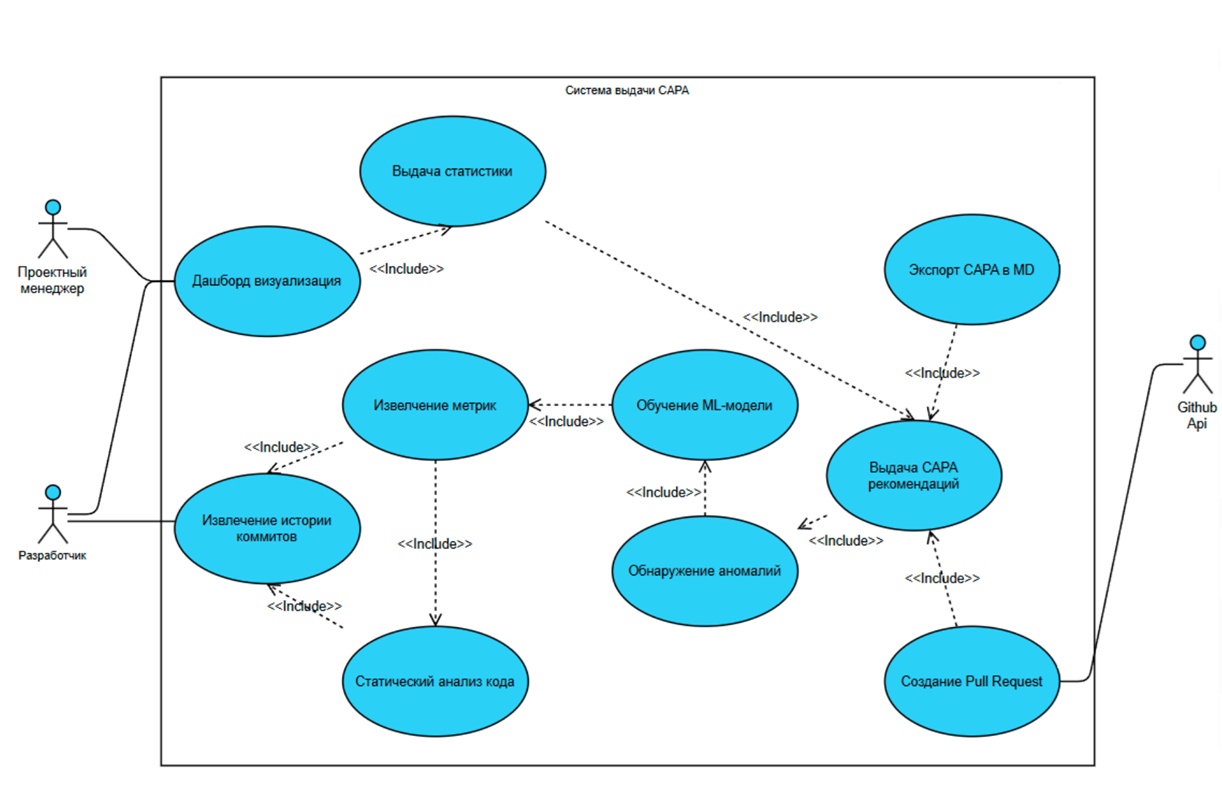
\includegraphics[width=0.9\textwidth]{my_folder/images/useCase (1).png}
	\caption{Use Case-диаграмма системы автоматического формирования CAPA}
	\label{fig:usecase}
\end{figure}


\section{Выводы} \label{ch1:conclusion}

Современные практики формирования CAPA на основе анализа репозиториев кода объединяют строгие процедуры управления качеством и динамическую ML-аналитику истории изменений. Классический цикл CAPA — сбор инцидентов, диагностика, планирование и проверка эффективности мер — дополняется JIT-предсказанием дефектов и классификацией коммитов на основе моделей машинного обучения, а также «бот-аналитикой» (TOM, GitHub Apps), когда система сама собирает метрики и создаёт pull-request’ы с рекомендациями. При выборе решения критичны автоматизируемость, интеграция в CI/CD, учёт истории коммитов и интерпретируемость результатов. Статические анализаторы (SonarQube) надёжно автоматизируются, но не отслеживают эволюцию проекта, а ML-модели улавливают сложные паттерны в истории, но требуют обучения и часто выступают «чёрным ящиком». Наименее работоспособным оказывается чистый QMS-софт без аналитики кода. Лучшие практики — это гибридный подход: статический анализ, ML-классификация и интеграция с баг-трекером для автосоздания задач CAPA.


	         	 % Глава 1
\ContinueChapterBegin % размещать главы <<подряд>> 
\chapter{Разработка метода, алгоритма, модели исследования} \label{ch2}

\section{Постановка задачи} \label{ch2:method_selection}

Для построения системы автоматического анализа коммитов GitHub каждое изменение представлено в виде вектора числовых признаков. Формально определим вектор признаков коммита как:
\begin{equation}
	c_i = \{a_i, d_i, t_i, f_i, \tau_i\, \gamma_i\},
\end{equation}

где:
\begin{itemize}
	\item \( a_i \) --- количество добавленных строк кода,
	\item \( d_i \) --- количество удаленных строк кода,
	\item \( t_i \) --- общее число изменений (сумма добавленных и удаленных строк),
	\item \( f_i \) --- количество измененных файлов,
	\item \( \tau_i \) --- время с момента последнего коммита.
	\item \( \gamma_i \) --- оценочная сложность изменений (суммарная цикломатическая сложность изменённых файлов).
\end{itemize}

Выбранное представление компактно описывает основные характеристики коммита и пригодно для обработки методами машинного обучения. Такие метрики широко используются в исследованиях по предсказанию дефектов коммитов: например, установлено, что с увеличением числа добавленных строк (\( a_i \)) растёт вероятность дефектного изменения.

Признак \( \gamma_i \) дополнительно учитывает сложность правок; например, при прочих равных более «тяжёлые» изменения могут требовать повышенного внимания. Таким образом, вектор \( c_i \) обеспечивает информативное и сжатое описание каждого коммита, пригодное для последующей автоматической обработки.

\section{Кластерный анализ коммитов} \label{ch2:problem_formulation}

Представленные вектора \( c_i \) рассматриваются как точки в \( R^5 \). Для первичной разметки коммитов на «нормальные» и «аномальные» применён метод кластеризации k-средних. Алгоритм k-means разбивает множество наблюдений на k кластеров, приписывая каждую точку кластеру с ближайшим центройдом. Выбирая небольшое число кластеров (например, k = 2), мы автоматически выявляем естественные группы коммитов по схожести признаков. Коммит считается потенциально аномальным, если он попадает в кластер с необычным центроидом или малой плотностью: например, кластер, содержащий коммиты с экстремально большим числом добавленных/удалённых строк или затронутыми файлами, трактуется как «аномальный».

Использование кластеризации вместо ручной установки порогов обладает рядом преимуществ:
\begin{itemize}
	\item Адаптивность. Границы между нормальными и аномальными коммитами определяются по распределению реальных данных, а не зависят от заранее заданных эвристик.
	\item Объективность. Модель сама выявляет естественные группы, устраняя субъективность эксперта при выборе порогов.
	\item Масштабируемость. Алгоритм эффективно обрабатывает большие массивы данных и может быть переиспользован без ручной перенастройки порогов.
\end{itemize}

Таким образом, кластеризация позволяет автоматически настроить «пороги аномальности» на конкретный набор коммитов, что делает обнаружение аномалий более адаптивным и надежным по сравнению с простыми эвристическими критериями.

\section{Классификация коммитов методом глубокого леса} \label{ch2:algorithm_selection}

После разметки коммитов на нормальные и аномальные на соответствующих метках обучается классификатор. В качестве модели используется глубокий лес (CascadeForestClassifier), основанный на идеях алгоритма gcForest. Это ансамблевый алгоритм, реализующий каскадную структуру из случайных лесов. На каждом уровне каскада обучаются несколько лесов решений; выходы лесов предыдущего уровня дополняют признаки для следующего уровня. Такая многоуровневая архитектура позволяет глубоко изучать представления данных без рекуррентный нейронный сетей.

Классификатор CascadeForestClassifier обучается на размеченных данных {\( c_i \), \( y_i \)} - где \( y_i \) - метка класса «нормальный/аномальный». После обучения модель выдаёт для нового коммита оценку вероятности его принадлежности к аномальному классу, то есть риска изменения. Численность уровней каскада может определяться автоматически (по критерию прироста качества), что позволяет глубокой модели хорошо работать при небольшом объёме обучающих данных, кроме того, глубокий лес имеет сравнительно мало гиперпараметров и демонстрирует высокую стабильность результатов.

Использование глубокого леса на размеченных данных даёт возможность уточнить исходную разметку кластеризацией: модель учитывает все признаки в совокупности и вырабатывает более точные границы между нормальными и аномальными коммитами. В результате этой стадии получается классификатор, который для каждого нового коммита вычисляет риск его аномальности.


\section{Заключение} \label{ch2:conclusion}

В этой главе сформулирована задача представления коммита в виде числового вектора признаков и описана двухэтапная схема автоматической классификации. Сначала при помощи алгоритма k-means выполняется первичное разбиение коммитов на «нормальные» и «аномальные» на основе их статистических характеристик. Затем на полученных метках обучается модель глубокого леса, уточняющая классификацию и прогнозирующая риск новых коммитов. Полученные оценки аномальности коммитов образуют основу для последующей генерации корректирующих действий (CAPA).
	         	 % Глава 2
\chapter{Разработка программного обеспечения} \label{ch3}

\section{Проектирование архитектуры системы} \label{ch3:sec1}

Архитектура включает компоненты для сбора и хранения данных, их интеллектуального анализа, а также представления результатов и выработки корректирующих и предупреждающих действий (CAPA). На диаграмме (рис. 3.1) прямоугольниками обозначены основные модули системы, а стрелками – потоки данных и событий между ними. Сплошные стрелки отображают основной поток обработки данных от источника (репозитория) до получения результатов анализа, тогда как пунктирные стрелки показывают обмен информацией с интерактивной панелью мониторинга и инициирование действий CAPA.

\begin{figure}[ht!]
	\centering
	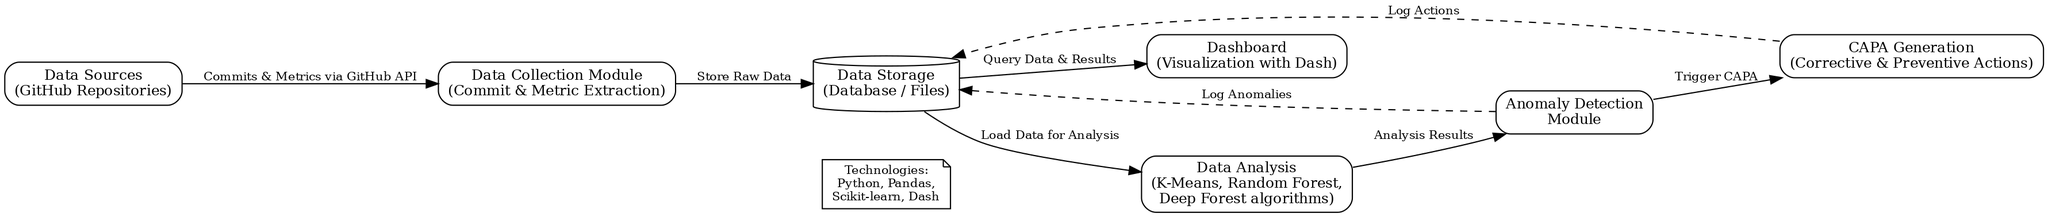
\includegraphics[width=1\textwidth]{my_folder/images/architect.png}
	\caption{Архитектура системы автоматического анализа коммитов GitHub}
	\label{fig:architecture}
\end{figure}

Основные компоненты архитектуры системы следующие:

\begin{itemize}
	\item Модуль сбора данных - отвечает за подключение к источникам данных (репозиториям GitHub) и извлечение информации о коммитах через API. Этот модуль собирает необходимые сырые данные: метаданные коммита (автор, метка времени, сообщение) и статистику изменений (количество добавленных/удалённых строк, изменённые файлы и пр.).
	\item Хранилище данных – обеспечивает сохранение полученных данных о коммитах для дальнейшей обработки. В качестве хранилища может использоваться реляционная база данных или файлы (например, CSV) в зависимости от объёма данных. Хранилище служит единой точкой, откуда аналитические модули загружают данные, а панель мониторинга получает актуальную информацию для визуализации.
	\item Модуль анализа данных – реализует обработку и анализ собранных данных с использованием методов машинного обучения. На этом этапе рассчитываются метрики коммитов (размеры изменений, сложность и др.), выполняется кластеризация (например, алгоритм k-средних) для выявления групп схожих изменений и применяется модель классификации (случайный лес, глубокий лес и др.) для определения рискованных коммитов. Результаты анализа (например, присвоенные каждому коммиту оценки риска или принадлежность к кластеру) передаются в модуль обнаружения аномалий и далее – на панель визуализации.
	\item Модуль обнаружения аномалий – специализируется на выявлении отклонений в шаблонах коммитов, в частности на аномальных временных интервалах между последовательными коммитами или нетипично крупными изменениями. Опираясь на результаты предыдущего этапа (рассчитанные метрики и кластеризацию) данный модуль идентифицирует события, выходящие за пределы нормального диапазона. Обнаруженные аномалии (например, чрезвычайно долгий промежуток между коммитами или всплеск исправлений ошибок) регистрируются и могут служить триггером для запуска процесса CAPA.
	\item Модуль генерации CAPA – формирует корректирующие и предупреждающие действия на основе выявленных проблемных ситуаций. Получая информацию о выявленной аномалии или рискованном коммите, модуль генерирует текстовые рекомендации (CAPA), направленные на исправление текущих проблем (корректирующие меры) и предотвращение подобных ситуаций в будущем (превентивные меры). Эти рекомендации могут затем автоматически фиксироваться в системе (например, добавляться в журнал действий или отправляться в виде уведомлений команде разработки).
	\item Панель визуализации (Dashboard) – интерактивное веб-приложение, реализованное с использованием фреймворка Dash, предназначено для отображения результатов анализа. Дашборд запрашивает из хранилища необходимые данные и визуализирует их в виде графиков и метрик. Он также отображает обнаруженные системой аномалии и сгенерированные рекомендации CAPA, позволяя пользователям оперативно получать информацию о состоянии проекта. Через панель разработчики могут просмотреть ключевые показатели (например, частоту коммитов, размер изменений), выявленные риски и предложенные действия по их устранению.
\end{itemize}

Предложенная архитектура обеспечивает модульность и расширяемость системы. Каждый компонент выполняет свою чётко определённую роль и взаимодействует с другими через ограниченные интерфейсы (например, совместный доступ к хранилищу или передачу сигналов об аномалиях). Такое разделение обязанностей упрощает отладку и поддержку системы, позволяя независимо совершенствовать сбор данных, аналитические алгоритмы или визуализацию. В результате спроектированная архитектура создаёт основу для эффективной реализации системы автоматического анализа коммитов и формирования CAPA.

\section{Извлечение и обработка данных из GitHub} \label{ch3:sec2}

На этапе сбора данных реализован класс GitHubRepoAnalyzer, инкапсулирующий функциональность подключения к API GitHub и анализа истории коммитов целевого репозитория. Данный класс обеспечивает получение списка коммитов, извлечение деталей каждого коммита и расчёт необходимых метрик для последующего анализа. Ниже перечислены ключевые методы и процедуры, реализованные в GitHubRepoAnalyzer:
\begin{itemize}
	\item \textbf{Аутентификация и подключение к репозиторию}. В конструкторе класса выполняется аутентификация к GitHub через токен доступа и инициализируется подключение (С помощью запросов REST API). Это позволяет в дальнейшем безопасно вызывать методы GitHub API для чтения данных.
	\item \textbf{Получение списка коммитов}. Метод \verb|fetch_commits(repo_name)| отправляет запрос к GitHub API для получения списка коммитов указанного репозитория \verb|repo_name|. Он возвращает итератор или список объектов коммитов (содержащих информацию о каждом коммите: SHA-хеш, автор, дата, сообщение, статистика изменений и др.). При необходимости данный метод может поддерживать постраничную загрузку, чтобы обработать весь исторический ряд коммитов для крупных проектов.
	\item \textbf{Извлечение данных коммита и расчёт метрик}. Для каждого коммита выполняется обработка деталей. Метод \verb|analyze_commit(commit)| рассчитывает такие показатели как: количество изменений в коде: число добавленных строк кода (additions), удалённых строк (deletions) и общее изменение (\verb|total_changes|, сумма добавленных и удалённых строк) на основе статистики диффа, предоставляемой GitHub. Затронутые файлы: число файлов, изменённых в данном коммите. Этот показатель косвенно отражает масштабы влияния изменения на кодовую базу (коммит, затрагивающий много файлов, вероятно, более комплексный). Интервал времени с предыдущего коммита: разность во времени (в днях) между текущим коммитом и предыдущим по времени. Первый коммит в истории не имеет предыдущего, для него интервал определяется как 0. Данный показатель позволяет отслеживать ритм работы над проектом. Наличие признаков багфикса: анализ текста сообщения коммита на наличие ключевых слов, указывающих на исправление ошибки (например, "fix", "bug", "error"). Если такие слова присутствуют, для коммита устанавливается флаг, что он относится к исправлению дефекта. Это служит бинарным признаком (0/1), указывающим на потенциально проблемный характер изменения (коммит, содержащий багфикс, свидетельствует о том, что ранее в коде была проблема). Оценка сложности изменения: введена дополнительная метрика сложности, оценивающая масштаб и потенциальную сложность внесённого изменения. В рамках данной работы сложность коммита приближённо характеризуется совокупностью других метрик – например, общим числом изменённых строк кода и количеством затронутых файлов. Предполагается, что коммиты с большим числом изменений и широким охватом файлов более сложны для понимания и проверки.
	\item \textbf{Сохранение и предварительная обработка}. Собранные по каждому коммиту данные сохраняются либо в оперативной памяти (в виде структуры pandas.DataFrame), либо сразу в файловое хранилище. В текущей реализации происходит запись метрик коммитов в CSV-файл (\verb|repository_data.csv|) с колонками: репозиторий, SHA коммита, автор, дата и время, сообщение, добавления, удаления, всего изменений, файлов изменено, интервал с предыдущим коммитом, признак багфикса и поле под флаг CAPA. Этот датасет затем используется на следующих этапах анализа. Перед моделированием данные могут дополнительно очищаться: устраняются дубликаты, проверяется корректность временных меток, при необходимости вычисляются дополнительные поля (например, средняя частота коммитов для автора или кумулятивные метрики).
\end{itemize}

В результате работы GitHubRepoAnalyzer формируется структурированный набор данных обо всех коммитах репозитория со значимыми характеристиками каждого изменения. Такой подход автоматизирует извлечение данных, избавляя от ручного сбора статистики, и гарантирует единообразие вычисленных метрик. Полученные данные служат основой для применения алгоритмов машинного обучения на следующем этапе. Таким образом, реализация модуля сбора и предварительного анализа данных обеспечивает подготовку качественного обучающего множества для последующего моделирования CAPA.


\section{Интеграция модели глубокого леса} \label{ch3:sec3}

Для выявления потенциально проблемных коммитов в системе используется модель классификации на основе алгоритма глубокого леса (Deep Forest). Прежде чем обучить модель, необходимо сформировать обучающую выборку, включающую признаки коммитов и целевой признак (метку), указывающую, требуется ли для данного коммита выработка CAPA. В текущей реализации разметка данных выполнена на основе эвристических правил и результатов предварительного анализа:
Коммит помечается как «требующий CAPA» (метка 1), если он удовлетворяет одному или нескольким критериям риска: например, содержит исправление ошибки (выявлено по ключевым словам в сообщении), имеет чрезвычайно большой объём изменений (значительно превышающий типичные значения по проекту) или связан с аномально долгим интервалом отсутствия активности перед ним. Такие коммиты свидетельствуют о возникновении проблем (дефект в коде, накопление большого пакета изменений, сбой в регулярности разработки), что требует принятия мер.
Коммиты, не соответствующие этим условиям, считаются обычными (метка 0). Они характеризуются типичным размером и содержанием изменений, не содержат явных признаков багфиксов и происходят с регулярной частотой, соответствующей нормальному ходу разработки.

На основе класса GitHubRepoAnalyzer из предыдущего раздела формируются признаки для модели. В качестве входных признаков (features) для каждого коммита используются:
\begin{enumerate}
	\item Общее количество изменённых строк кода (\verb|total_changes|), отражающее размер коммита.
	\item Число затронутых файлов (\verb|files_changed|).
	\item Интервал времени с предыдущего коммита (\verb|time_since_last_commit|).
	\item Наличие багфикса (булев флаг \verb|bug_fix_flag|, 1 – если в сообщении коммита обнаружены слова, указывающие на исправление ошибки).
	\item Производные или комплексные признаки сложности (например, комбинация из первых двух: большие \verb|total_changes| при большом \verb|files_changed| могут усиливать оценку сложности).
\end{enumerate}


Перед обучением количественные признаки масштабируются к сопоставимому диапазону. Если данных для обучения относительно немного, может применяться кросс-валидация или бутстреп-перемешивание для более устойчивого обучения модели. Модель глубокого леса, используемая в системе, реализована в виде классификатора CascadeForestClassifier. Данный алгоритм представляет собой каскадную композицию ансамблей решающих деревьев, альтернативный подход глубокого обучения для табличных данных. Вместо одной стадии обучения случайного леса, CascadeForest выстраивает несколько уровней (layers) из ансамблей (случайных лесов и полностью случайных деревьев), последовательно обрабатывающих данные. На каждом уровне входные признаки дополняются выходами предыдущего уровня (например, вероятностями классов), что позволяет каскаду постепенно «усложнять» представление данных и улучшать качество классификации. Обучение продолжается до тех пор, пока добавление нового уровня улучшает качество на валидационном подмножестве, либо останавливается при достижении заданного числа уровней.

В ходе обучения CascadeForestClassifier на собранных данных коммитов каждый уровень каскада строит несколько случайных лесов. Так, на первом уровне может быть обучено два случайных леса: один на исходных признаках, другой на той же выборке, но с иной инициализацией. Результаты (предсказанные вероятности классов для каждого примера) затем прикрепляются к признакам, и второй уровень обучает новые леса с расширенным пространством признаков. Такой подход позволяет модели выявлять сложные нелинейные зависимости в данных коммитов, которые мог пропустить один «плоский» алгоритм.

После тренировки модели на обучающей выборке её качество проверяется на отложенных данных (тестовом наборе) либо с помощью кросс-валидации. Оценка показала, что модель глубокого леса успешно классифицирует коммиты с точки зрения необходимости CAPA, превосходя по некоторым метрикам более простой алгоритм случайного леса. Например, для множества тестовых коммитов были корректно выявлены все случаи известных проблемных изменений при небольшом количестве ложных срабатываний.

Анализ важности признаков показал, что наибольшее влияние на решение о рискованности коммита оказывают объём внесённых изменений кода и наличие багфикса. Так, признак общего количества изменённых строк получил наивысший вес (самый информативный), поскольку крупные коммиты чаще связывались с последующими проблемами. Следующими по важности идут временной интервал (длительные паузы перед коммитом могли указывать на накопление изменений или упущенные баги) и индикатор исправления ошибок. Число затронутых файлов сыграло заметную, но меньшую роль. Анализ значимости подтверждает, что выбранные метрики обоснованно влияют на решение модели и соответствуют интуитивным представлениям: действительно, чем больше и реже изменения, тем выше вероятность необходимости дополнительных действий.

Таким образом, посредством обучения модели CascadeForestClassifier была получена интеллектуальная подсистема, способная на основе метрик коммита предсказывать необходимость CAPA. Этот классификатор служит ядром системы, автоматически оценивая каждый новый коммит и выделяя наиболее рискованные, требующие внимания разработчиков или менеджеров проекта.

\section{Реализация панели визуализации на фреймворке Dash} \label{ch3:sec4}

Визуализационная панель разработана с использованием фреймворка Dash - инструмента создания адаптивных и интерактивных веб-приложений на Python.

Интерфейс приложения разбит на несколько вкладок. Например, есть обзорная вкладка с ключевыми метриками и графиками по всем коммитам, отдельная вкладка с детальной аналитикой (графики изменений по авторам, времени и т.п.) и вкладка «Рекомендации», где в табличном виде выводится список сформированных системой корректирующих действий (CAPA) для выявленных аномалий. Для построения визуализаций используются возможности библиотеки Plotly: гистограммы (распределение числа коммитов по дням недели, авторам, величине изменений), круговые диаграммы (распределение изменений по типам или модулям), тепловые карты активности коммитов во времени и пр. Такие графики позволяют исследовать данные «вживую» и лучше выявлять закономерности

\begin{itemize} 
	\item \textbf{Структура и вкладки:} Панель разбита на тематические разделы. Например, основная вкладка показывает общее состояние репозитория (гистограммы коммитов, круговые диаграммы распределения изменений по авторам и файлам), другая – показывает детальную статистику во временном разрезе, а вкладка «Рекомендации» содержит список автоматических советов (CAPA) по улучшению процесса разработки. 
	\item \textbf{Типы визуализаций:} Используются интерактивные графики Plotly – гистограммы, круговые (pie) диаграммы, тепловые карты и линейные графики. Все эти диаграммы являются кликабельными, что позволяет пользователю изучать подробные данные.
	\item \textbf{Интерактивность:} За динамическое поведение отвечает механизм callback-функций Dash. При выборе фильтров (например, диапазона дат, конкретного автора или папки проекта) соответствующие графики автоматически обновляются.
	\item \textbf{Адаптивность интерфейса:} При создании приложения использованы компоненты \verb |dash_bootstrap_components| и тема Bootstrap. В частности, при инициализации приложения подключена тема Bootstrap (\verb|external_stylesheets=[dbc.themes.BOOTSTRAP]|), что гарантирует адаптивное размещение элементов на экране. В итоге панель корректно отображается на различных устройствах и экранах, сохраняя удобство восприятия.
	
\end{itemize}

Всё это делает дашборд удобным инструментом мониторинга: наглядные диаграммы и список рекомендаций позволяют быстро оценить состояние репозитория и принять решения на основе анализа данных.

\section{Интеграция компонентов в единую систему} \label{ch3:sec5}

Модули сбора данных, анализа и визуализации объединены в единую конвейерную цепочку обработки. Dash-приложение напрямую подключается к Python-моделям и хранилищам данных, что позволяет строить «сквозную» аналитику. В частности, Dash умеет обращаться к базам данных и другим источникам через Python-коннекторы, выполняя запросы и продвинутый анализ «на лету». роме того, фреймворк Dash хорошо интегрируется с библиотеками обработки данных (Pandas, NumPy и др.), что облегчает построение комплексных аналитических приложений.

Работа системы организована следующим образом:
\begin{itemize} 
	\item \textbf{Сбор данных:} Модуль извлечения с помощью HTTP запросов обращается к GitHub, получает историю коммитов заданных репозиториев и сохраняет её в удобном формате. Собираются метрики коммита: SHA, автор, дата, количество добавленных/удалённых строк, список затронутых файлов и т.д. Этот этап можно запускать вручную при появлении новых данных.
	 \item \textbf{Обработка и анализ:} Загруженные данные проходят первичную обработку: вычисляются дополнительные признаки (интервалы между коммитами, суммарные изменения), после чего применяется кластеризация (KMeans) для определения нормальных границ изменений. Затем обучаются модели машинного обучения Глубокого Леса для классификации коммитов на нормальные и аномальные.
	 \item \textbf{Генерация рекомендаций (CAPA):} На основе классификации система формирует корректирующие и предупредительные действия для выявленных аномалий. Для каждого «подозрительного» коммита вычисляются рекомендации (например, обратить внимание на высокую частоту изменений или большой объём кода) и при необходимости автоматически создаётся pull request с этими рекомендациями.
	 \item \textbf{Визуализация результатов:} После анализа результаты поступают на дашборд. Dash-приложение загружает актуальный набор данных (или обращается к подготовленной статистике) и отображает их в виде графиков и таблицы рекомендаций. Таким образом, пользователь получает единый интерфейс, где и графики, и текстовые CAPA-сообщения согласованы между собой.
	 \item \textbf{Автоматическое обновление:} При появлении новых коммитов цикл повторяется: система периодически выполняет сбор свежих данных, прогон анализов и обновляет панель. Пользователи получают актуальную информацию без необходимости ручного запуска каждого этапа – весь процесс сквозной автоматизации обеспечивает своевременное отображение рекомендаций и метрик.
\end{itemize}

\section{Выводы} \label{ch3:sec6}

Разработанная система была реализована в соответствии с поставленными задачами: созданы отдельные модули для извлечения данных коммитов, их анализа и визуализации. Модульный подход позволяет четко разделять функциональность и поддерживать каждый компонент независимо. 

Достигнуты ключевые цели проекта: архитектура системы является модульной и легко расширяемой – новые алгоритмы анализа или метрики могут быть добавлены без переделки остального кода. Процесс анализа коммитов полностью автоматизирован: от сбора данных до отображения результатов на панели не требуется ручного участия, что облегчает регулярный мониторинг качества разработки.  В ходе работы создан интерактивный дашборд на Dash, обеспечивающий гибкую визуализацию и удобный интерфейс для разработчиков. Это позволяет в реальном времени отслеживать состояние репозитория и эффективно использовать полученные рекомендации для улучшения кода.

Перспективы развития проекта включают расширение функционала: можно добавить новые метрики коммитов и шаблоны анализа, интегрировать систему с инструментами CI/CD и сервисами контроля качества кода, а также исследовать применение нейросетевых моделей для повышения точности предсказаний CAPA.           	 % Глава 3
\chapter{Тестирование системы формирования CAPAs на основе изменений репозитория кода} \section{Введение}
В ходе тестирования проверяется работоспособность разработанного инструментария и выполняются поставленные в работе задачи. Основными целями данного этапа являются:
\begin{itemize}
	\item Проверка корректности функционирования пользовательского интерфейса и всех компонентов системы (сбора данных, анализа репозиториев, генерации рекомендаций).
	\item Оценка качества работы классификатора рисковых коммитов на реальных данных, полученных из активных репозиториев.
	\item Тестирование модели генерации CAPA (рекомендаций исправлений) для выявления ошибок и неточностей в алгоритме.
	\item Модульное и нагрузочное тестирование компонентов системы для выявления багов на уровне отдельных модулей и проверки масштабируемости на больших репозиториях.
\end{itemize}
Таким образом, экспериментальное тестирование охватывает проверку как функциональных характеристик (работа интерфейса, правильность алгоритмов), так и нефункциональных (надёжность, производительность) аспектов системы.

\section{Методика проведения тестирования}
Для проверки системы было выбрано несколько тестовых репозиториев с собственными разработками: \texttt{Tq}, \texttt{scherBook}, \texttt{NTO2024-2025}, а также репозитории предоставленные сторонними разработчиками и студентами, которые согласились поучаствовать в тестировании и апробации проекта: \texttt{urlagushka/polytech-labs}, \texttt{urlagushka/h8-pipeline}, \texttt{AlPakh/topotik-backend}, \texttt{AlPakh/topotik-frontend}, \texttt{Pacan4ik/tf-idf}, \texttt{Pacan4ik/tinkoff-course-spring2023}. Эти проекты содержат достаточно разнообразный код (на Java, Python, JavaScript, C++) и различную историю изменений, что обеспечивает репрезентативность данных.

\begin{longtable}{|p{3.5cm}|p{2.2cm}|p{2cm}|p{3cm}|p{4.5cm}|}
	\caption{Описание репозиториев, использованных в тестировании}
	\label{tab:test_repos} \\
	\hline
	\textbf{Репозиторий} & \textbf{Язык(и)} & \textbf{Кол-во коммитов} & \textbf{Тип проекта} & \textbf{Краткое описание} \\
	\hline
	\endfirsthead
	
	\multicolumn{5}{c}{{\tablename\ \thetable{}}} \\
	\hline
	\textbf{Репозиторий} & \textbf{Язык(и)} & \textbf{Кол-во коммитов} & \textbf{Тип проекта} & \textbf{Краткое описание} \\
	\hline
	\endhead
	
	\hline \multicolumn{5}{r}{{}} \\
	\endfoot
	
	\hline
	\endlastfoot
	
	\texttt{jup-ag/
		pyth-
		crosschain} & Python, Solidity & 3692 & Инфраструк-
		тура Web3 & Форк проекта Jup-ag с доработками Pyth network: кроссчейн модуль для верификации транзакций. \\
	\hline
	\texttt{Pacan4ik/
		tinkoff-course-
		spring2023} & Java & 188 & Курсовой проект & Проект на Java Spring Boot с интеграцией Telegram-бота и веб-интерфейсом. \\
	\hline
	\texttt{urlagushka/
		h8-pipeline} & Python & 110 & ML/AI пайплайн & Инициализатор проекта на базе Hailo SDK; используется для компьютерного зрения. \\
	\hline
	\texttt{AlPakh/
		topotik-
		backend} & Python (FastAPI) & 38 & Серверная часть & REST API бэкенд с авторизацией, ORM-моделями и обработкой карт. \\
	\hline
	\texttt{AlPakh/
		topotik-
		frontend} & JavaScript (Vue) & 27 & Клиентская часть & Vue-приложение с маршрутизацией, формами и подключением к API. \\
	\hline
	\texttt{Pacan4ik/
		tf-idf} & Python & 36 & Алгоритм обработки текста & Базовая реализация TF-IDF для анализа текстов на русском языке. \\
	\hline
	\texttt{Ausland3r/
		NTO2024-2025} & Python & 69 & Учебный проект & Материалы к проекту "Умный город" для школьников; используется в рамках NTO. \\
	\hline
	\texttt{urlagushka/
		polytech-labs} & C++, Java & 82 & Учебный проект & Набор лабораторных работ по программной инженерии; содержит решения на нескольких языках. \\
	\hline
	\texttt{Ausland3r/
		scherBook} & JavaScript & 39 & Веб-приложение & Клиентское приложение для платформы книгообмена; реализован основной UI. \\
	\hline
	\texttt{Ausland3r/
		Tq} & Python & 40 & Фреймворк для тестов & Небольшой собственный фреймворк на базе Pytest и Pydantic. \\
\end{longtable}

\section{Сравнение моделей классификации}

Для оценки эффективности алгоритмов машинного обучения в задаче предсказания рисковых коммитов был разработан универсальный класс \texttt{CommitRiskModel}. Он предоставляет единый интерфейс к различным классификаторам из \texttt{scikit-learn}, а также \texttt{deep-forest}. Класс реализует методы \texttt{fit()}, \texttt{predict()}, \texttt{predict\_proba()}, \texttt{feature\_importances()} и \texttt{evaluate\_model()}.

Для сравнения были обучены и протестированы десять моделей на выборках коммитов с автоматически определёнными метками риска. Эксперименты проводились как на небольших проектах (в пределах сотни коммитов), так и на объёмном репозитории \texttt{jup-ag/pyth-crosschain} (более 3000 коммитов).

\begin{table}[h!]
	\centering
	\caption{Сравнение моделей классификации на малом проекте (Pacan4ik/tinkoff-course-spring2023)}
	\label{tab:metrics_comparison_small_extended}
	\resizebox{\textwidth}{!}{
		\begin{tabular}{|l|c c c c|}
			\hline
			\textbf{Модель} & \textbf{Precision} & \textbf{Recall} & \textbf{F1-score} & \textbf{ROC-AUC} \\
			\hline
			LogisticRegression & 0.600 & 1.000 & 0.750 & 0.990 \\
			RandomForest       & 0.800 & 0.667 & 0.727 & 0.979 \\
			ExtraTrees         & 0.800 & 0.667 & 0.727 & 0.984 \\
			GradientBoosting   & 1.000 & 0.833 & 0.909 & 0.995 \\
			AdaBoost           & 1.000 & 0.833 & 0.909 & 0.979 \\
			XGBoost            & 0.800 & 0.667 & 0.727 & 0.979 \\
			LightGBM           & 0.800 & 0.667 & 0.727 & 0.958 \\
			CatBoost           & 0.833 & 0.833 & 0.833 & 0.990 \\
			SVM                & 0.833 & 0.833 & 0.833 & 0.990 \\
			DeepForest         & 0.833 & 0.833 & 0.833 & 0.990 \\
			\hline
		\end{tabular}
	}
\end{table}

На проекте Pacan4ik/tinkoff-course-spring2023 лучшие результаты по полноте (Recall = 0.833) и F1-score (0.909) показывают модели GradientBoosting и AdaBoost. Модели DeepForest, SVM и CatBoost демонстрируют сбалансированное сочетание метрик с F1 около 0.833 и высоким ROC-AUC (0.990), что свидетельствует о стабильной и надёжной работе. LogisticRegression достигает максимальной полноты (Recall = 1.0), но при этом точность ниже (Precision = 0.6), что говорит о склонности к избыточному помечанию коммитов как рисковых с увеличением числа ложных срабатываний. Модели RandomForest, ExtraTrees и XGBoost показывают одинаковые метрики, отражающие умеренный баланс между точностью и полнотой. В целом, DeepForest проявляет хорошую устойчивость при обучении на небольшом объёме данных.

\begin{table}[h!]
	\centering
	\caption{Сравнение моделей классификации на большом проекте}
	\label{tab:metrics_comparison_large_extended}
	\resizebox{\textwidth}{!}{
		\begin{tabular}{|l|c c c c|}
			\hline
			\textbf{Модель} & \textbf{Precision} & \textbf{Recall} & \textbf{F1-score} & \textbf{ROC-AUC} \\
			\hline
			LogisticRegression & 0.696 & 0.941 & 0.800 & 0.996 \\
			RandomForest       & 0.917 & 0.647 & 0.759 & 0.995 \\
			ExtraTrees         & 0.933 & 0.824 & 0.875 & 0.998 \\
			GradientBoosting   & 0.933 & 0.824 & 0.875 & 0.933 \\
			AdaBoost           & 0.875 & 0.824 & 0.848 & 0.952 \\
			XGBoost            & 0.867 & 0.765 & 0.812 & 0.962 \\
			LightGBM           & 0.818 & 0.529 & 0.643 & 0.946 \\
			CatBoost           & 0.867 & 0.765 & 0.812 & 0.994 \\
			SVM                & 0.938 & 0.882 & 0.909 & 0.999 \\
			DeepForest         & 0.842 & 0.941 & 0.889 & 0.996 \\
			\hline
		\end{tabular}
	}
\end{table}

На большом проекте \texttt{pyth-crosschain} наблюдается более разнообразная картина качества моделей. Модель SVM показывает наилучшие результаты по ключевым метрикам: высокая точность (0.938), хорошая полнота (0.882), сбалансированный F1-score (0.909) и практически идеальный ROC-AUC (0.999). Это говорит о том, что SVM эффективно выявляет рисковые коммиты, минимизируя как ложные срабатывания, так и пропуски.
Ансамблевые модели ExtraTrees и GradientBoosting также демонстрируют высокую полноту (Recall = 0.824) и хорошие показатели по остальным метрикам, показывая стабильность и надёжность на больших данных.
LogisticRegression и DeepForest выделяются очень высокой полнотой (около 0.94), что означает, что они почти не пропускают рисковые коммиты. Однако у DeepForest точность немного ниже, вероятно из-за особенности архитектуры каскадных слоёв, которая может быть чувствительна к шуму в данных, что приводит к большему количеству ложных срабатываний.
В целом, SVM показывает наилучшее сочетание точности и полноты, что делает эту модель предпочтительным выбором для задач классификации рисковых коммитов в больших репозиториях.

Таким образом, можно выделить следующие рекомендации:
\begin{itemize}
	\item Для небольших проектов с ограниченной историей коммитов предпочтительнее использовать \texttt{DeepForest} и ансамблевые методы, чтобы минимизировать пропущенные риски и достичь сбалансированных метрик.
	\item Для крупных репозиториев рекомендуется \texttt{SVM} и методы градиентного бустинга \texttt{XGBoost} \texttt{CatBoost} как наиболее устойчивые и точные модели.
\end{itemize}

В итоге можно с уверенностью сказать, что разработанный унифицированный класс \texttt{CommitRiskModel} позволяет гибко подключать и тестировать разные алгоритмы без необходимости переписывать код, что делает систему легко масштабируемой и адаптируемой под различные сценарии и объёмы данных.

\section{Модульное тестирование}

Для обеспечения качества и надёжности разработанного программного обеспечения выполнено модульное тестирование ключевых компонентов системы. В рамках тестирования было создано и выполнено 12 отдельных тестов, охватывающих основные сценарии работы и критичные граничные случаи. Основные направления тестирования и проверяемые аспекты включают:

\begin{itemize}
	\item \texttt{ml\_model.py}:
Проверялись основные методы обучения и предсказания моделей машинного обучения. Тесты, такие как \verb|test_model_extremes_and_balanced_cases| и \verb|test_model_predict_|
\verb|proba_output|, гарантировали корректную работу метода \texttt{fit()}, проверяли способность модели обучаться на реальных и частично неполных данных, а также корректно обрабатывать ситуации с отсутствием или неполнотой входных данных. Валидация предсказаний включала проверку возвращаемых значений — скалярных вероятностей в диапазоне от 0 до 1.

Данный набор тестов помогает своевременно обнаруживать ошибки, связанные с изменениями в логике обучения и предсказания, предотвращая ошибки при работе с моделями машинного обучения.

\item \texttt{repository\_analysis.py}:

Проверялся процесс сбора и обработки статистики по коммитам из репозитория. В тестах, например, \texttt{test\_repository\_empty\_and\_corrupted} были учтены разные ситуации: работа с нормальным репозиторием с несколькими коммитами, а также с пустым репозиторием или с некорректными данными или отсутствующими файлами. Тесты гарантировали, что модуль не выдаёт ошибок при отсутствии данных, а возвращает корректные пустые структуры.  

Это снижает риск сбоев в работе системы при взаимодействии с нестандартными или пустыми репозиториями.

\item \texttt{recommendations.py}: 

Проверялись функции генерации рекомендаций на основе анализа изменений в коммитах. Тест \texttt{test\_recommendations\_extreme\_commit} моделирует ситуации с коммитами без добавленных строк кода, наличием уже существующих рекомендаций. Проверялась корректность формируемых списков рекомендаций.

Это позволяет гарантировать, что рекомендации будут релевантными и не содержат дублирующей или ошибочной информации.

\item \texttt{app.py}:

Этот модуль содержит ключевые функции, обеспечивающие загрузку и анализ данных из репозиториев, обучение модели машинного обучения и обновление табличного представления результатов. Тесты \texttt{test\_load\_and\_analyze\_repos}, \texttt{test\_train\_and\_update\_model} и \texttt{test\_update\_tabs} проверяют корректность выполнения основных операций.
\end{itemize}

Все тесты были автоматизированы с использованием фреймворка \texttt{pytest} и обеспечили покрытие ключевых функциональных частей системы более чем на \verb|75%|. Такой уровень тестового покрытия подтверждает надёжность и стабильность реализации, а также значительно упрощает сопровождение и дальнейшее развитие кода, обеспечивая своевременное выявление регрессий и ошибок.

\begin{center}
	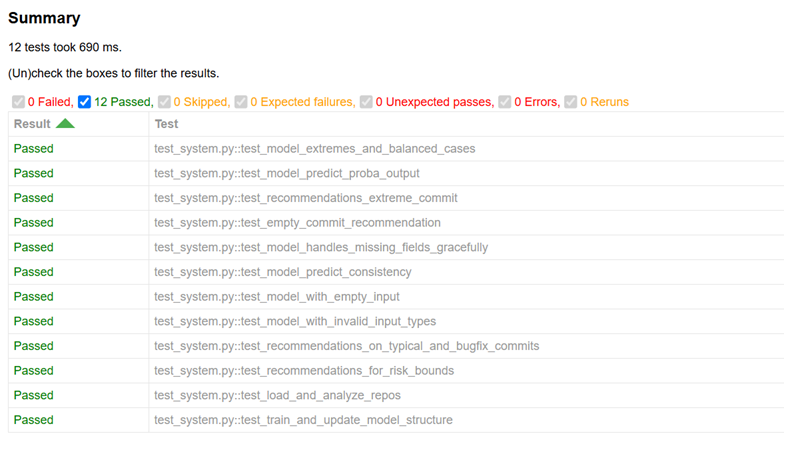
\includegraphics[width=\textwidth]{my_folder/images/test_result.png}
	\captionof{figure}{Отчёт с результатом прогона автотестов в pytest-html}
	\label{fig:test_pytest}
\end{center}

\begin{figure}[H]
	\centering
	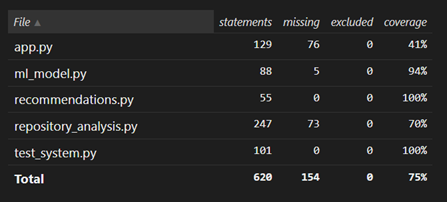
\includegraphics[width=0.8\textwidth]{my_folder/images/coverage.png}
	\caption{Отчёт по покрытию автотестами в pytest-cov}
	\label{tab:test_pytest2}
\end{figure}


\section{Мутационное тестирование}

В дополнение к обычным unit- и интеграционным тестам был подготовлен отдельный набор мутационных тестов.
Основная задача ­— проверить, насколько надёжно текущая реализация
\texttt{CommitRiskModel} и генератор рекомендаций защищены от ошибок
валидации, пограничных сценариев и тривиальных изменений логики.

\vspace{0.7em}
\subsection{Итоги прогона}

\begin{itemize}
	\item Сгенерировано~16 мутантов для~файла \texttt{ml\_model.py}.
	\item Выбито (\textit{DETECTED})~5, выжило (\textit{SURVIVED})~11.  
	Актуальный mutation-score: $\frac{5}{16}\!\times\!100 \approx 31\,\%$.
\end{itemize}

Порог в~80--90\,\% обычно считается «хорошим»,
поэтому результат в~31\,\% наглядно показывает,
что тест-покрытие пока ловит лишь треть потенциальных проблем.
Тем не менее, даже при таком проценте удалось найти и исправить ряд проблем.

\vspace{0.7em}
\subsection{Что удалось обнаружить мутационным тестированием}

\begin{enumerate}
	\item Пропущенные обязательные поля.
	Первые запуски выявили, что модель молча принимала коммиты без
	\verb|avg_file_history| или \verb|message_length|.  
	Добавлена строгая валидация (\verb|_validate_commits|),
	теперь отсутствие поля вызывает \verb|KeyError|.
	
	\item Отрицательные и строковые значения.
	Мутанты, подставляющие \verb|-5| вместо числа добавленных строк
	или строку ``ten'', приводили к некорректным вычислениям.
	Дополнительные проверки типов и границ теперь
	выбрасывают \verb|ValueError| до момента обучения.
	
	\item Некачественные рекомендации.
	Мутации в части генератора рекомендаций показали,
	что при высоком риске не всегда выводилась фраза
	«углублённое код-ревью». Тесты стали проверять
	не жёсткую строку, а наличие ключевого слова,
	что снизило ложные отрицания.
	
	\item Неверные вероятности \texttt{predict\_proba()}.
	Подмена метода на версию, возвращающую значения $>1$,
	выявила отсутствие проверок диапазона.  
	В ответ была добавлена assert-проверка и дополнительные
	юнит-тесты на корректность нормировки.
\end{enumerate}

Для дальнейшего повышения показателя планируется:

\begin{itemize}
	\item добавить тесты, проверяющие влияние
	\verb|author_name=None| и крайние значения \verb|message_length|;
	\item игнорировать эквивалентные мутанты при помощи директивы
	\texttt{\# pragma: no mutate}, чтобы не искажать итоговый процент.
\end{itemize}

Таким образом, даже при неброском mutation-score
мутационные тесты уже помогли выявить критичные узкие места
и сформировали список точек для доработки.
	

\section{Нагрузочное тестирование}

Нагрузочное тестирование проводилось с целью оценки производительности системы при работе с крупными репозиториями. В качестве тестового примера был выбран репозиторий \texttt{jup-ag/pyth-crosschain} с более чем 3000 коммитов. Тестирование выполнялось на машине со следующими характеристиками: процессор AMD Ryzen 9 7900X, 16 ГБ оперативной памяти и SSD-накопитель.

\begin{itemize}
	\item Общее время обработки полного репозитория составило 46 минут. Основная часть времени затрачивается на последовательный запуск статического анализа (Pylint, Checkstyle) для сотен файлов. Дополнительное время уходит на загрузку коммитов через API GitHub, особенно при большом количестве коммитов в репозитории.
	
	\item Наиболее ресурсоёмкой подсистемой оказался статический анализ: последовательный запуск линтеров на большом количестве файлов существенно увеличивает нагрузку на ресурсы компьютера. Максимальная загрузка CPU достигала 53\%, а использование оперативной памяти — до 8 ГБ.
\end{itemize}
Для ускорения работы возможно применение кеширования результатов анализа и параллельной обработки файлов. Для избежания повторной загрузки данных с GitHub система сохраняет локальную копию репозитория. Поскольку API GitHub имеет ограничения по скорости и количеству запросов, локальный клон позволяет минимизировать обращения к API и работать с полной историей и файлами непосредственно на диске, что ускоряет повторный анализ уже загруженных репозиториев. Также чтобы не было необходимости постоянно запускать систему для получения рекомендаций весь список рекомендаций сохраняется локально в md файл и отправляется в отдельную ветку в удаленном репозитории.


В целом система стабильно справлялась с обработкой крупного репозитория, обеспечивая корректные результаты и бесперебойную работу. Максимальная нагрузка приходилась на этап анализа качества кода. Полученные результаты подтверждают, что разработанные компоненты способны эффективно работать с реальными проектами значительных размеров.

\begin{figure}[ht]
	\centering
	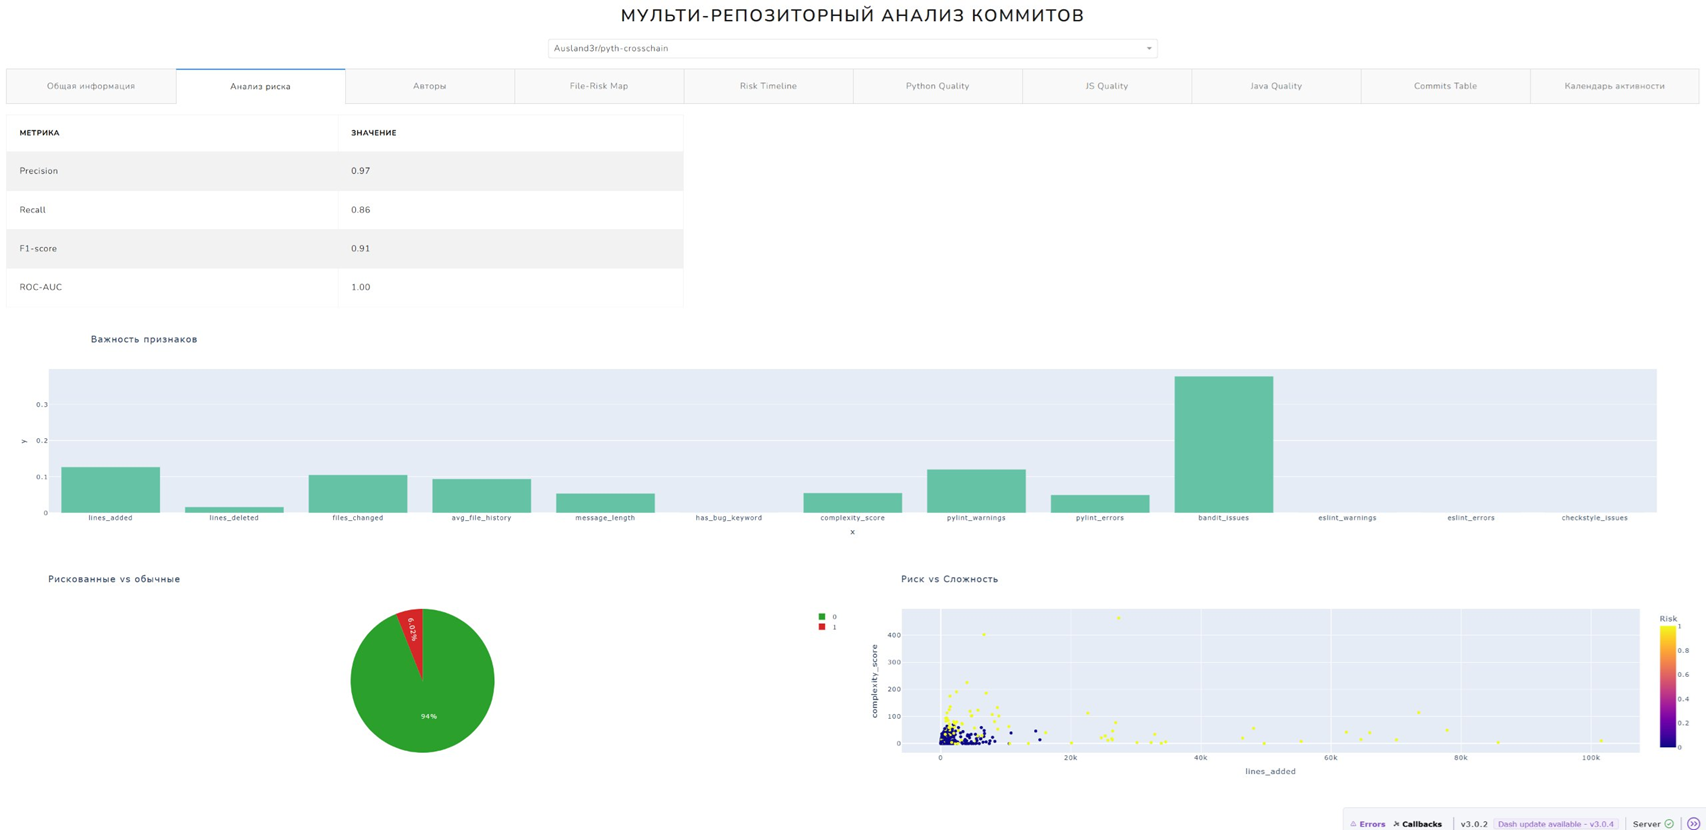
\includegraphics[width=\textwidth]{my_folder/images/nagruzka.png}
	\caption{Запущенная система с репозиторием \texttt{jup-ag/pyth-crosschain}}
	\label{tab:nagruzka}
\end{figure}

\section{Обзор и интерпретация результатов}
Визуализация результатов анализа коммитов позволяет быстро выявлять тенденции в проекте. Рассмотрим пример репозитория \texttt{Ausland3r/NTO2024-2025}. На рисунках приведены разные аспекты анализа:

Рисунок~\ref{fig:commit_stats} показывает гистограммы базовых метрик коммитов. Видно, что большинство коммитов содержит меньше 10 добавленных или удалённых строк, а также влияет не более чем на 5 файлов. Сложность изменений (четвёртый график) в большинстве случаев небольшая. Такие диаграммы позволяют визуально оценить, что значительная часть коммитов малых по размеру и сложности, что характерно для аккуратного ведения проекта. 

 \begin{figure}[H]
	\centering
	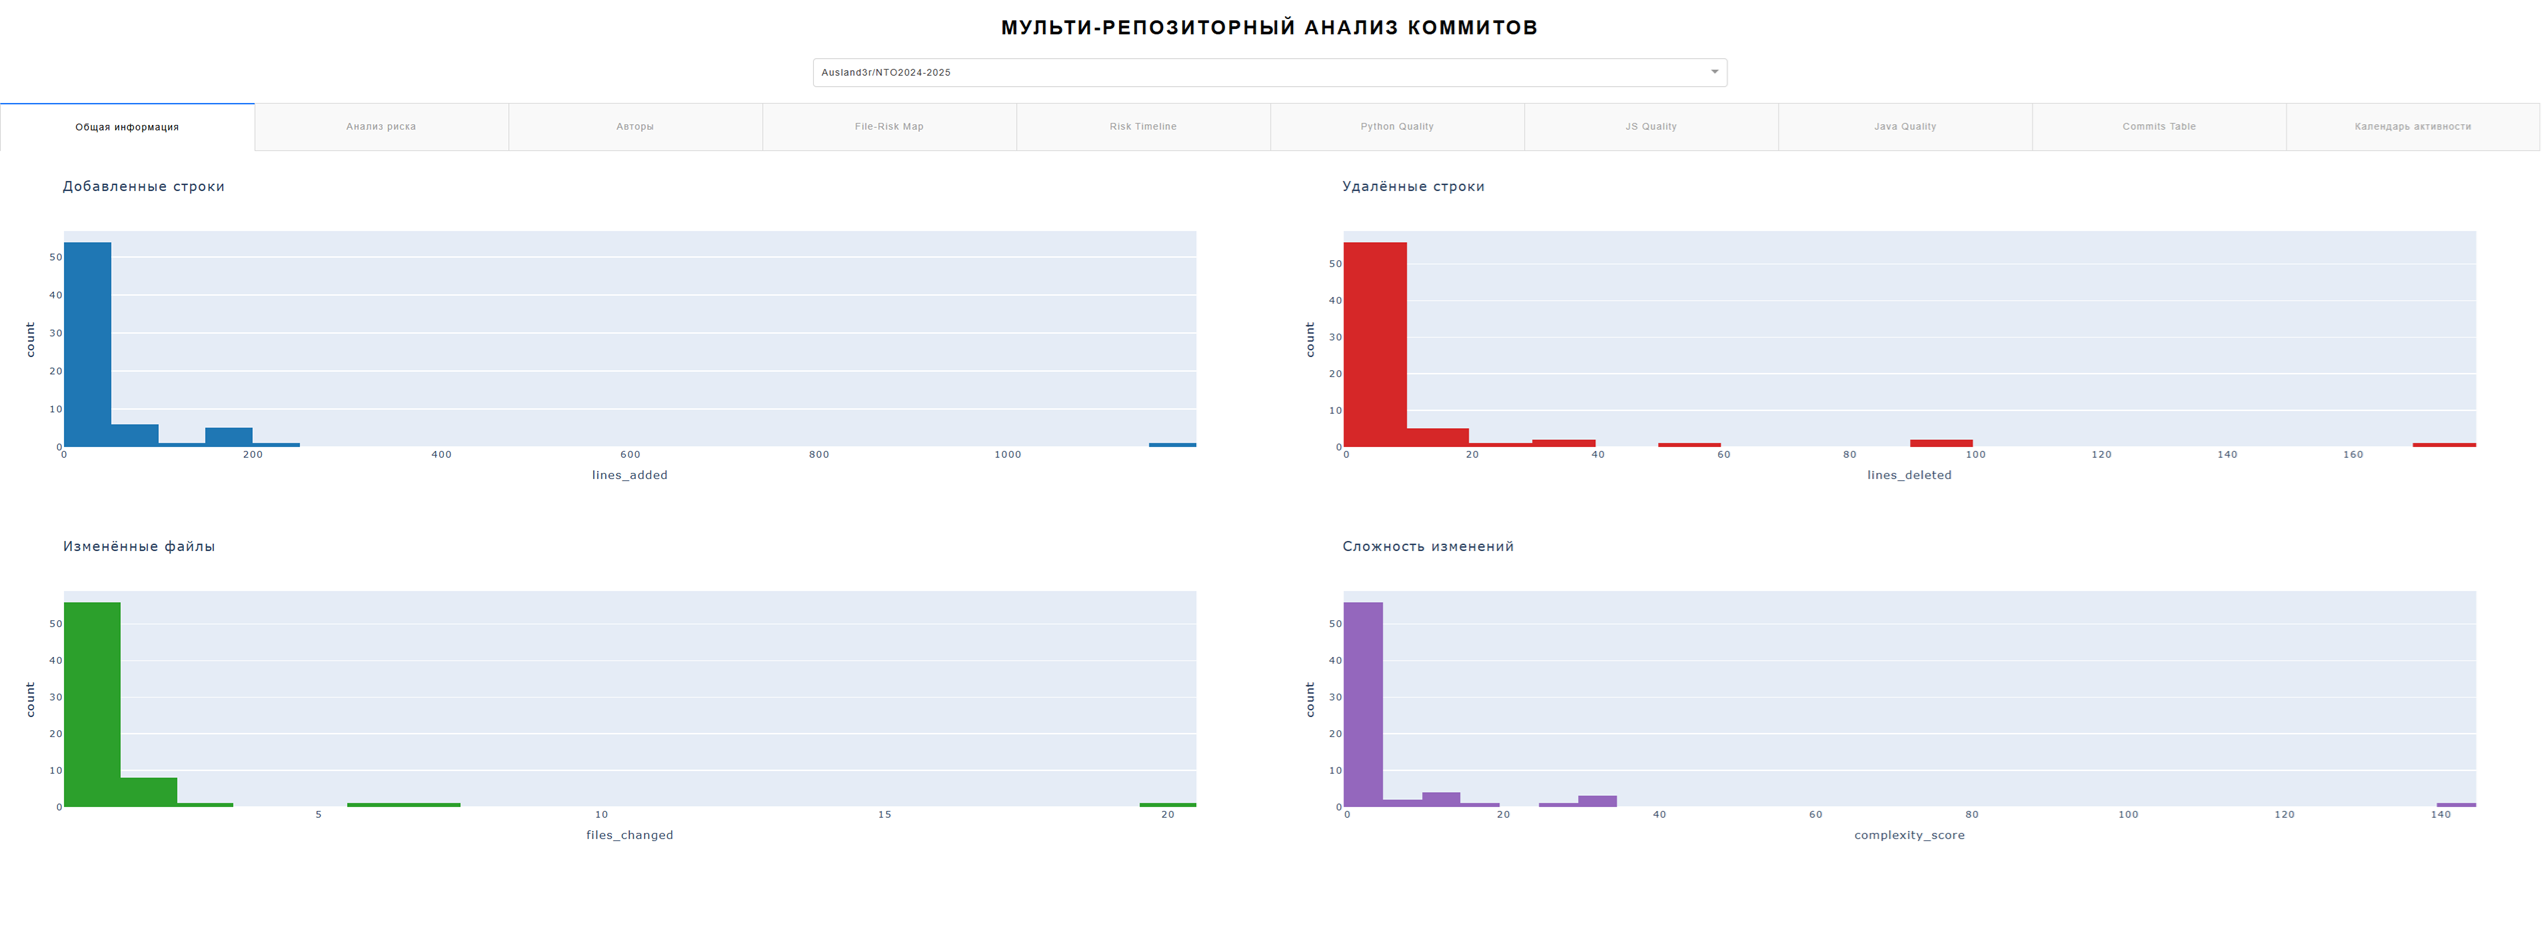
\includegraphics[width=\textwidth]{my_folder/images/first_page.png}
	\caption{Распределение изменений в коммитах: добавленные и удалённые строки, количество изменённых файлов и сложность изменений для проекта \texttt{Ausland3r/NTO2024-2025}.}
	\label{fig:commit_stats}
\end{figure}
На Рисунке~\ref{fig:risk_analysis} представлена информация об эффективности классификатора на этом репозитории. В таблице видим Precision=0.40, Recall=1.00, что соответствует метрикам модели на этих данных. Круговая диаграмма показывает, что около \verb|11.8%| коммитов отмечены как рисковые (красным цветом). Справа виден график «Risk vs Complexity»: наблюдается тенденция, что коммиты с большей сложностью имеют более высокий риск (жёлтым - рисковые коммиты). Данный анализ помогает подтвердить, что алгоритм верно выделяет несколько потенциально проблемных коммитов (в основном с большой сложностью), и диаграммы наглядно демонстрируют распределение рисковых изменений.

\begin{figure}[H]
	\centering
	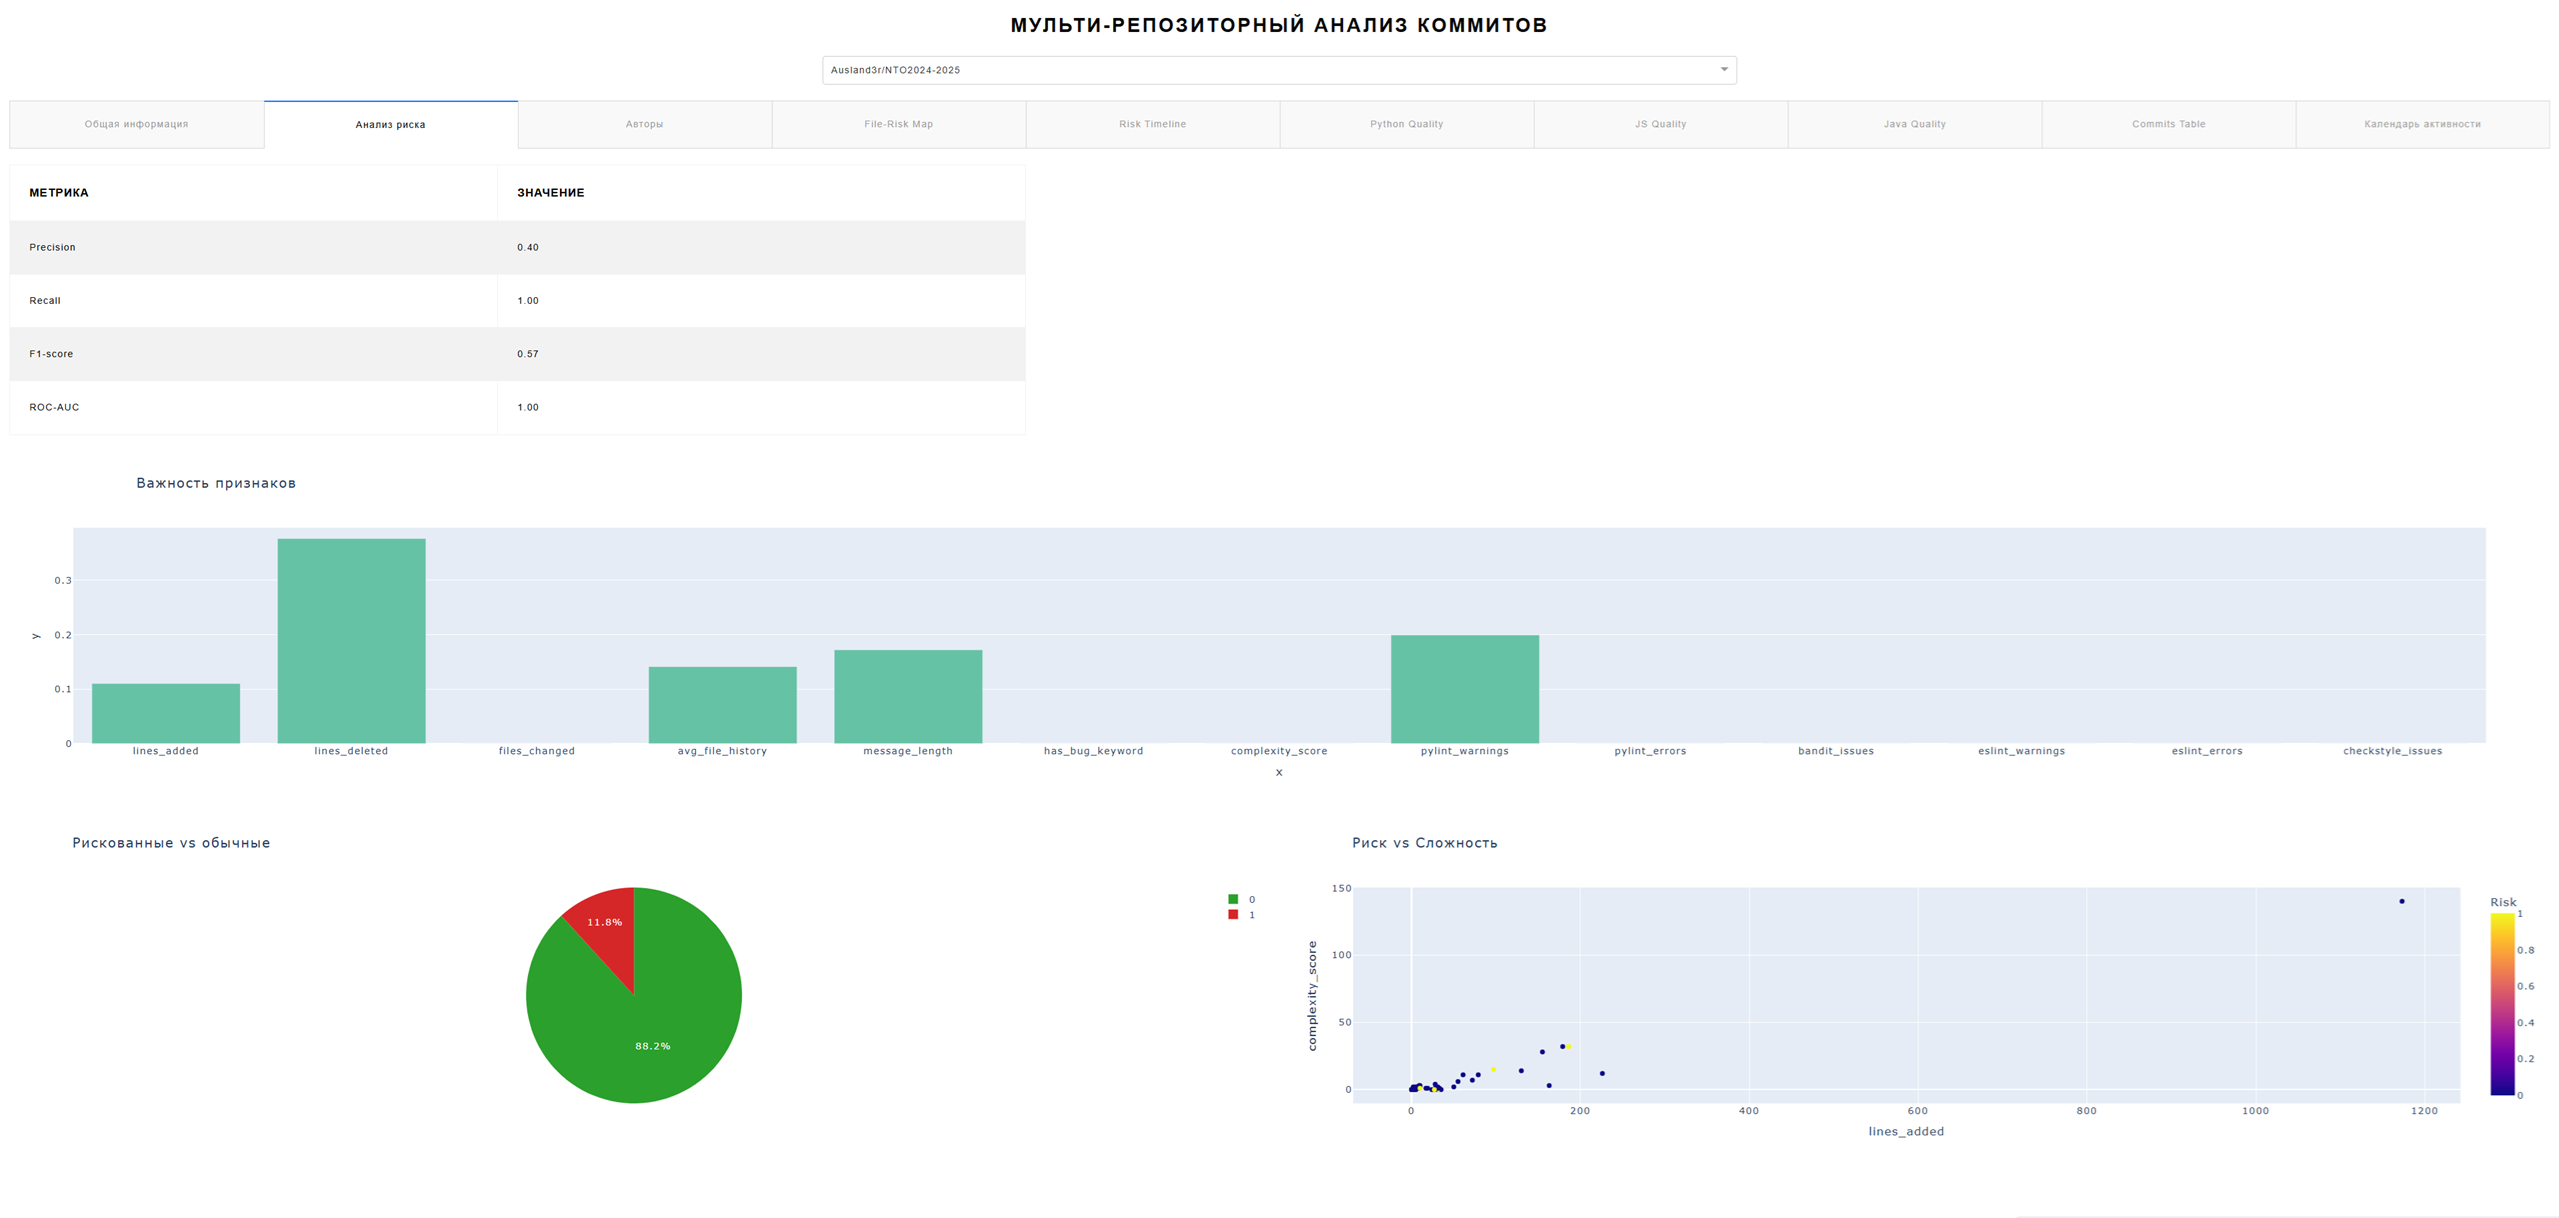
\includegraphics[width=\textwidth]{my_folder/images/second_page.png}
	\caption{Метрики классификации и распределение рисковых коммитов для репозитория \texttt{Ausland3r/NTO2024-2025}. Таблица показывает качество модели (Precision, Recall, F1, ROC-AUC), диаграмма слева — долю рисковых коммитов (красным), справа — зависимость риска от сложности.}
	\label{fig:risk_analysis}
\end{figure}

Рисунок~\ref{fig:authors} иллюстрирует вклад разных разработчиков. Слева видно, что основной объём коммитов внесли \texttt{Ausland3r} и \texttt{DenisovDmitrii} (по ~30 коммитов каждый), остальные авторы — единичные вклады. Справа график показывает средний риск по автору: например, \texttt{Fliegende\_Rehe} (средний риск ~0.4) выделяется как относительный «рисковый» автор, хотя у него было меньше коммитов. Такая визуализация помогает в определении, кто из участников при текущем анализе вносит больше потенциально проблемных изменений.

 \begin{figure}[ht]
	\centering
	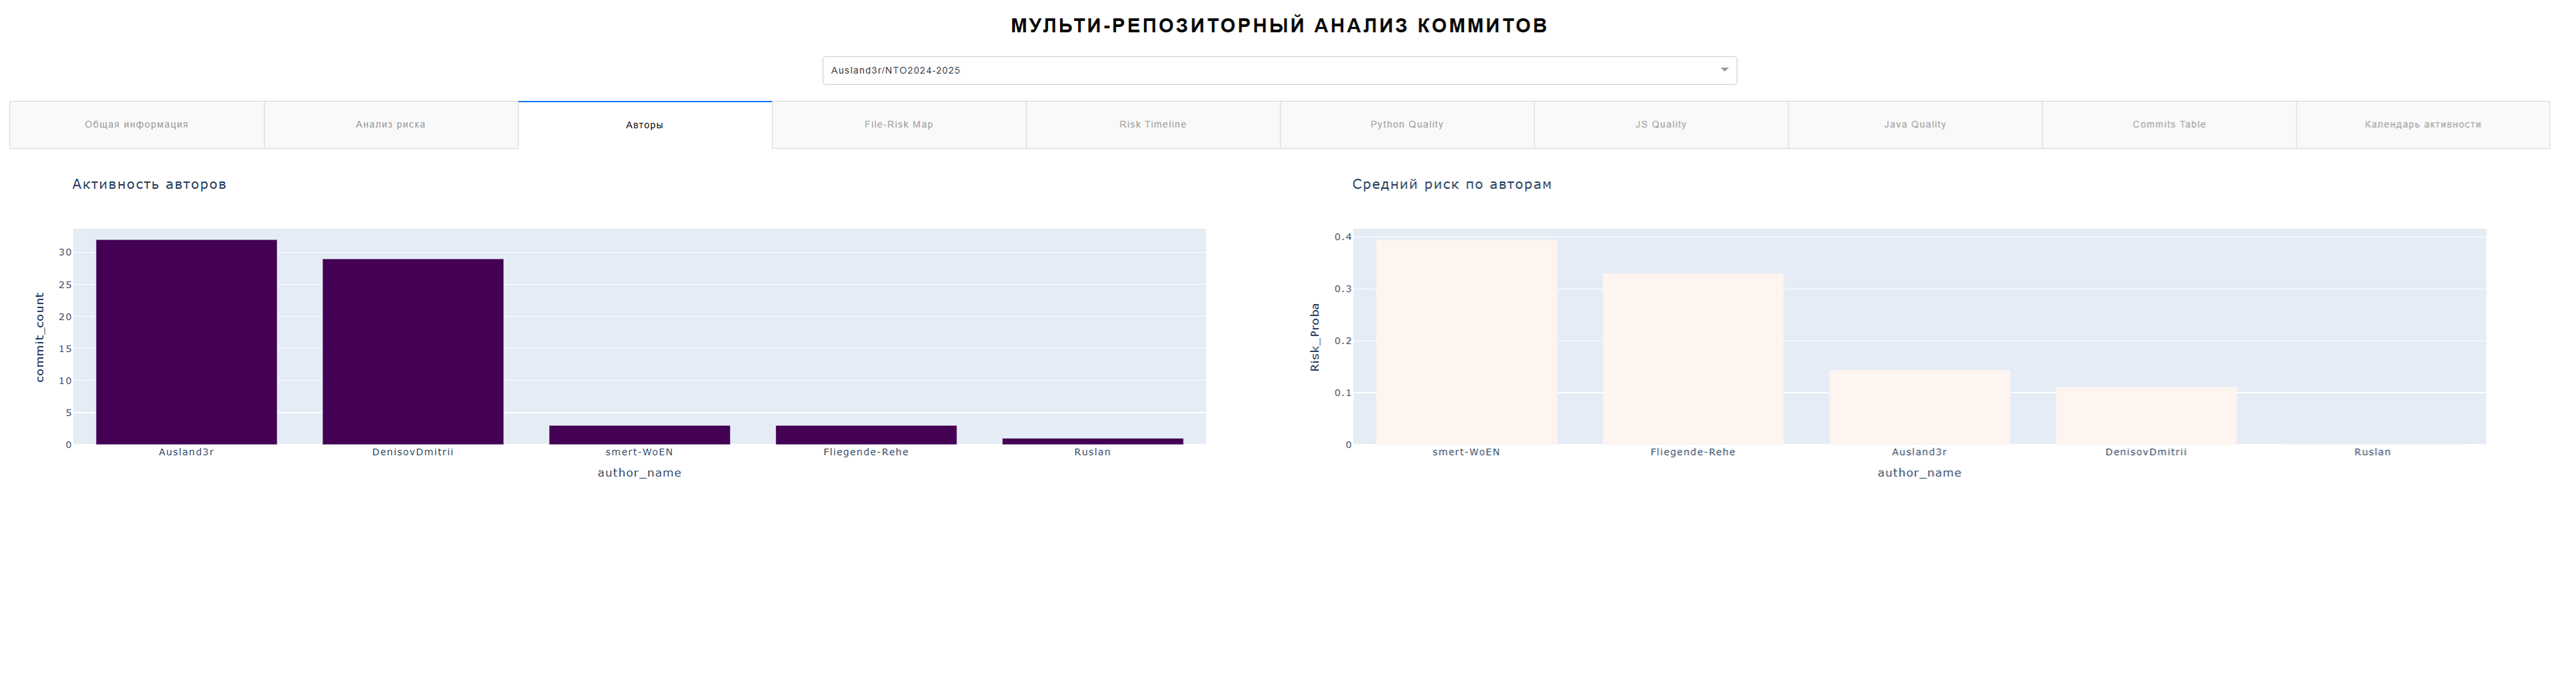
\includegraphics[width=\textwidth]{my_folder/images/third_page.png}
	\caption{Активность авторов и средний риск на автора для проекта \texttt{Ausland3r/NTO2024-2025}. Слева — число коммитов на автора, справа — усреднённый риск.}
	\label{fig:authors}
\end{figure}
 \begin{figure}[ht]
	\centering
	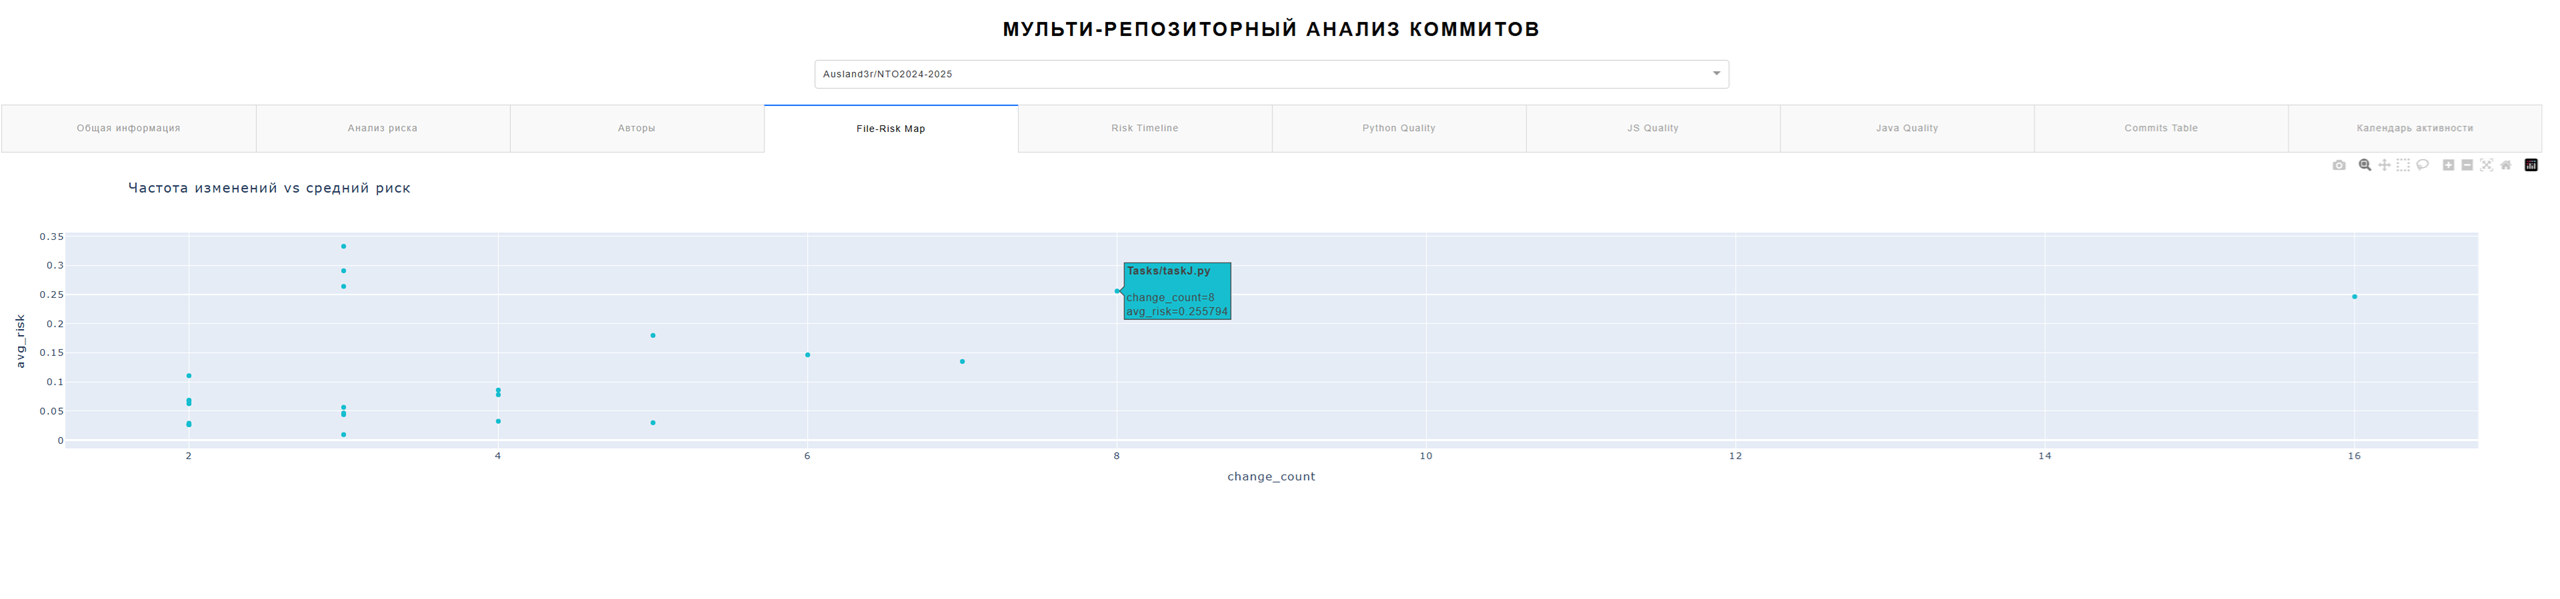
\includegraphics[width=\textwidth]{my_folder/images/forth_page.png}
	\caption{Файловая карта риска (частота изменений vs средний риск) для \texttt{Ausland3r/NTO2024-2025}. Точка \texttt{Task/taskJ.py} выделена как файл с 8 изменениями и средним риском 0.25.}
	\label{fig:file_risk}
\end{figure}

На Рисунке~\ref{fig:file_risk} представлена файловая карта: по горизонтали — число изменений файла (\texttt{change\_count}), по вертикали — средний риск изменений этого файла. Замечено, что файл \texttt{Task/task1.py} менялся 8 раз и имеет средний риск ~0.38 (отмечен на графике). Большинство же файлов имеют низкий риск. 

Такая диаграмма позволяет выявлять «горячие точки» проекта — файлы, часто изменяющиеся и с высоким риском, требующие внимания. 


Наконец, Рисунок~\ref{fig:timeline} демонстрирует динамику проекта. По синей линии видно, что средний риск коммитов постепенно рос с ноября 2024 по декабрь 2024. В мае 2025 на проекте снова были внесены изменения. Оранжевые столбцы отображают количество предупреждений статического анализа во времени. Видно несколько пиков предупреждений в начале проекта; далее они стабилизировались на низком уровне. Такая временная диаграмма подчёркивает, как со временем изменялась стабильность проекта, и позволяет своевременно заметить всплески риска или предупреждений. В целом приведённые визуализации показывают, что проект велся относительно аккуратно. 



\begin{figure}[ht]
	\centering
	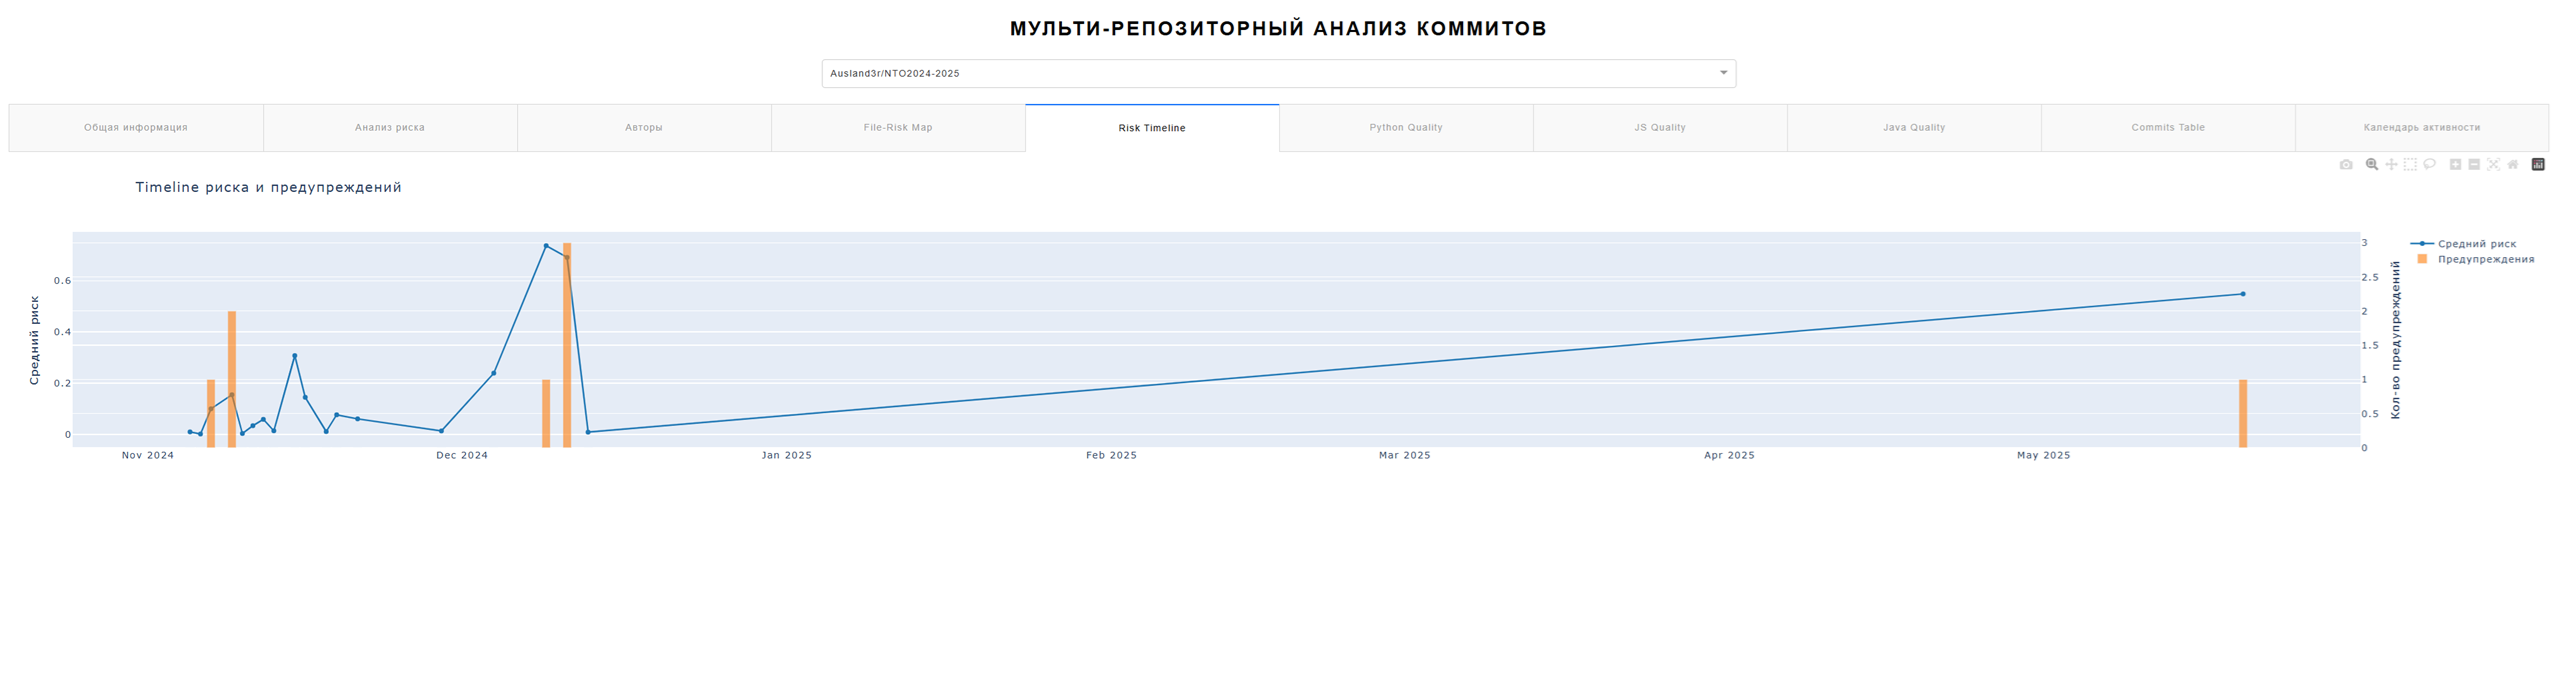
\includegraphics[width=\textwidth]{my_folder/images/fifth_page.png}
	\caption{Временная шкала риска и предупреждений для \texttt{Ausland3r/NTO2024-2025}. Синяя линия — средний риск коммитов с течением времени, оранжевые столбцы — число предупреждений статического анализа.}
	\label{fig:timeline}
\end{figure}

Визуальные представления, такие как вышеперечисленные, существенно упрощают анализ состояния проекта: они помогают быстро выделить проблемные области (рисковые коммиты, ответственные авторы, модифицируемые файлы и т.д.), которые трудно заметить при простом чтении логов. Аналитическая панель с такими графиками позволяет команде разработки эффективнее контролировать качество кода и прогнозировать потенциальные риски. 

\subsection{Описание страницы рекомендаций по коммитам}

На данной странице отображаются рекомендации по каждому коммиту репозитория, сгенерированные на основе анализа риска и метрик изменений. Рекомендации призваны помочь разработчикам и ревьюерам быстро оценить потенциальные проблемы и принять соответствующие меры.

\begin{figure}[ht]
	\centering
	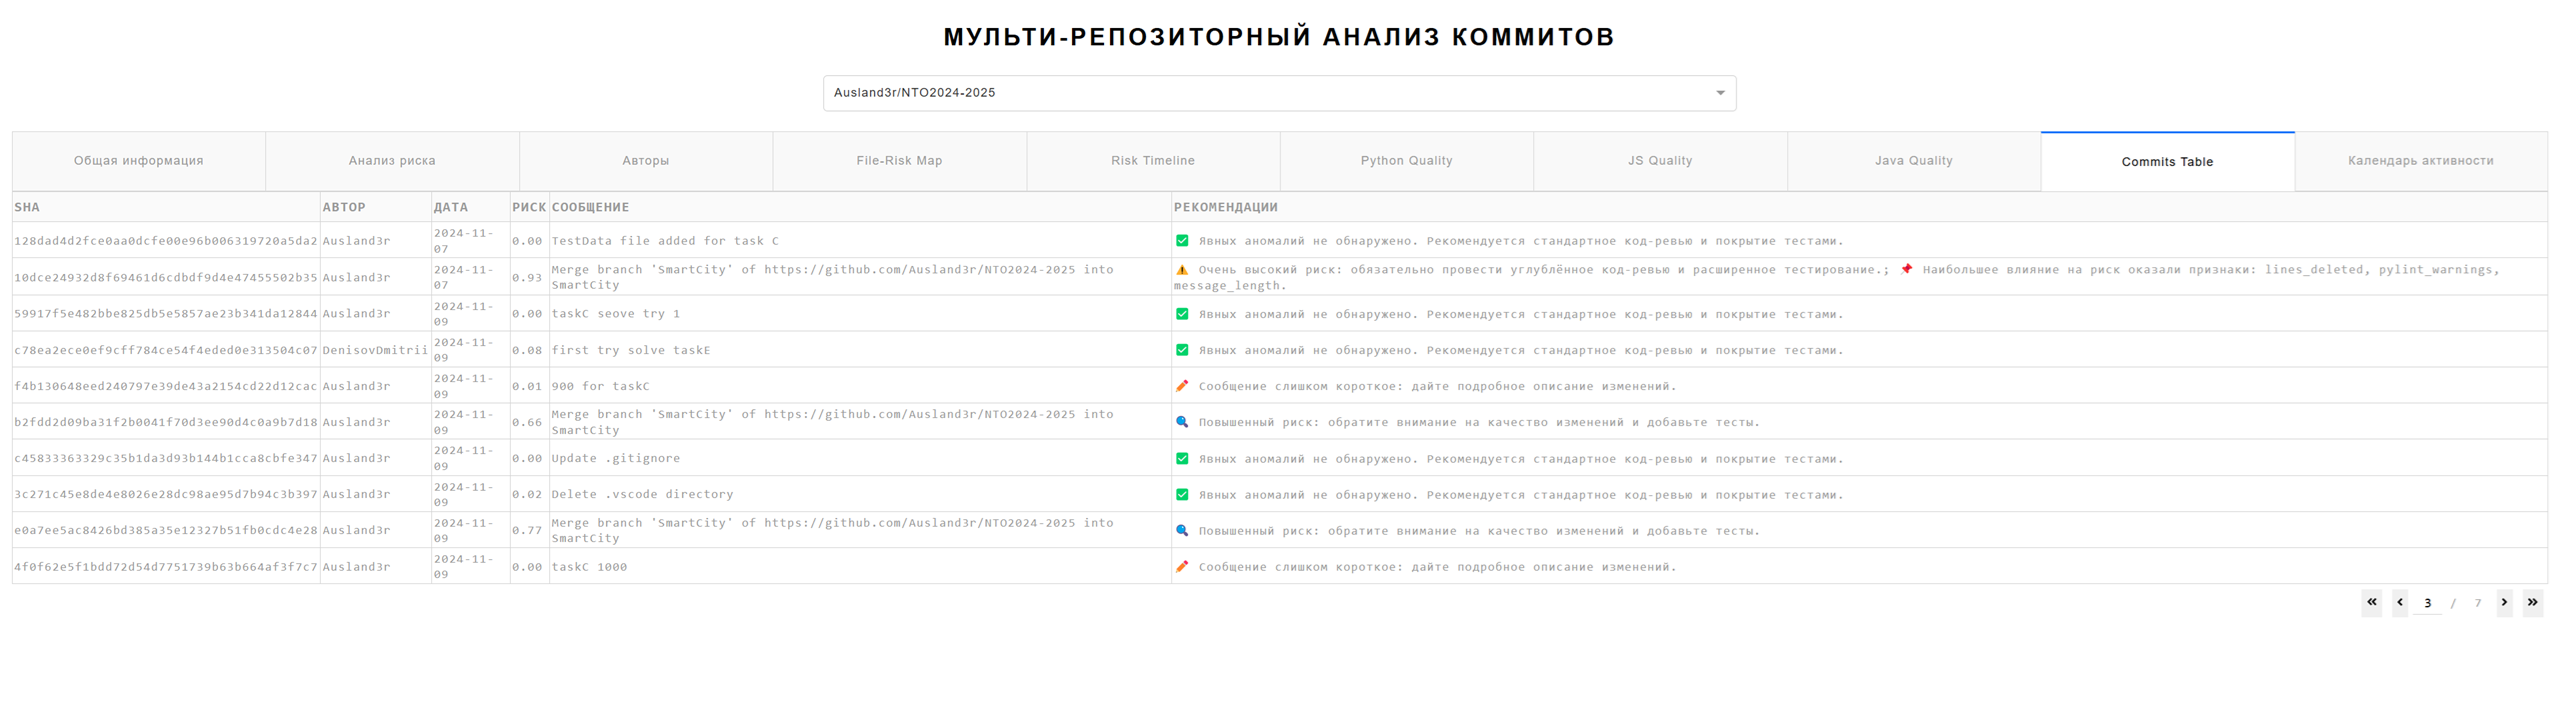
\includegraphics[width=\textwidth]{my_folder/images/capa_page.png}
	\caption{Таблица рисков и предупреждений для \texttt{Ausland3r/NTO2024-2025}.}
	\label{fig:timeline123}
\end{figure}

Основные виды рекомендаций включают:

\begin{itemize}
	\item Высокий риск (например, вероятность риска выше 0.8): 
	\begin{itemize}
		\item Рекомендуется углублённое код-ревью и расширенное тестирование.
		\item При наличии — показаны наиболее значимые признаки, повлиявшие на оценку риска, чтобы понять причины высокой оценки.
	\end{itemize}
	\item Повышенный риск (риск в диапазоне 0.5–0.8): 
	\begin{itemize}
		\item Совет обратить внимание на качество изменений и добавить тесты.
	\end{itemize}
	\item Качество сообщения коммита:
	\begin{itemize}
		\item Сообщения с длиной менее 15 символов получают рекомендацию расширить описание изменений.
		\item Очень длинные сообщения (более 200 символов) предлагается структурировать или сократить.
	\end{itemize}
	\item Объём изменений:
	\begin{itemize}
		\item Если количество изменённых строк значительно превышает среднее по репозиторию (свыше среднего плюс два стандартных отклонения), рекомендуется разбивать изменения на более мелкие логические части.
	\end{itemize}
	\item Специфические сигналы:
	\begin{itemize}
		\item Коммиты с ключевыми словами, указывающими на исправление багов, сопровождаются рекомендацией проверить наличие регрессионных тестов и обновление документации.
	\end{itemize}
\end{itemize}

Реализация рекомендаций основана на анализе различных метрик коммита, таких как длина сообщения, объём изменений, количество изменённых файлов, а также вероятности риска, вычисленные моделью. Это позволяет делать выводы не только на основе простых пороговых значений, но и учитывать специфику репозитория (через статистики по проекту) и значимость отдельных признаков риска.

Таким образом, представленные рекомендации реально соответствуют конкретному коммиту и его характеристикам, помогая в раннем выявлении потенциальных проблем и улучшении процесса код-ревью.

\vspace{0.5em}
Пример рекомендаций по коммиту:

\begin{quote}
	\begin{itemize}
		\item Очень высокий риск: обязательно провести углублённое код-ревью и расширенное тестирование.
		\item  Наибольшее влияние на риск оказали признаки: lines\_deleted, pylint\_warnings, message\_length.
		\item  Сообщение слишком короткое: дайте подробное описание изменений.
		\item Объём изменений (150) значительно превышает среднее (50.3). Разбейте коммит на более мелкие логические части.
	\end{itemize}
\end{quote}

Такая система рекомендаций повышает прозрачность оценки качества коммитов и способствует улучшению практик разработки в команде.

\section{Сравнение экспертных меток и рекомендаций, выданных моделью}

Для оценки качества работы системы по формированию рекомендаций и анализа рисковых коммитов были использованы экспертные метки, предоставленные опытными разработчиками из компаний \texttt{СТЦ} и \texttt{Coşkunöz Engineering and Tehnological Solutions}. Целью данного этапа тестирования было сравнить рекомендации, полученные с помощью модели \texttt{CommitRiskModel}, с теми, которые были предложены экспертами, и оценить, насколько хорошо модель воспроизводит их опыт и рекомендации.

Эксперты дали ряд рекомендаций по анализу сообщений коммитов и рисков, связанным с ними, в то время как модель предоставила свои собственные предложения на основе метрик, извлечённых из анализа репозиториев. В этом разделе будет проведено сравнение их выводов, а также проанализирована эффективность работы модели по сравнению с экспертными оценками.

\subsection{Рекомендации экспертов}

Экспертами были выделены несколько типов проблем, характерных для коммитов, с подробными рекомендациями по их улучшению:

\begin{itemize}
	\item Merge-коммиты: Эксперты отметили, что слияние веток через \texttt{merge} приводит к неудобствам при анализе истории изменений. Рекомендуется использовать методы слияния через \texttt{fast-forward} или \texttt{squash}, что улучшает читаемость истории коммитов и облегчает создание более понятных сообщений для merge-коммитов.
	\item Не-ASCII символы в сообщениях: Сообщения, содержащие не-ASCII символы, затрудняют использование стандартных инструментов, таких как \texttt{grep}, и могут привести к ошибкам при генерации чейнджлогов. Рекомендуется придерживаться единообразия в использовании символов, избегая нестандартных символов в сообщениях.
	\item Неатомарные изменения: Эксперты подчеркнули, что коммиты, которые затрагивают несколько логически несвязанных изменений, затрудняют понимание истории репозитория. Рекомендуется разделять такие изменения на несколько атомарных коммитов.
	\item Неинформативные сообщения: Сообщения, которые не раскрывают суть изменения, могут создать проблемы в будущем при анализе истории изменений. Рекомендуется предоставлять более подробные и описательные сообщения, которые точно объясняют изменения, внесённые в коммите.
	\item Невалидный автор коммита: Если автор и коммитер не совпадают, это может свидетельствовать о плохой организации работы с репозиторием и нарушении норм командной работы. Эксперты советуют избегать таких ситуаций, корректируя данные о коммитере.
	\item Наличие бинарных файлов в коммитах: Бинарные файлы, такие как \texttt{.zip}, \texttt{.pickle} и другие, могут создать проблемы при использовании системы контроля версий, поскольку их невозможно эффективно сравнивать или сливать. Эксперты рекомендуют избегать добавления бинарников в репозитории.
	\item Невыполнение стиля сообщений коммитов: Сообщения коммитов должны быть структурированы в соответствии с общепринятыми стандартами (например, \texttt{Conventional Commits}). Отсутствие контекста в сообщении коммита затрудняет точное понимание изменений и приводит к ухудшению документации в репозитории.
	\item Проверка наличия тестов: Эксперты рекомендуют обязательно добавлять тесты, если изменения касаются функционала.
	\item Частота коммитов: Частое сохранение прогресса важно и полезно, однако избыточные коммиты могут указывать на неаккуратную работу или спешку, что может привести к ухудшению качества кода и усложнить ревью. Эксперты рекомендуют делать менее частые, но более осмысленные и качественные коммиты.
\end{itemize}

\subsection{Рекомендации модели}

Модель \texttt{CommitRiskModel} предлагает рекомендации на основе анализа ряда факторов, таких как длина сообщения коммита, объём изменений, количество изменённых файлов, а также вероятность риска, вычисленная моделью. Некоторые ключевые рекомендации, выданные моделью, включают:

\begin{itemize}
	\item Сообщение коммита слишком короткое: если сообщение содержит менее 15 символов, рекомендуется предоставить более подробное описание.
	\item Объём изменений превышает среднее: если изменения значительно превышают средний объём для репозитория, модель предлагает разделить коммит на более мелкие логические части.
	\item Ключевые слова в сообщении: если коммит содержит ключевые слова, такие как "fix" или "bug", рекомендуется проверить наличие регрессионных тестов.
	\item Merge-коммиты: модель рекомендует использовать методы слияния \texttt{squash} или \texttt{fast-forward}, а также составить нормальные сообщения для merge.
	\item Неатомарные изменения: модель предлагает разделить такие изменения на несколько более мелких коммитов для улучшения читаемости.
\end{itemize}

Пример рекомендации от модели:

Очень высокий риск: обязательно провести углублённое код-ревью и расширенное тестирование. Наибольшее влияние на риск оказали признаки: \verb|lines_deleted|, \verb|pylint_warnings|, \verb|message_length|. Сообщение слишком короткое: дайте подробное описание изменений. Объём изменений (150) значительно превышает среднее (50.3). Разбейте коммит на более мелкие логические части.

\subsection{Сравнение рекомендаций экспертов и модели}

Для более детального анализа была составлена таблица, сравнивающая рекомендации, предложенные экспертами, с теми, что были выданы моделью:

\begin{table}[h!]
	\centering
	\caption{Сравнение рекомендаций экспертов и модели для репозитория Pacan4ik/tf-idf}
	\label{tab:expert_vs_model_recommendations}
	\small
	\begin{tabularx}{\textwidth}{|p{2.5cm}|X|X|}
		\hline
		\textbf{SHA коммита} & \textbf{Рекомендации эксперта} & \textbf{Рекомендации модели} \\
		\hline
		6aa0ac9, f9dba1c & Merge-коммиты лучше делать с использованием стандартных сообщений (например, squash или fast-forward) для удобства чтения истории. & Merge-коммиты, неудобно для анализа, рекомендуется использовать fast-forward или squash \\
		\hline
		ca6655a, 079146f & Сообщения содержат не-ASCII символы, улучшите читаемость & В сообщении обнаружены нестандартные символы. Желательно использовать только ASCII \\
		\hline
		6ad7d36, 838f481 & Неатомарные изменения, разделите на логически завершённые части & Неатомарные изменения, разделите на более мелкие, логически завершённые коммиты \\
		\hline
		ca6655a, f84a4db & Сообщение не раскрывает суть изменения, добавьте описание & Сообщение не несет смысла, добавьте подробное описание изменений \\
		\hline
		250fab4 & Несоответствие стилю сообщения коммита, улучшите форматирование & Сообщение очень короткое, пожалуйста, опишите изменения подробнее.\\
		\hline
		6ad7d36, 838f481 & Нарушение атомарности изменений, должны быть разделены & \makecell[tl]{Высокий риск: рекомендуется\\ провести детальный код-ревью.\\Основные факторы риска:\\ message\_length, files\_changed,\\ avg\_file\_history} \\
		\hline
		4e5660e, 0b7863b & Сообщение коммита без контекста, используйте стандарты & Сообщение не информативно, добавьте больше деталей о произведённых изменениях \\
		\hline
		196baa7, 7b707df & Отсутствие тестов для изменений & Добавьте тесты, чтобы подтвердить корректность изменений \\
		\hline
		05caf51, 7b707df & Несоответствие авторства коммита (author и committer разные) & Проверьте соответствие авторства и коммита, исправьте несоответствия \\
		\hline
		7404e85, 838f481 & Наличие бинарных файлов в коммите, что недопустимо для контроля версий & Удалите бинарные файлы из коммита. \\
		\hline
		250fab4, 4e5660e & Проблемы с форматированием сообщения коммита & Сообщение коммита слишком короткое, добавьте более подробное описание изменений \\
		\hline
		7b707df, 0b7863b & Несоответствие форматирования коммита, добавьте контекст & Сообщение слишком короткое, оно не даёт понимания изменений \\
		\hline
	\end{tabularx}
\end{table}

Из сравнения рекомендаций экспертов и модели можно сделать следующие выводы:

Модель предоставляет рекомендации, которые в большинстве случаев соответствуют экспертным меткам. Основные рекомендации, такие как использование fast-forward или squash для merge-коммитов, разделение неатомарных изменений и улучшение сообщений, совпадают.
Модель также выдает полезные предложения по улучшению качества сообщений и увеличению точности изменений, что подтверждает её эффективность в анализе репозиториев.
Несмотря на высокую степень совпадения, есть области, где модель могла бы быть улучшена, например, в более точном учете контекста изменений, что позволило бы избежать некоторых ложных срабатываний.

Система, в целом, эффективно предоставляет рекомендации, которые могут улучшить качество кода в проекте, обеспечив более строгие практики ведения репозиториев.

\section{Выводы}
В результате экспериментального тестирования подтверждена корректность реализации разработанной системы: интерфейс и функциональные блоки работают согласно заданию, а обученный классификатор рисковых коммитов показывает адекватные метрики на реальных данных. Успешно протестирована модель генерации рекомендаций CAPA: выявленные рекомендации соответствуют ожидаемым паттернам исправлений. Модульные тесты покрыли основные пути выполнения, включая граничные сценарии, что свидетельствует о надёжности кода. Нагрузочные тесты показали, что система масштабируема — даже при анализе тысячи коммитов реакция остаётся предсказуемой, хотя оптимизации статического анализа целесообразны для ускорения. Сильными сторонами подхода являются комплексность анализа (объединение статики кода, анализа коммитов и визуализации) и высокая адаптивность модели (универсальный класс классификатора позволяет легко тестировать новые алгоритмы). Подробные визуализации дают мощный инструмент мониторинга проекта. Возможные улучшения: расширение набора признаков за счёт динамических метрик (например, метрики сборки или покрытия тестами), а также использование реальных размеченных данных для обучения классификатора вместо эвристической псевдоразметки. При дальнейшем развитии можно добавить автоматические рекомендации по приоритетам исправлений на основе выявленных рисков. В целом, проведённое экспериментальное тестирование подтвердило, что разработанный подход позволяет эффективно выявлять и анализировать рисковые изменения в репозиториях, обеспечивая корректность работы системы и демонстрируя перспективу для дальнейшего улучшения инструментов разработки.           	 % Глава 3
\ContinueChapterEnd % завершить размещение глав <<подряд>>
%% Завершение основной части

\chapter*{Заключение} \label{ch-conclusion}
\addcontentsline{toc}{chapter}{Заключение} % в оглавление

В ходе данной работы была разработана система автоматического анализа коммитов, направленная на выявление аномалий и формирование корректирующих и предупреждающих действий (CAPA). Использование методов машинного обучения и кластеризации позволило создать инструмент, способный анализировать историю изменений в коде и предлагать рекомендации для повышения качества программного обеспечения.

Основные результаты работы можно сформулировать следующим образом:
\begin{itemize}
	\item Проведен обзор существующих методов анализа данных из репозиториев исходного кода и выявлены их ограничения.
	\item Разработан алгоритм автоматического извлечения данных о коммитах с последующей их обработкой и анализом.
	\item Предложен метод кластеризации коммитов с использованием алгоритма KMeans для определения пороговых значений изменений в коде.
	\item Обучены и протестированы модели машинного обучения (случайный лес, наивный байесовский классификатор и глубокий лес), показавшие высокую точность в задаче предсказания аномалий.
	\item Разработан механизм автоматического создания pull request с рекомендациями CAPA, который интегрируется в процесс разработки.
	\item Создан интерактивный дашборд для визуализации результатов анализа, что позволяет разработчикам легко отслеживать состояние репозитория и принимать решения на основе данных.
\end{itemize}

Практическая значимость предложенной системы заключается в том, что она позволяет автоматизировать контроль за качеством кода, минимизировать ошибки, возникающие в процессе разработки, и повысить прозрачность изменений в репозитории. Используемый подход может быть адаптирован для различных проектов и масштабируем для работы с крупными кодовыми базами.

В дальнейшем возможны следующие направления развития системы:
\begin{itemize}
	\item Доработка алгоритмов выявления аномалий с учетом более сложных паттернов изменений в коде.
	\item Расширение набора метрик для анализа коммитов.
	\item Интеграция с другими инструментами контроля качества кода и CI/CD системами.
	\item Применение нейросетевых моделей для улучшения предсказательной способности системы.
\end{itemize}

Таким образом, проведенное исследование подтвердило эффективность предложенного подхода к анализу коммитов. Разработанная система способствует улучшению управления процессом разработки программного обеспечения, сокращает время на выявление потенциальных проблем и повышает качество выпускаемого кода.


\chapter*{Приложение} \label{ch5}

\begin{lstlisting}[language=Python, caption={{ \texttt{repository\_analysis.py}}}]
	# repository_analysis.py
	
	import os
	import requests
	import re
	import json
	import subprocess
	from datetime import datetime
	import pandas as pd
	from git import Repo, GitCommandError
	from typing import List, Dict, Optional
	
	from xgboost import XGBClassifier
	
	from ml_model import CommitRiskModel
	from recommendations import generate_recommendations
	
	# mapping extension → analyzer name
	LANGUAGE_ANALYZERS = {
		'.py': 'python',
		'.js': 'javascript',
		'.ts': 'javascript',
		'.java': 'java',
	}
	
	class GitHubRepoAnalyzer:
	def __init__(
	self,
	repo_owner: str,
	repo_name: str,
	token: str,
	clone_dir: str = "/tmp",
	):
	self.repo_owner = repo_owner
	self.repo_name = repo_name
	self.token = token
	self.api_url = f"https://api.github.com/repos/{repo_owner}/{repo_name}"
	self.headers = {"Authorization": f"token {token}"}
	
	self.local_path = os.path.join(clone_dir, repo_name)
	if not os.path.isdir(self.local_path):
	clone_url = f"https://github.com/{repo_owner}/{repo_name}.git"
	print(f"[INIT] Cloning repository {clone_url} into {self.local_path}")
	Repo.clone_from(clone_url, self.local_path)
	print(f"[INIT] Clone complete.")
	else:
	print(f"[INIT] Repository already cloned at {self.local_path}.")
	self.repo = Repo(self.local_path)
	print(f"[INIT] Repo object ready at {self.local_path}.")
	
	self.complexity_re = re.compile(r"\b(if|for|while|switch|case)\b")
	
	def get_commits(self) -> List[Dict]:
	print("[COMMITS] Fetching commits via GitHub API")
	commits, page, per_page = [], 1, 100
	while True:
	print(f"[COMMITS] Requesting page {page}")
	resp = requests.get(
	f"{self.api_url}/commits",
	headers=self.headers,
	params={"page": page, "per_page": per_page},
	)
	data = resp.json()
	if resp.status_code == 401:
	raise RuntimeError("Bad credentials: check your GITHUB_TOKEN")
	if not isinstance(data, list):
	print(f"[COMMITS] Unexpected response: {data}")
	break
	commits.extend(data)
	print(f"[COMMITS] Retrieved {len(data)} commits in page {page}.")
	if len(data) < per_page:
	print(f"[COMMITS] Less than {per_page} commits on page {page}, finishing.")
	break
	page += 1
	print(f"[COMMITS] Total commits fetched: {len(commits)}")
	return commits
	
	def get_commit_details(self, sha: str) -> Dict:
	print(f"[DETAILS] Fetching details for commit {sha}")
	resp = requests.get(f"{self.api_url}/commits/{sha}", headers=self.headers)
	return resp.json()
	
	def detect_language(self, filename: str) -> str:
	_, ext = os.path.splitext(filename.lower())
	return LANGUAGE_ANALYZERS.get(ext, "")
	
	def analyze_python_file(self, full_path: str) -> Dict[str,int]:
	pyl_w = pyl_e = bandit = 0
	try:
	r = subprocess.run(
	["pylint", full_path, "--output-format=json"],
	stdout=subprocess.PIPE, stderr=subprocess.DEVNULL, text=True
	)
	msgs = json.loads(r.stdout or "[]")
	for m in msgs:
	if m.get("type") == "error":
	pyl_e += 1
	else:
	pyl_w += 1
	except Exception:
	print(f"[ANALYZE][PY] Pylint failed on {full_path}")
	try:
	r = subprocess.run(
	["bandit", "-f", "json", "-r", full_path],
	stdout=subprocess.PIPE, stderr=subprocess.DEVNULL, text=True
	)
	js = json.loads(r.stdout or "{}")
	bandit = len(js.get("results", []))
	except Exception:
	print(f"[ANALYZE][PY] Bandit failed on {full_path}")
	return {"pylint_warnings": pyl_w, "pylint_errors": pyl_e, "bandit_issues": bandit}
	
	def analyze_javascript_file(self, full_path: str) -> Dict[str,int]:
	w = e = 0
	try:
	r = subprocess.run(
	["eslint", full_path, "-f", "json"],
	stdout=subprocess.PIPE, stderr=subprocess.DEVNULL, text=True
	)
	arr = json.loads(r.stdout or "[]")
	for file_res in arr:
	for msg in file_res.get("messages", []):
	if msg.get("severity") == 2:
	e += 1
	else:
	w += 1
	except Exception:
	print(f"[ANALYZE][JS] ESLint failed on {full_path}")
	return {"eslint_warnings": w, "eslint_errors": e}
	
	def analyze_java_file(self, full_path: str) -> Dict[str,int]:
	count = 0
	try:
	r = subprocess.run(
	["checkstyle", "-f", "plain", full_path],
	stdout=subprocess.PIPE, stderr=subprocess.DEVNULL, text=True
	)
	for ln in r.stdout.splitlines():
	if "ERROR" in ln or "WARNING" in ln:
	count += 1
	except Exception:
	print(f"[ANALYZE][JAVA] Checkstyle failed on {full_path}")
	return {"checkstyle_issues": count}
	
	def compute_repo_stats(self, commits: List[Dict]) -> Dict:
	import pandas as pd
	df = pd.DataFrame(commits)
	stats = {}
	for f in ['lines_added', 'lines_deleted', 'files_changed',
	'avg_file_history', 'message_length', 'complexity_score']:
	if f in df:
	stats[f] = {
		'mean': df[f].mean(),
		'std': df[f].std(),
		'quantile_90': df[f].quantile(0.90),
		'quantile_95': df[f].quantile(0.95),
	}
	stats['author_stats'] = {a: {'median_lines_added': grp.median()}
		for a, grp in df.groupby('author_name')['lines_added']}
	if 'minutes_since_previous_commit' in df:
	stats['commit_interval'] = {'median': df['minutes_since_previous_commit'].median()}
	return stats
	
	def analyze_commits(self) -> List[Dict]:
	print("[ANALYZE]Starting commit-by-commit analysis")
	commits_data, file_count = [], {}
	
	all_commits = self.get_commits()
	all_commits.reverse()
	prev_dt = None
	
	for idx, c in enumerate(all_commits, 1):
	sha = c["sha"]
	print(f"[ANALYZE] ({idx}/{len(all_commits)}) Processing commit {sha}")
	det = self.get_commit_details(sha)
	
	try:
	print(f"[GIT] Checking out {sha}")
	self.repo.git.checkout(sha)
	except GitCommandError:
	print(f"[GIT] Cannot checkout {sha}, skipping FS analysis")
	
	msg = det["commit"]["message"]
	author = det["commit"]["author"]
	name = author.get("name", "Unknown")
	dt = datetime.strptime(author["date"], "%Y-%m-%dT%H:%M:%SZ")
	
	files = det.get("files", [])
	print(f"[ANALYZE]  {len(files)} files changed")
	
	added = sum(f.get("additions", 0) for f in files)
	deleted = sum(f.get("deletions", 0) for f in files)
	hist = sum(file_count.get(f["filename"], 0) for f in files)
	avg_hist = hist / len(files) if files else 0
	
	comp = 0
	for f in files:
	for ln in f.get("patch", "").splitlines():
	if ln.startswith("+") and not ln.startswith("+++") and self.complexity_re.search(ln):
	comp += 1
	
	delta = (dt - prev_dt).total_seconds() / 60 if prev_dt else None
	
	metrics = {k: 0 for k in (
		"pylint_warnings","pylint_errors","bandit_issues",
		"eslint_warnings","eslint_errors","checkstyle_issues"
		)}
	for f in files:
	lang = self.detect_language(f["filename"])
	full = os.path.join(self.local_path, f["filename"])
	if lang:
	print(f"[ANALYZE]Running {lang} analysis on {f['filename']}")
	if lang == "python":
	out = self.analyze_python_file(full)
	elif lang == "javascript":
	out = self.analyze_javascript_file(full)
	elif lang == "java":
	out = self.analyze_java_file(full)
	else:
	out = {}
	for k,v in out.items():
	metrics[k] += v
	
	data = {
		"commit": sha,
		"author_name": name,
		"author_datetime": dt,
		"minutes_since_previous_commit": delta,
		"message": msg,
		"message_length": len(msg),
		"lines_added": added,
		"lines_deleted": deleted,
		"files_changed": len(files),
		"avg_file_history": avg_hist,
		"complexity_score": comp,
		"file_list": [f["filename"] for f in files],
		**metrics
	}
	commits_data.append(data)
	
	for f in files:
	file_count[f["filename"]] = file_count.get(f["filename"], 0) + 1
	prev_dt = dt
	
	print(f"[ANALYZE] Completed analysis of {len(commits_data)} commits.")
	return commits_data
	
	def create_capa_file(self, commits: List[Dict]) -> str:
	path = os.path.join(self.local_path, "CapaRecommendations.md")
	with open(path, "w", encoding="utf-8") as f:
	f.write("CAPA Recommendations\n\n")
	for c in commits:
	if c.get("has_capa"):
	f.write(f"Commit {c['commit']} — risk={c['Risk_Proba']:.2f}\n")
	for rec in c["capa_recommendations"]:
	f.write(f"- {rec}\n")
	f.write("\n")
	return path
	
	def push_and_create_pr(self, branch_name: str, file_path: str) -> None:
	print(f"[PR] Fetching origin")
	self.repo.git.fetch('origin')
	
	base_branch = 'main'
	
	if branch_name in self.repo.branches:
	print(f"[PR] Branch {branch_name} already exists locally, checking out.")
	self.repo.git.checkout(branch_name)
	else:
	print(f"[PR] Creating branch {branch_name} from origin/{base_branch}")
	self.repo.git.checkout('-b', branch_name, f'origin/{base_branch}')
	
	rel_path = os.path.relpath(file_path, self.local_path)
	print(f"[PR] Adding file {rel_path}")
	self.repo.index.add([rel_path])
	print(f"[PR] Committing changes")
	self.repo.index.commit("Add CAPA recommendations")
	
	print(f"[PR] Pushing branch {branch_name}")
	origin = self.repo.remote(name='origin')
	origin.push(branch_name)
	
	pr_data = {
		"title": "Add automated CAPA recommendations",
		"head": f"{self.repo_owner}:{branch_name}",
		"base": base_branch,
		"body": "This PR adds automatically generated corrective/preventive actions."
	}
	print(f"[PR] Opening PR via GitHub API")
	response = requests.post(
	f"{self.api_url}/pulls",
	headers=self.headers,
	json=pr_data
	)
	if response.status_code in (200, 201):
	pr_url = response.json().get("html_url")
	print(f"[PR] Pull request created: {pr_url}")
	else:
	print(f"[PR]Failed to create PR: {response.status_code} {response.text}")
	
	def analyze_and_pr(self, commits: Optional[List[Dict]] = None) -> None:
	if commits is None:
	commits = self.analyze_commits()
	
	if not commits:
	print("No commits — пропускаем PR.")
	return
	
	model = CommitRiskModel(classifier=XGBClassifier(eval_metric="logloss"))
	model.fit(commits)
	probs = model.predict_proba(commits)
	
	repo_stats = self.compute_repo_stats(commits)
	
	for commit, p in zip(commits, probs):
	commit["Risk_Proba"] = float(p)
	commit["has_capa"] = True
	commit["capa_recommendations"] = generate_recommendations(
	commit, p, repo_stats, model.feature_importances()
	)
	
	md_path = self.create_capa_file(commits)
	branch = f"capa-{datetime.utcnow():%Y%m%d%H%M}"
	self.push_and_create_pr(branch, md_path)
\end{lstlisting}

\begin{lstlisting}[language=Python, caption={{ \texttt{ml\_model.py}}}]
	# ml_models.py
	from collections import Counter
	from typing import List, Dict, Any, Optional
	import numpy as np
	from deepforest import CascadeForestClassifier
	from sklearn.base import ClassifierMixin
	from sklearn.cluster import KMeans
	from sklearn.inspection import permutation_importance
	from sklearn.metrics import precision_score, recall_score, f1_score, roc_auc_score
	from sklearn.model_selection import train_test_split
	
	
	class CommitRiskModel:
	def __init__(
	self,
	classifier: ClassifierMixin,
	features: Optional[List[str]] = None,
	cluster_model: Optional[KMeans] = None
	):
	self.classifier = classifier
	self.features = features or [
	'lines_added', 'lines_deleted', 'files_changed',
	'avg_file_history', 'message_length',
	'has_bug_keyword', 'complexity_score'
	]
	self.cluster_model = cluster_model or KMeans(n_clusters=2, random_state=0, n_init=10)
	self._is_fitted = False
	self._X: Optional[np.ndarray] = None
	self._y: Optional[np.ndarray] = None
	
	def _extract_X(self, commits: List[Dict[str, Any]]) -> np.ndarray:
	return np.array([[commit.get(f, 0) for f in self.features] for commit in commits])
	
	def _generate_pseudo_labels(self, X: np.ndarray) -> np.ndarray:
	labels = self.cluster_model.fit_predict(X)
	centers = self.cluster_model.cluster_centers_
	
	dist0 = np.linalg.norm(X - centers[0], axis=1)
	dist1 = np.linalg.norm(X - centers[1], axis=1)
	
	prob_cluster1 = dist0 / (dist0 + dist1 + 1e-8)
	
	if centers[0, 0] > centers[1, 0]:
	prob_risky = 1 - prob_cluster1
	else:
	prob_risky = prob_cluster1
	
	threshold = 0.3
	labels_soft = (prob_risky >= threshold).astype(int)
	
	return labels_soft
	
	def fit(self, commits: List[Dict[str, Any]]):
	X = self._extract_X(commits)
	y = self._generate_pseudo_labels(X)
	self.classifier.fit(X, y)
	self._X, self._y = X, y
	self._is_fitted = True
	return self
	
	def predict(self, commits: List[Dict[str, Any]]) -> np.ndarray:
	assert self._is_fitted, "Модель не обучена"
	X = self._extract_X(commits)
	return self.classifier.predict(X)
	
	def predict_proba(self, commits: List[Dict[str, Any]]) -> np.ndarray:
	assert self._is_fitted, "Модель не обучена"
	X = self._extract_X(commits)
	return self.classifier.predict_proba(X)[:, 1]
	
	def feature_importances(self) -> Dict[str, float]:
	if not self._is_fitted or self._X is None or self._y is None:
	raise RuntimeError("Нужно вызвать .fit() перед feature_importances()")
	if hasattr(self.classifier, "feature_importances_"):
	vals = self.classifier.feature_importances_
	else:
	result = permutation_importance(
	self.classifier, self._X, self._y,
	n_repeats=5, random_state=0, n_jobs=-1
	)
	vals = result.importances_mean
	return dict(zip(self.features, vals))
	
	def evaluate_model(self, commits: List[Dict[str, Any]]) -> Dict[str, float]:
	X = self._extract_X(commits)
	y = self._generate_pseudo_labels(X)
	print("[DEBUG] Метки (y) распределение:", Counter(y))
	
	if len(set(y)) < 2:
	print("[WARNING] В данных только один класс, метрики классификации не применимы.")
	clf = self.classifier
	clf.fit(X, y)
	y_pred = clf.predict(X)
	y_proba = clf.predict_proba(X)[:, 1] if hasattr(clf, "predict_proba") else np.zeros_like(y_pred,
	dtype=float)
	return {
		"precision": 0.0,
		"recall": 0.0,
		"f1_score": 0.0,
		"auc": 0.0
	}
	
	stratify_param = y if min(Counter(y).values()) > 1 else None
	X_train, X_test, y_train, y_test = train_test_split(
	X, y, test_size=0.2, random_state=42, stratify=stratify_param
	)
	
	if isinstance(self.classifier, CascadeForestClassifier):
	clf = CascadeForestClassifier(random_state=42)
	else:
	from copy import deepcopy
	clf = deepcopy(self.classifier)
	
	clf.fit(X_train, y_train)
	y_pred = clf.predict(X_test)
	print("[DEBUG] y_pred распределение:", Counter(y_pred))
	
	if hasattr(clf, "predict_proba"):
	y_proba = clf.predict_proba(X_test)[:, 1]
	print("[DEBUG] y_proba min/max:", y_proba.min(), y_proba.max())
	else:
	y_proba = np.zeros_like(y_pred, dtype=float)
	
	precision = precision_score(y_test, y_pred, zero_division=0)
	recall = recall_score(y_test, y_pred, zero_division=0)
	f1 = f1_score(y_test, y_pred, zero_division=0)
	auc = roc_auc_score(y_test, y_proba) if len(set(y_test)) == 2 else 0.0
	
	return {
		"precision": precision,
		"recall": recall,
		"f1_score": f1,
		"auc": auc
	}
\end{lstlisting}

\begin{lstlisting}[language=Python, caption={{ \texttt{app.py}}}]
	# app.py
	
	import os
	from dotenv import load_dotenv
	import dash
	from dash import dcc, html, dash_table
	from dash.dependencies import Input, Output
	import dash_bootstrap_components as dbc
	import plotly.express as px
	import plotly.graph_objects as go
	import pandas as pd
	import numpy as np
	
	from repository_analysis import GitHubRepoAnalyzer
	from ml_model import CommitRiskModel
	from xgboost import XGBClassifier
	from deepforest import CascadeForestClassifier
	from recommendations import generate_recommendations
	
	# 1. Загрузка настроек
	load_dotenv()
	github_token = os.getenv('GITHUB_TOKEN')
	repos = [r for r in os.getenv("GITHUB_REPOS", "").split(",") if r]
	
	# 2. Сбор и анализ каждого репозитория
	analyses = {}
	for full_name in repos:
	owner, name = full_name.split("/")
	analyzer = GitHubRepoAnalyzer(owner, name, github_token)
	commits = analyzer.analyze_commits()
	analyzer.analyze_and_pr(commits)
	
	# 3. Обучение модели на коммитах
	#model = CommitRiskModel(XGBClassifier(eval_metric="logloss"))
	model = CommitRiskModel(CascadeForestClassifier(random_state=42))
	model.fit(commits)
	metrics = model.evaluate_model(commits)
	
	# 4. Подготовка DataFrame
	df = pd.DataFrame(commits)
	df['Risk_Proba'] = model.predict_proba(commits)
	df['Risk'] = (df['Risk_Proba'] > 0.5).astype(int)
	
	analyses[full_name] = {
		'df': df,
		'model': model,
		'feat_imps': model.feature_importances(),
		'metrics': metrics
	}
	
	# 5. Инициализация Dash-приложения
	app = dash.Dash(__name__, external_stylesheets=[dbc.themes.LUX])
	
	app.layout = dbc.Container(fluid=True, children=[
	html.H1("Мульти-репозиторный анализ коммитов", className="text-center my-4"),
	dcc.Dropdown(
	id="repo-selector",
	options=[{"label": r, "value": r} for r in repos],
	value=repos[0] if repos else None,
	clearable=False,
	style={"width": "60%", "margin": "0 auto 20px auto"}
	),
	html.Div(id="tabs-container")
	])
	
	@app.callback(
	Output("tabs-container", "children"),
	Input("repo-selector", "value")
	)
	def update_tabs(selected_repo):
	if not selected_repo or selected_repo not in analyses:
	return html.Div("Репозиторий не выбран или недоступен")
	
	entry = analyses[selected_repo]
	df = entry['df'].copy()
	feat_imps = entry['feat_imps']
	metrics = entry.get('metrics', {})
	metrics_table = dbc.Table([
	html.Thead(html.Tr([html.Th("Метрика"), html.Th("Значение")])),
	html.Tbody([
	html.Tr([html.Td("Precision"), html.Td(f"{metrics.get('precision', 0):.2f}")]),
	html.Tr([html.Td("Recall"), html.Td(f"{metrics.get('recall', 0):.2f}")]),
	html.Tr([html.Td("F1-score"), html.Td(f"{metrics.get('f1_score', 0):.2f}")]),
	html.Tr([html.Td("ROC-AUC"), html.Td(f"{metrics.get('auc', 0):.2f}")]),
	])
	], bordered=True, striped=True, hover=True, style={"width": "40%", "marginTop": "20px"})
	features = entry['model'].features
	
	# Подстраховки
	if 'author_name' not in df:
	df['author_name'] = 'Unknown'
	if 'has_bug_keyword' not in df:
	df['has_bug_keyword'] = df['message'].str.contains(
	r'\b(fix|bug|error)\b', case=False, regex=True, na=False
	).astype(int)
	
	# 6. Общая информация
	tab_summary = dcc.Tab(label='Общая информация', children=[
	dbc.Row([
	dbc.Col(dcc.Graph(
	figure=px.histogram(
	df, x='lines_added', nbins=30,
	title='Добавленные строки',
	color_discrete_sequence=['#1f77b4']  # синяя
	)
	), md=6),
	dbc.Col(dcc.Graph(
	figure=px.histogram(
	df, x='lines_deleted', nbins=30,
	title='Удалённые строки',
	color_discrete_sequence=['#d62728']  # красная
	)
	), md=6),
	], className="g-4"),
	dbc.Row([
	dbc.Col(dcc.Graph(
	figure=px.histogram(
	df, x='files_changed', nbins=30,
	title='Изменённые файлы',
	color_discrete_sequence=['#2ca02c']  # зелёная
	)
	), md=6),
	dbc.Col(dcc.Graph(
	figure=px.histogram(
	df, x='complexity_score', nbins=30,
	title='Сложность изменений',
	color_discrete_sequence=['#9467bd']  # фиолетовая
	)
	), md=6),
	], className="g-4"),
	])
	
	# 7. Анализ риска
	fi_vals = [feat_imps.get(f, 0) for f in features]
	tab_risk = dcc.Tab(label='Анализ риска', children=[
	metrics_table,
	dbc.Row(dbc.Col(dcc.Graph(
	figure=px.bar(
	x=features, y=fi_vals,
	title='Важность признаков',
	color_discrete_sequence=px.colors.qualitative.Set2
	)
	)), className="g-4"),
	dbc.Row([
	dbc.Col(dcc.Graph(
	figure=px.pie(
	df, names='Risk', title='Рискованные vs обычные',
	color_discrete_sequence=['#2ca02c', '#d62728']
	)
	), md=6),
	dbc.Col(dcc.Graph(
	figure=px.scatter(
	df, x='lines_added', y='complexity_score',
	color='Risk', title='Риск vs Сложность',
	color_discrete_sequence=['#2ca02c', '#d62728']
	)
	), md=6),
	], className="g-4"),
	])
	
	# 8. Авторы
	author_activity = df['author_name'].value_counts().reset_index()
	author_activity.columns = ['author_name', 'commit_count']
	author_risk = df.groupby('author_name')['Risk_Proba'] \
	.mean().reset_index() \
	.sort_values('Risk_Proba', ascending=False)
	
	tab_authors = dcc.Tab(label='Авторы', children=[
	dbc.Row([
	dbc.Col(dcc.Graph(
	figure=px.bar(
	author_activity, x='author_name', y='commit_count',
	title='Активность авторов',
	color_discrete_sequence=px.colors.sequential.Viridis
	)
	), md=6),
	dbc.Col(dcc.Graph(
	figure=px.bar(
	author_risk, x='author_name', y='Risk_Proba',
	title='Средний риск по авторам',
	color_discrete_sequence=px.colors.sequential.Reds
	)
	), md=6),
	], className="g-4"),
	])
	
	# 9. File-Risk Map
	file_df = df.explode('file_list') if 'file_list' in df else pd.DataFrame()
	if not file_df.empty:
	fr = file_df.groupby('file_list').agg(
	change_count=('file_list','size'),
	avg_risk=('Risk_Proba','mean')
	).reset_index()
	else:
	fr = pd.DataFrame(columns=['file_list','change_count','avg_risk'])
	tab_file_risk = dcc.Tab(label='File-Risk Map', children=[
	dbc.Row(dbc.Col(dcc.Graph(
	figure=px.scatter(
	fr, x='change_count', y='avg_risk',
	hover_name='file_list',
	title='Частота изменений vs средний риск',
	color_discrete_sequence=['#17becf']  # бирюзовая
	)
	)), className="g-4")
	])
	
	# 10. Risk Timeline
	df['commit_date'] = pd.to_datetime(df['author_datetime'], errors='coerce').dt.date
	tl = df.sort_values('commit_date').groupby('commit_date').agg(
	daily_risk=('Risk_Proba','mean'),
	warnings=('Risk','sum')
	).reset_index()
	fig_tl = go.Figure([
	go.Scatter(
	x=tl['commit_date'], y=tl['daily_risk'],
	mode='lines+markers', name='Средний риск',
	line=dict(color='#1f77b4')
	),
	go.Bar(
	x=tl['commit_date'], y=tl['warnings'],
	name='Предупреждения', yaxis='y2', opacity=0.6,
	marker_color='#ff7f0e'
	)
	])
	fig_tl.update_layout(
	title='Timeline риска и предупреждений',
	yaxis=dict(title='Средний риск'),
	yaxis2=dict(title='Кол-во предупреждений', overlaying='y', side='right')
	)
	tab_timeline = dcc.Tab(label='Risk Timeline', children=[
	dbc.Row(dbc.Col(dcc.Graph(figure=fig_tl)), className="g-4")
	])
	
	# 11. Code Quality Tabs
	quality_tabs = []
	if {'pylint_warnings','pylint_errors','bandit_issues'} <= set(df.columns):
	quality_tabs.append(dcc.Tab(label='Python Quality', children=[
	dbc.Row([
	dbc.Col(dcc.Graph(
	figure=px.histogram(
	df, x='pylint_warnings',
	title='Pylint Warnings',
	color_discrete_sequence=['#9467bd']
	)
	), md=6),
	dbc.Col(dcc.Graph(
	figure=px.scatter(
	df, x='pylint_errors', y='bandit_issues',
	title='Errors vs Security Issues',
	color_discrete_sequence=['#8c564b']
	)
	), md=6),
	], className="g-4")
	]))
	if {'eslint_warnings','eslint_errors'} <= set(df.columns):
	quality_tabs.append(dcc.Tab(label='JS Quality', children=[
	dbc.Row([
	dbc.Col(dcc.Graph(
	figure=px.histogram(
	df, x='eslint_warnings',
	title='ESLint Warnings',
	color_discrete_sequence=['#e377c2']
	)
	), md=6),
	dbc.Col(dcc.Graph(
	figure=px.scatter(
	df, x='eslint_errors', y='eslint_warnings',
	title='Errors vs Warnings',
	color_discrete_sequence=['#7f7f7f']
	)
	), md=6),
	], className="g-4")
	]))
	if 'checkstyle_issues' in df.columns:
	quality_tabs.append(dcc.Tab(label='Java Quality', children=[
	dbc.Row(dbc.Col(dcc.Graph(
	figure=px.histogram(
	df, x='checkstyle_issues',
	title='Checkstyle Issues',
	color_discrete_sequence=['#bcbd22']
	)
	)), className="g-4")
	]))
	
	# 12. Commits Table
	df['Recommendations'] = df.apply(
	lambda row: generate_recommendations(row, row['Risk_Proba'], {}, feat_imps),
	axis=1
	)
	df['Recommendations_Text'] = df['Recommendations'].apply(lambda recs: "; ".join(recs))
	tab_table = dcc.Tab(label='Commits Table', children=[
	dash_table.DataTable(
	columns=[
	{"name":"SHA","id":"commit"},
	{"name":"Автор","id":"author_name"},
	{"name":"Дата","id":"commit_date"},
	{"name":"Риск","id":"Risk_Proba","type":"numeric","format":{"specifier":".2f"}},
	{"name":"Сообщение","id":"message"},
	{"name":"Рекомендации","id":"Recommendations_Text"},
	],
	data=df[['commit','author_name','commit_date','Risk_Proba','message','Recommendations_Text']]
	.to_dict('records'),
	page_size=10,
	style_cell={'textAlign':'left','whiteSpace':'normal','height':'auto'},
	style_header={'fontWeight':'bold'}
	)
	])
	
	# 13. Календарь активности
	all_dates = pd.date_range(df['commit_date'].min(), df['commit_date'].max(), freq='D')
	heat = pd.DataFrame({'date': all_dates})
	heat['count'] = heat['date'].map(df['commit_date'].value_counts()).fillna(0)
	heat['dow'] = heat['date'].dt.weekday
	heat['week'] = ((heat['date'] - heat['date'].min()).dt.days // 7).astype(int)
	max_w = heat['week'].max() + 1
	mat = np.zeros((7, max_w))
	for _, r in heat.iterrows():
	mat[int(r['dow']), int(r['week'])] = r['count']
	cal_fig = go.Figure(data=go.Heatmap(
	z=mat,
	x=[f'Неделя {i+1}' for i in range(max_w)],
	y=['Пн','Вт','Ср','Чт','Пт','Сб','Вс'],
	colorscale='Greens', hoverongaps=False,
	colorbar=dict(title='Коммитов/день')
	))
	cal_fig.update_layout(xaxis=dict(scaleanchor='y', showgrid=False),
	yaxis=dict(showgrid=False))
	tab_calendar = dcc.Tab(label='Календарь активности', children=[
	dbc.Row(dbc.Col(dcc.Graph(figure=cal_fig)), className="g-4")
	])
	
	tabs = [
	tab_summary,
	tab_risk,
	tab_authors,
	tab_file_risk,
	tab_timeline,
	*quality_tabs,
	tab_table,
	tab_calendar
	]
	return dcc.Tabs(tabs)
	
	if __name__ == '__main__':
	app.run(debug=True)
\end{lstlisting}

\begin{lstlisting}[language=Python, caption={{ \texttt{recommendationds.py}}}]
	# recommendations.py
	from typing import List
	
	__all__ = ['generate_recommendations']
	
	def generate_recommendations(commit: dict,
	risk_proba: float,
	repo_stats: dict,
	feature_importances: dict) -> List[str]:
	
	recommendations: List[str] = []
	
	if risk_proba > 0.8:
	recommendations.append(
	"Очень высокий риск: обязательно провести углублённое код-ревью и расширенное тестирование."
	)
	elif risk_proba > 0.5:
	recommendations.append(
	"Повышенный риск: обратите внимание на качество изменений и добавьте тесты."
	)
	
	msg_len = commit.get('message_length', 0)
	if msg_len < 20:
	recommendations.append(
	"Сообщение слишком короткое: дайте подробное описание изменений."
	)
	elif msg_len > 200:
	recommendations.append(
	"Очень длинное сообщение: разделите описание на ключевые пункты или используйте более лаконичные формулировки."
	)
	
	if commit.get('has_bug_keyword', 0):
	recommendations.append(
	"Выявлен багфикс: убедитесь в наличии регрессионных тестов и обновлении документации."
	)
	
	lines_added = commit.get('lines_added', 0)
	lines_deleted = commit.get('lines_deleted', 0)
	total = lines_added + lines_deleted
	stats_total = repo_stats.get('total_changes', {})
	mean_total = stats_total.get('mean')
	std_total = stats_total.get('std')
	if mean_total and std_total and total > mean_total + 2 * std_total:
	recommendations.append(
	f"Объём изменений ({total}) значительно превышает среднее ({mean_total:.1f}). "
	"Разбейте коммит на более мелкие логические части."
	)
	
	files_changed = commit.get('files_changed', 0)
	stats_files = repo_stats.get('files_changed', {})
	q95_files = stats_files.get('quantile_95')
	if q95_files and files_changed > q95_files:
	recommendations.append(
	f"Затронуто слишком много файлов ({files_changed} > 95% квантиль). Проверьте целостность изменений."
	)
	
	complexity = commit.get('complexity_score', 0)
	stats_complex = repo_stats.get('complexity_score', {})
	q90_complex = stats_complex.get('quantile_90')
	if q90_complex and complexity > q90_complex:
	recommendations.append(
	f"Высокая сложность ({complexity} > 90% квантиль). "
	"Рассмотрите рефакторинг и дополнительное покрытие тестами."
	)
	
	avg_hist = commit.get('avg_file_history', 0)
	stats_hist = repo_stats.get('avg_file_history', {})
	mean_hist = stats_hist.get('mean')
	std_hist = stats_hist.get('std')
	if mean_hist and std_hist and avg_hist > mean_hist + 2 * std_hist:
	recommendations.append(
	f"Файлы часто меняются ({avg_hist:.1f} > {mean_hist:.1f} + 2σ). "
	"Возможно, стоит разделить функциональность."
	)
	
	interval = commit.get('minutes_since_previous_commit')
	stats_interval = repo_stats.get('commit_interval', {})
	median_int = stats_interval.get('median')
	if interval is not None and median_int:
	if interval < 5:
	recommendations.append(
	"Очень быстрый коммит (<5 минут): убедитесь, что изменения завершены и протестированы."
	)
	if interval > 2 * median_int:
	recommendations.append(
	f"Промежуток {interval:.0f} мин более чем в 2 раза дольше медианы "
	f"({median_int:.0f} мин): проверьте актуальность ветки перед слиянием."
	)
	
	author = commit.get('author_name', 'Unknown')
	author_stats = repo_stats.get('author_stats', {}).get(author, {})
	median_lines_author = author_stats.get('median_lines_added')
	if median_lines_author and lines_added > 2 * median_lines_author:
	recommendations.append(
	f"Автор {author} внёс {lines_added} строк, что более чем в 2 раза превышает "
	f"его медианные {median_lines_author} строк: дополнительная проверка кода."
	)
	
	if not recommendations:
	recommendations.append(
	"Явных аномалий не обнаружено. Рекомендуется стандартное код-ревью и покрытие тестами."
	)
	
	return recommendations
\end{lstlisting}        	 % Заключение

%% Наличие следующих перечней не исключает расшифровку сокращения и условного обозначения при первом упоминании в тексте!
\chapter*{Список сокращений и условных обозначений}             % Заголовок
\addcontentsline{toc}{chapter}{Список сокращений и условных обозначений}  % Добавляем его в оглавление
\noindent
\addtocounter{table}{-1}% Нужно откатить на единицу счетчик номеров таблиц, так как следующая таблица сделана для удобства представления информации по ГОСТ
%\begin{longtabu} to \dimexpr \textwidth-5\tabcolsep {r X}
\begin{longtabu} to \textwidth {r X}
% Жирное начертание для математических символов может иметь
% дополнительный смысл, поэтому они приводятся как в тексте
% диссертации
$\begin{rcases}
a_n\\
b_n
\end{rcases}$  & 
\begin{minipage}{\linewidth}
коэффициенты разложения Ми в дальнем поле соответствующие
электрическим и магнитным мультиполям
\end{minipage}
\\
${\boldsymbol{\hat{\mathrm e}}}$ & единичный вектор \\
$E_0$ & амплитуда падающего поля\\
$\begin{rcases}
a_n\\
b_n
\end{rcases}$  & 
коэффициенты разложения Ми в дальнем поле соответствующие
электрическим и магнитным мультиполям ещё раз, но без окружения
minipage нет вертикального выравнивания по центру.
\\
$j$ & тип функции Бесселя\\
$k$ & волновой вектор падающей волны\\

$\begin{rcases}
a_n\\
b_n
\end{rcases}$  & 
\begin{minipage}{\linewidth}
\vspace{0.7em}
и снова коэффициенты разложения Ми в дальнем поле соответствующие
электрическим и магнитным мультиполям, теперь окружение minipage есть
и добавленно много текста, так что описание группы условных
обозначений значительно превысило высоту этой группы... Для отбивки
пришлось добавить дополнительные отступы.
\vspace{0.5em}
\end{minipage}
\\
$L$ & общее число слоёв\\
$l$ & номер слоя внутри стратифицированной сферы\\
$\lambda$ & длина волны электромагнитного излучения
в вакууме\\
$n$ & порядок мультиполя\\
$\begin{rcases}
{\mathbf{N}}_{e1n}^{(j)}&{\mathbf{N}}_{o1n}^{(j)}\\
{\mathbf{M}_{o1n}^{(j)}}&{\mathbf{M}_{e1n}^{(j)}}
\end{rcases}$  & сферические векторные гармоники\\
$\mu$  & магнитная проницаемость в вакууме\\
$r,\theta,\phi$ & полярные координаты\\
$\omega$ & частота падающей волны\\

  \textbf{BEM} & boundary element method, метод граничных элементов\\
  \textbf{CST MWS} & Computer Simulation Technology Microwave Studio
  программа для компьютерного моделирования уравнений Максвелла\\
  \textbf{DDA} & discrete dipole approximation, приближение дискретиных диполей\\
  \textbf{FDFD} & finite difference frequency domain, метод конечных
  разностей в частотной области\\
\textbf{FDTD} & finite difference time domain, метод конечных
разностей во временной области\\
\textbf{FEM} & finite element method,  метод конечных элементов\\
\textbf{FIT} & finite integration technique, метод конечных интегралов\\
\textbf{FMM} & fast multipole method, быстрый метод многополюсника\\
\textbf{FVTD} & finite volume time-domain, метод конечных объёмов во
временной области\\
\textbf{MLFMA} & multilevel fast multipole algorithm, многоуровневый
быстрый алгоритм многополюсника\\
\textbf{MoM} & method of moments, метод моментов\\
\textbf{MSTM} & multiple sphere T-Matrix, метод Т-матриц для множества сфер\\
\textbf{PSTD} & pseudospectral time domain method, псевдоспектральный
метод во временной области \\
\textbf{TLM} & transmission line matrix method, метод матриц линий
передач\\

\end{longtabu}
		         % Необязательная рубрика! Список сокращений и условных обозначений

\chapter*{Словарь терминов}             % Заголовок
\addcontentsline{toc}{chapter}{Словарь терминов}  % Добавляем его в оглавление

\textbf{CAPA (Corrective and Preventive Actions)} --- корректирующие и предупреждающие действия, направленные на устранение и предотвращение дефектов в процессе разработки программного обеспечения.

\textbf{GitHub} --- веб-сервис для хостинга IT-проектов и их совместной разработки на базе системы управления версиями Git.

\textbf{Коммит (commit)} --- фиксация изменений в репозитории Git, включающая информацию о внесённых правках, авторе и времени изменения.

\textbf{KMeans} --- метод кластеризации данных, основанный на разбиении множества на k групп по схожести признаков.

\textbf{Случайный лес (Random Forest)} --- ансамблевый метод машинного обучения, использующий множество деревьев решений для повышения точности прогнозов.

\textbf{Наивный Байесовский классификатор} --- алгоритм машинного обучения, основанный на теореме Байеса и предположении независимости признаков.

\textbf{Глубокий лес (Deep Forest)} --- метод машинного обучения, использующий каскадную структуру случайных лесов для улучшения классификации.

\textbf{API (Application Programming Interface)} --- интерфейс программирования приложений, позволяющий взаимодействовать с внешними сервисами и библиотеками.

\textbf{Pull Request (PR)} --- запрос на внесение изменений в репозиторий GitHub, который проходит процесс ревью перед слиянием в основную ветку.

\textbf{Dash} --- фреймворк на Python для создания интерактивных дашбордов и веб-приложений для визуализации данных.
    		 % Необязательная рубрика! Словарь терминов
% По порядку после Списка сокращений и условных обозначений, если есть.	


\chapter*{Список использованных источников}
\addcontentsline{toc}{chapter}{Список использованных источников}

\begin{thebibliography}{99}
	
	\bibitem{Awais2022}\label{Awais2022}
	Аваис М., Гу В., Дламини Г., Холматова З., Суччи Дж.  
	An experience in automatically extracting CAPAs from code repositories // arXiv.org. 2022.  
	URL: \url{https://arxiv.org/pdf/2212.09910}
	
	\bibitem{Bugayenko2022}\label{Bugayenko2022}
	Bugayenko Y., Daniakin K., Farina M., Jolha F., и др.  
	Extracting corrective actions from code repositories //  
	В сб.: Proceedings of the 19th International Conference on Mining Software Repositories (MSR 2022). ACM, 2022.  
	DOI: \url{https://dl.acm.org/doi/abs/10.1145/3524842.3528517}
	
	\bibitem{Holmatova2021}\label{Holmatova2021}
	Холматова З., Педрич В., Суччи Д.  
	A meta-analytical comparison of Naive Bayes and Random Forest for software defect prediction // 
	URL: \url{https://link.springer.com/chapter/10.1007/978-3-031-35501-1_14#citeas}
	
	\bibitem{Zenodo2025}\label{Zenodo2025}
	Examining the Success of an Open Source Software Project Analysing Its Repository //  
	Zenodo. 2025.  
	DOI: \url{https://doi.org/10.5281/zenodo.10046579}
	
	\bibitem{DiBella2014}\label{DiBella2014}
	Di Bella E., Tamburri D.A., Serebrenik A., Storey M.-A., Melegati J., Ferreira M.  
	GitHub Projects: Quality Analysis of Open-Source Software //  
	В сб.: Proceedings of the 10th International Conference on Open Source Systems.  
	Cham: Springer, 2014. С. 159–169.  
	URL: \url{https://link.springer.com/chapter/10.1007/978-3-319-13734-6_6}
	
	\bibitem{Utkin2020}\label{Utkin2020}
	Utkin L. V.  
	An imprecise deep forest for classification // Expert Systems with Applications.  
	2020. Т. 141. С. 112978.  
	URL: \url{https://www.sciencedirect.com/science/article/pii/S0957417419306967}
	
	\bibitem{Jain2020}\label{Jain2020}
	Jain A. K., Murty M. N., Flynn P. J.  
	The k-means Algorithm: A Comprehensive Survey and Performance Evaluation //  
	Electronics. 2020. Т. 9, № 8.  
	DOI: \url{https://www.mdpi.com/2079-9292/9/8/1295}
	
	\bibitem{Picha2019}\label{Picha2019}
	Pícha P.  
	Detecting software development process patterns in project data //  
	В кн.: Proceedings of the 23rd International Conference on Soft Computing MENDEL 2019.  
	Brno: Springer, 2019.  
	URL: \url{https://otik.uk.zcu.cz/handle/11025/37196}
	
	\bibitem{GithubAPI}\label{GithubAPI}
	Github API documentation.  
	URL: \url{https://docs.github.com/en/rest?apiVersion=2022-11-28}
	
	\bibitem{PyGithub}\label{PyGithub}
	PyGithub documentation.  
	URL: \url{https://pygithub.readthedocs.io/en/stable/}
	
	\bibitem{FDA}\label{FDA}
	FDA — Corrective and Preventive Actions (CAPA).  
	URL: \url{https://www.fda.gov/inspections-compliance-enforcement-and-criminal-investigations/inspection-guides/corrective-and-preventive-actions-capa}
	
	\bibitem{One-Class}\label{One-Class}
	Shehab M. A., Khreich W., Hamou-Lhadj A. и др.  
	Commit-Time Defect Prediction Using One-Class Classification. 2024.  
	URL: \url{https://users.encs.concordia.ca/~abdelw/papers/JSS24-OCC_preprint.pdf}
	
	\bibitem{Commit-classification}\label{Commit-classification}
	Heričko T., Šumak B.  
	Commit Classification Into Software Maintenance Activities: A Systematic Literature Review. 2023.  
	URL: \url{https://www.researchgate.net/profile/Samesun-Singh/post/I_need_a_question_depending_on_PICO_frame_work_related_to_operating_system_can_anyone_suggest_me/attachment/64ef8b7e806fe2503d067dd1/AS%3A11431281184732300%401693420414326/download/Heri%C4%8Dko_COMPSAC23_paper-1.pdf}
	
	\bibitem{Hericko}\label{Hericko}
	Heričko T., Brdnik S., Šumak B. Commit Classification Into Maintenance Activities Using Aggregated Semantic Word Embeddings of Software Change Messages // SQAMIA 2022: Workshop on Software Quality, Analysis, Monitoring, Improvement, and Applications, Novi Sad, Serbia, September 11–14, 2022. CEUR Workshop Proceedings, Vol. 3237. URL: \url{https://ceur-ws.org/Vol-3237/paper-her.pdf}
	
	\bibitem{Sazid}\label{Sazid}
	Sazid Y., Kuri S., Ahmed K. S., Satter A.  
	Commit Classification into Maintenance Activities Using In-Context Learning Capabilities of Large Language Models. 2024.  
	URL: \url{https://www.scitepress.org/Papers/2024/126867/126867.pdf}
	
\end{thebibliography}
		     % Список литературы

% Здесь можно поместить список иллюстративного материала

\appendix % не редактировать / keep unmodified


\chapter{Исходный код разработанного решения}\label{appendix-MikTeX-TexStudio}              % Заголовок           % Заголовок

\begin{lstlisting}[language=Python, caption={{ \texttt{repository\_analysis.py}}}]
	# repository_analysis.py
	
	import os
	import requests
	import re
	import json
	import subprocess
	from datetime import datetime
	import pandas as pd
	from git import Repo, GitCommandError
	from typing import List, Dict, Optional
	
	from xgboost import XGBClassifier
	
	from ml_model import CommitRiskModel
	from recommendations import generate_recommendations
	
	LANGUAGE_ANALYZERS = {
		'.py': 'python',
		'.js': 'javascript',
		'.ts': 'javascript',
		'.java': 'java',
	}
	
	class GitHubRepoAnalyzer:
	def __init__(
	self,
	repo_owner: str,
	repo_name: str,
	token: str,
	clone_dir: str = "/tmp",
	):
	self.repo_owner = repo_owner
	self.repo_name = repo_name
	self.token = token
	self.api_url = f"https://api.github.com/repos/{repo_owner}/{repo_name}"
	self.headers = {"Authorization": f"token {token}"}
	
	self.local_path = os.path.join(clone_dir, repo_name)
	if not os.path.isdir(self.local_path):
	clone_url = f"https://github.com/{repo_owner}/{repo_name}.git"
	print(f"[INIT] Cloning repository {clone_url} into {self.local_path}")
	Repo.clone_from(clone_url, self.local_path)
	print(f"[INIT] Clone complete.")
	else:
	print(f"[INIT] Repository already cloned at {self.local_path}.")
	self.repo = Repo(self.local_path)
	print(f"[INIT] Repo object ready at {self.local_path}.")
	
	self.complexity_re = re.compile(r"\b(if|for|while|switch|case)\b")
	
	def get_commits(self) -> List[Dict]:
	print("[COMMITS] Fetching commits via GitHub API")
	commits, page, per_page = [], 1, 100
	while True:
	print(f"[COMMITS] Requesting page {page}")
	resp = requests.get(
	f"{self.api_url}/commits",
	headers=self.headers,
	params={"page": page, "per_page": per_page},
	)
	data = resp.json()
	if resp.status_code == 401:
	raise RuntimeError("Bad credentials: check your GITHUB_TOKEN")
	if not isinstance(data, list):
	print(f"[COMMITS] Unexpected response: {data}")
	break
	commits.extend(data)
	print(f"[COMMITS] Retrieved {len(data)} commits in page {page}.")
	if len(data) < per_page:
	print(f"[COMMITS] Less than {per_page} commits on page {page}, finishing.")
	break
	page += 1
	print(f"[COMMITS] Total commits fetched: {len(commits)}")
	return commits
	
	def get_commit_details(self, sha: str) -> Dict:
	print(f"[DETAILS] Fetching details for commit {sha}")
	resp = requests.get(f"{self.api_url}/commits/{sha}", headers=self.headers)
	return resp.json()
	
	def detect_language(self, filename: str) -> str:
	_, ext = os.path.splitext(filename.lower())
	return LANGUAGE_ANALYZERS.get(ext, "")
	
	def analyze_python_file(self, full_path: str) -> Dict[str,int]:
	pyl_w = pyl_e = bandit = 0
	try:
	r = subprocess.run(
	["pylint", full_path, "--output-format=json"],
	stdout=subprocess.PIPE, stderr=subprocess.DEVNULL, text=True
	)
	msgs = json.loads(r.stdout or "[]")
	for m in msgs:
	if m.get("type") == "error":
	pyl_e += 1
	else:
	pyl_w += 1
	except Exception:
	print(f"[ANALYZE][PY] Pylint failed on {full_path}")
	try:
	r = subprocess.run(
	["bandit", "-f", "json", "-r", full_path],
	stdout=subprocess.PIPE, stderr=subprocess.DEVNULL, text=True
	)
	js = json.loads(r.stdout or "{}")
	bandit = len(js.get("results", []))
	except Exception:
	print(f"[ANALYZE][PY] Bandit failed on {full_path}")
	return {"pylint_warnings": pyl_w, "pylint_errors": pyl_e, "bandit_issues": bandit}
	
	def analyze_javascript_file(self, full_path: str) -> Dict[str,int]:
	w = e = 0
	try:
	r = subprocess.run(
	["eslint", full_path, "-f", "json"],
	stdout=subprocess.PIPE, stderr=subprocess.DEVNULL, text=True
	)
	arr = json.loads(r.stdout or "[]")
	for file_res in arr:
	for msg in file_res.get("messages", []):
	if msg.get("severity") == 2:
	e += 1
	else:
	w += 1
	except Exception:
	print(f"[ANALYZE][JS] ESLint failed on {full_path}")
	return {"eslint_warnings": w, "eslint_errors": e}
	
	def analyze_java_file(self, full_path: str) -> Dict[str,int]:
	count = 0
	try:
	r = subprocess.run(
	["checkstyle", "-f", "plain", full_path],
	stdout=subprocess.PIPE, stderr=subprocess.DEVNULL, text=True
	)
	for ln in r.stdout.splitlines():
	if "ERROR" in ln or "WARNING" in ln:
	count += 1
	except Exception:
	print(f"[ANALYZE][JAVA] Checkstyle failed on {full_path}")
	return {"checkstyle_issues": count}
	
	def compute_repo_stats(self, commits: List[Dict]) -> Dict:
	import pandas as pd
	df = pd.DataFrame(commits)
	stats = {}
	for f in ['lines_added', 'lines_deleted', 'files_changed',
	'avg_file_history', 'message_length', 'complexity_score']:
	if f in df:
	stats[f] = {
		'mean': df[f].mean(),
		'std': df[f].std(),
		'quantile_90': df[f].quantile(0.90),
		'quantile_95': df[f].quantile(0.95),
	}
	stats['author_stats'] = {a: {'median_lines_added': grp.median()}
		for a, grp in df.groupby('author_name')['lines_added']}
	if 'minutes_since_previous_commit' in df:
	stats['commit_interval'] = {'median': df['minutes_since_previous_commit'].median()}
	return stats
	
	def analyze_commits(self) -> List[Dict]:
	print("[ANALYZE]Starting commit-by-commit analysis")
	commits_data, file_count = [], {}
	
	all_commits = self.get_commits()
	all_commits.reverse()
	prev_dt = None
	
	for idx, c in enumerate(all_commits, 1):
	sha = c["sha"]
	print(f"[ANALYZE] ({idx}/{len(all_commits)}) Processing commit {sha}")
	det = self.get_commit_details(sha)
	
	try:
	print(f"[GIT] Checking out {sha}")
	self.repo.git.checkout(sha)
	except GitCommandError:
	print(f"[GIT] Cannot checkout {sha}, skipping FS analysis")
	
	msg = det["commit"]["message"]
	author = det["commit"]["author"]
	name = author.get("name", "Unknown")
	dt = datetime.strptime(author["date"], "%Y-%m-%dT%H:%M:%SZ")
	
	files = det.get("files", [])
	print(f"[ANALYZE]  {len(files)} files changed")
	
	added = sum(f.get("additions", 0) for f in files)
	deleted = sum(f.get("deletions", 0) for f in files)
	hist = sum(file_count.get(f["filename"], 0) for f in files)
	avg_hist = hist / len(files) if files else 0
	
	comp = 0
	for f in files:
	for ln in f.get("patch", "").splitlines():
	if ln.startswith("+") and not ln.startswith("+++") and self.complexity_re.search(ln):
	comp += 1
	
	delta = (dt - prev_dt).total_seconds() / 60 if prev_dt else None
	
	metrics = {k: 0 for k in (
		"pylint_warnings","pylint_errors","bandit_issues",
		"eslint_warnings","eslint_errors","checkstyle_issues"
		)}
	for f in files:
	lang = self.detect_language(f["filename"])
	full = os.path.join(self.local_path, f["filename"])
	if lang:
	print(f"[ANALYZE]Running {lang} analysis on {f['filename']}")
	if lang == "python":
	out = self.analyze_python_file(full)
	elif lang == "javascript":
	out = self.analyze_javascript_file(full)
	elif lang == "java":
	out = self.analyze_java_file(full)
	else:
	out = {}
	for k,v in out.items():
	metrics[k] += v
	
	data = {
		"commit": sha,
		"author_name": name,
		"author_datetime": dt,
		"minutes_since_previous_commit": delta,
		"message": msg,
		"message_length": len(msg),
		"lines_added": added,
		"lines_deleted": deleted,
		"files_changed": len(files),
		"avg_file_history": avg_hist,
		"complexity_score": comp,
		"file_list": [f["filename"] for f in files],
		**metrics
	}
	commits_data.append(data)
	
	for f in files:
	file_count[f["filename"]] = file_count.get(f["filename"], 0) + 1
	prev_dt = dt
	
	print(f"[ANALYZE] Completed analysis of {len(commits_data)} commits.")
	return commits_data
	
	def create_capa_file(self, commits: List[Dict]) -> str:
	path = os.path.join(self.local_path, "CapaRecommendations.md")
	with open(path, "w", encoding="utf-8") as f:
	f.write("CAPA Recommendations\n\n")
	for c in commits:
	if c.get("has_capa"):
	for rec in c["capa_recommendations"]:
	f.write(f"- {rec}\n")
	f.write("\n")
	return path
	
	def push_and_create_pr(self, branch_name: str, file_path: str) -> None:
	print(f"[PR] Fetching origin")
	self.repo.git.fetch('origin')
	
	base_branch = 'main'
	
	if branch_name in self.repo.branches:
	print(f"[PR] Branch {branch_name} already exists locally, checking out.")
	self.repo.git.checkout(branch_name)
	else:
	print(f"[PR] Creating branch {branch_name} from origin/{base_branch}")
	self.repo.git.checkout('-b', branch_name, f'origin/{base_branch}')
	
	rel_path = os.path.relpath(file_path, self.local_path)
	print(f"[PR] Adding file {rel_path}")
	self.repo.index.add([rel_path])
	print(f"[PR] Committing changes")
	self.repo.index.commit("Add CAPA recommendations")
	
	print(f"[PR] Pushing branch {branch_name}")
	origin = self.repo.remote(name='origin')
	origin.push(branch_name)
	
	pr_data = {
		"title": "Add automated CAPA recommendations",
		"head": f"{self.repo_owner}:{branch_name}",
		"base": base_branch,
		"body": "This PR adds automatically generated corrective/preventive actions."
	}
	print(f"[PR] Opening PR via GitHub API")
	response = requests.post(
	f"{self.api_url}/pulls",
	headers=self.headers,
	json=pr_data
	)
	if response.status_code in (200, 201):
	pr_url = response.json().get("html_url")
	print(f"[PR] Pull request created: {pr_url}")
	else:
	print(f"[PR]Failed to create PR: {response.status_code} {response.text}")
	
	def analyze_and_pr(self, commits: Optional[List[Dict]] = None) -> None:
	if commits is None:
	commits = self.analyze_commits()
	
	if not commits:
	print("No commits - пропускаем PR.")
	return
	
	model = CommitRiskModel(classifier=XGBClassifier(eval_metric="logloss"))
	model.fit(commits)
	probs = model.predict_proba(commits)
	
	repo_stats = self.compute_repo_stats(commits)
	
	for commit, p in zip(commits, probs):
	commit["Risk_Proba"] = float(p)
	commit["has_capa"] = True
	commit["capa_recommendations"] = generate_recommendations(
	commit, p, repo_stats, model.feature_importances()
	)
	
	md_path = self.create_capa_file(commits)
	branch = f"capa-{datetime.utcnow():%Y%m%d%H%M}"
	self.push_and_create_pr(branch, md_path)
\end{lstlisting}

\begin{lstlisting}[language=Python, caption={{ \texttt{ml\_model.py}}}]
	# ml_models.py
	from collections import Counter
	from typing import List, Dict, Any, Optional
	import numpy as np
	from deepforest import CascadeForestClassifier
	from sklearn.base import ClassifierMixin
	from sklearn.cluster import KMeans
	from sklearn.inspection import permutation_importance
	from sklearn.metrics import precision_score, recall_score, f1_score, roc_auc_score
	from sklearn.model_selection import train_test_split
	
	
	class CommitRiskModel:
	def __init__(
	self,
	classifier: ClassifierMixin,
	features: Optional[List[str]] = None,
	cluster_model: Optional[KMeans] = None
	):
	self.classifier = classifier
	self.features = features or [
	'lines_added', 'lines_deleted', 'files_changed',
	'avg_file_history', 'message_length',
	'has_bug_keyword', 'complexity_score'
	]
	self.cluster_model = cluster_model or KMeans(n_clusters=2, random_state=0, n_init=10)
	self._is_fitted = False
	self._X: Optional[np.ndarray] = None
	self._y: Optional[np.ndarray] = None
	
	def _extract_X(self, commits: List[Dict[str, Any]]) -> np.ndarray:
	return np.array([[commit.get(f, 0) for f in self.features] for commit in commits])
	
	def _generate_pseudo_labels(self, X: np.ndarray) -> np.ndarray:
	labels = self.cluster_model.fit_predict(X)
	centers = self.cluster_model.cluster_centers_
	
	dist0 = np.linalg.norm(X - centers[0], axis=1)
	dist1 = np.linalg.norm(X - centers[1], axis=1)
	
	prob_cluster1 = dist0 / (dist0 + dist1 + 1e-8)
	
	if centers[0, 0] > centers[1, 0]:
	prob_risky = 1 - prob_cluster1
	else:
	prob_risky = prob_cluster1
	
	threshold = 0.3
	labels_soft = (prob_risky >= threshold).astype(int)
	
	return labels_soft
	
	def fit(self, commits: List[Dict[str, Any]]):
	X = self._extract_X(commits)
	y = self._generate_pseudo_labels(X)
	self.classifier.fit(X, y)
	self._X, self._y = X, y
	self._is_fitted = True
	return self
	
	def predict(self, commits: List[Dict[str, Any]]) -> np.ndarray:
	assert self._is_fitted, "Модель не обучена"
	X = self._extract_X(commits)
	return self.classifier.predict(X)
	
	def predict_proba(self, commits: List[Dict[str, Any]]) -> np.ndarray:
	assert self._is_fitted, "Модель не обучена"
	X = self._extract_X(commits)
	return self.classifier.predict_proba(X)[:, 1]
	
	def feature_importances(self) -> Dict[str, float]:
	if not self._is_fitted or self._X is None or self._y is None:
	raise RuntimeError("Нужно вызвать .fit() перед feature_importances()")
	if hasattr(self.classifier, "feature_importances_"):
	vals = self.classifier.feature_importances_
	else:
	result = permutation_importance(
	self.classifier, self._X, self._y,
	n_repeats=5, random_state=0, n_jobs=-1
	)
	vals = result.importances_mean
	return dict(zip(self.features, vals))
	
	def evaluate_model(self, commits: List[Dict[str, Any]]) -> Dict[str, float]:
	X = self._extract_X(commits)
	y = self._generate_pseudo_labels(X)
	print("[DEBUG] Метки (y) распределение:", Counter(y))
	
	if len(set(y)) < 2:
	print("[WARNING] В данных только один класс, метрики классификации не применимы.")
	clf = self.classifier
	clf.fit(X, y)
	y_pred = clf.predict(X)
	y_proba = clf.predict_proba(X)[:, 1] if hasattr(clf, "predict_proba") else np.zeros_like(y_pred,
	dtype=float)
	return {
		"precision": 0.0,
		"recall": 0.0,
		"f1_score": 0.0,
		"auc": 0.0
	}
	
	stratify_param = y if min(Counter(y).values()) > 1 else None
	X_train, X_test, y_train, y_test = train_test_split(
	X, y, test_size=0.2, random_state=42, stratify=stratify_param
	)
	
	if isinstance(self.classifier, CascadeForestClassifier):
	clf = CascadeForestClassifier(random_state=42)
	else:
	from copy import deepcopy
	clf = deepcopy(self.classifier)
	
	clf.fit(X_train, y_train)
	y_pred = clf.predict(X_test)
	print("[DEBUG] y_pred распределение:", Counter(y_pred))
	
	if hasattr(clf, "predict_proba"):
	y_proba = clf.predict_proba(X_test)[:, 1]
	print("[DEBUG] y_proba min/max:", y_proba.min(), y_proba.max())
	else:
	y_proba = np.zeros_like(y_pred, dtype=float)
	
	precision = precision_score(y_test, y_pred, zero_division=0)
	recall = recall_score(y_test, y_pred, zero_division=0)
	f1 = f1_score(y_test, y_pred, zero_division=0)
	auc = roc_auc_score(y_test, y_proba) if len(set(y_test)) == 2 else 0.0
	
	return {
		"precision": precision,
		"recall": recall,
		"f1_score": f1,
		"auc": auc
	}
\end{lstlisting}

\begin{lstlisting}[language=Python, caption={{ \texttt{app.py}}}]
	# app.py
	
	import os
	from dotenv import load_dotenv
	import dash
	from dash import dcc, html, dash_table
	from dash.dependencies import Input, Output
	import dash_bootstrap_components as dbc
	import plotly.express as px
	import plotly.graph_objects as go
	import pandas as pd
	import numpy as np
	
	from repository_analysis import GitHubRepoAnalyzer
	from ml_model import CommitRiskModel
	from xgboost import XGBClassifier
	from deepforest import CascadeForestClassifier
	from recommendations import generate_recommendations
	
	# 1. Загрузка настроек
	load_dotenv()
	github_token = os.getenv('GITHUB_TOKEN')
	repos = [r for r in os.getenv("GITHUB_REPOS", "").split(",") if r]
	
	# 2. Сбор и анализ каждого репозитория
	analyses = {}
	for full_name in repos:
	owner, name = full_name.split("/")
	analyzer = GitHubRepoAnalyzer(owner, name, github_token)
	commits = analyzer.analyze_commits()
	analyzer.analyze_and_pr(commits)
	
	# 3. Обучение модели на коммитах
	#model = CommitRiskModel(XGBClassifier(eval_metric="logloss"))
	model = CommitRiskModel(CascadeForestClassifier(random_state=42))
	model.fit(commits)
	metrics = model.evaluate_model(commits)
	
	# 4. Подготовка DataFrame
	df = pd.DataFrame(commits)
	df['Risk_Proba'] = model.predict_proba(commits)
	df['Risk'] = (df['Risk_Proba'] > 0.5).astype(int)
	
	analyses[full_name] = {
		'df': df,
		'model': model,
		'feat_imps': model.feature_importances(),
		'metrics': metrics
	}
	
	# 5. Инициализация Dash-приложения
	app = dash.Dash(__name__, external_stylesheets=[dbc.themes.LUX])
	
	app.layout = dbc.Container(fluid=True, children=[
	html.H1("Мульти-репозиторный анализ коммитов", className="text-center my-4"),
	dcc.Dropdown(
	id="repo-selector",
	options=[{"label": r, "value": r} for r in repos],
	value=repos[0] if repos else None,
	clearable=False,
	style={"width": "60%", "margin": "0 auto 20px auto"}
	),
	html.Div(id="tabs-container")
	])
	
	@app.callback(
	Output("tabs-container", "children"),
	Input("repo-selector", "value")
	)
	def update_tabs(selected_repo):
	if not selected_repo or selected_repo not in analyses:
	return html.Div("Репозиторий не выбран или недоступен")
	
	entry = analyses[selected_repo]
	df = entry['df'].copy()
	feat_imps = entry['feat_imps']
	metrics = entry.get('metrics', {})
	metrics_table = dbc.Table([
	html.Thead(html.Tr([html.Th("Метрика"), html.Th("Значение")])),
	html.Tbody([
	html.Tr([html.Td("Precision"), html.Td(f"{metrics.get('precision', 0):.2f}")]),
	html.Tr([html.Td("Recall"), html.Td(f"{metrics.get('recall', 0):.2f}")]),
	html.Tr([html.Td("F1-score"), html.Td(f"{metrics.get('f1_score', 0):.2f}")]),
	html.Tr([html.Td("ROC-AUC"), html.Td(f"{metrics.get('auc', 0):.2f}")]),
	])
	], bordered=True, striped=True, hover=True, style={"width": "40%", "marginTop": "20px"})
	features = entry['model'].features
	
	# Подстраховки
	if 'author_name' not in df:
	df['author_name'] = 'Unknown'
	if 'has_bug_keyword' not in df:
	df['has_bug_keyword'] = df['message'].str.contains(
	r'\b(fix|bug|error)\b', case=False, regex=True, na=False
	).astype(int)
	
	# 6. Общая информация
	tab_summary = dcc.Tab(label='Общая информация', children=[
	dbc.Row([
	dbc.Col(dcc.Graph(
	figure=px.histogram(
	df, x='lines_added', nbins=30,
	title='Добавленные строки',
	color_discrete_sequence=['#1f77b4']  # синяя
	)
	), md=6),
	dbc.Col(dcc.Graph(
	figure=px.histogram(
	df, x='lines_deleted', nbins=30,
	title='Удалённые строки',
	color_discrete_sequence=['#d62728']  # красная
	)
	), md=6),
	], className="g-4"),
	dbc.Row([
	dbc.Col(dcc.Graph(
	figure=px.histogram(
	df, x='files_changed', nbins=30,
	title='Изменённые файлы',
	color_discrete_sequence=['#2ca02c']  # зелёная
	)
	), md=6),
	dbc.Col(dcc.Graph(
	figure=px.histogram(
	df, x='complexity_score', nbins=30,
	title='Сложность изменений',
	color_discrete_sequence=['#9467bd']  # фиолетовая
	)
	), md=6),
	], className="g-4"),
	])
	
	# 7. Анализ риска
	fi_vals = [feat_imps.get(f, 0) for f in features]
	tab_risk = dcc.Tab(label='Анализ риска', children=[
	metrics_table,
	dbc.Row(dbc.Col(dcc.Graph(
	figure=px.bar(
	x=features, y=fi_vals,
	title='Важность признаков',
	color_discrete_sequence=px.colors.qualitative.Set2
	)
	)), className="g-4"),
	dbc.Row([
	dbc.Col(dcc.Graph(
	figure=px.pie(
	df, names='Risk', title='Рискованные vs обычные',
	color_discrete_sequence=['#2ca02c', '#d62728']
	)
	), md=6),
	dbc.Col(dcc.Graph(
	figure=px.scatter(
	df, x='lines_added', y='complexity_score',
	color='Risk', title='Риск vs Сложность',
	color_discrete_sequence=['#2ca02c', '#d62728']
	)
	), md=6),
	], className="g-4"),
	])
	
	# 8. Авторы
	author_activity = df['author_name'].value_counts().reset_index()
	author_activity.columns = ['author_name', 'commit_count']
	author_risk = df.groupby('author_name')['Risk_Proba'] \
	.mean().reset_index() \
	.sort_values('Risk_Proba', ascending=False)
	
	tab_authors = dcc.Tab(label='Авторы', children=[
	dbc.Row([
	dbc.Col(dcc.Graph(
	figure=px.bar(
	author_activity, x='author_name', y='commit_count',
	title='Активность авторов',
	color_discrete_sequence=px.colors.sequential.Viridis
	)
	), md=6),
	dbc.Col(dcc.Graph(
	figure=px.bar(
	author_risk, x='author_name', y='Risk_Proba',
	title='Средний риск по авторам',
	color_discrete_sequence=px.colors.sequential.Reds
	)
	), md=6),
	], className="g-4"),
	])
	
	# 9. File-Risk Map
	file_df = df.explode('file_list') if 'file_list' in df else pd.DataFrame()
	if not file_df.empty:
	fr = file_df.groupby('file_list').agg(
	change_count=('file_list','size'),
	avg_risk=('Risk_Proba','mean')
	).reset_index()
	else:
	fr = pd.DataFrame(columns=['file_list','change_count','avg_risk'])
	tab_file_risk = dcc.Tab(label='File-Risk Map', children=[
	dbc.Row(dbc.Col(dcc.Graph(
	figure=px.scatter(
	fr, x='change_count', y='avg_risk',
	hover_name='file_list',
	title='Частота изменений vs средний риск',
	color_discrete_sequence=['#17becf']  # бирюзовая
	)
	)), className="g-4")
	])
	
	# 10. Risk Timeline
	df['commit_date'] = pd.to_datetime(df['author_datetime'], errors='coerce').dt.date
	tl = df.sort_values('commit_date').groupby('commit_date').agg(
	daily_risk=('Risk_Proba','mean'),
	warnings=('Risk','sum')
	).reset_index()
	fig_tl = go.Figure([
	go.Scatter(
	x=tl['commit_date'], y=tl['daily_risk'],
	mode='lines+markers', name='Средний риск',
	line=dict(color='#1f77b4')
	),
	go.Bar(
	x=tl['commit_date'], y=tl['warnings'],
	name='Предупреждения', yaxis='y2', opacity=0.6,
	marker_color='#ff7f0e'
	)
	])
	fig_tl.update_layout(
	title='Timeline риска и предупреждений',
	yaxis=dict(title='Средний риск'),
	yaxis2=dict(title='Кол-во предупреждений', overlaying='y', side='right')
	)
	tab_timeline = dcc.Tab(label='Risk Timeline', children=[
	dbc.Row(dbc.Col(dcc.Graph(figure=fig_tl)), className="g-4")
	])
	
	# 11. Code Quality Tabs
	quality_tabs = []
	if {'pylint_warnings','pylint_errors','bandit_issues'} <= set(df.columns):
	quality_tabs.append(dcc.Tab(label='Python Quality', children=[
	dbc.Row([
	dbc.Col(dcc.Graph(
	figure=px.histogram(
	df, x='pylint_warnings',
	title='Pylint Warnings',
	color_discrete_sequence=['#9467bd']
	)
	), md=6),
	dbc.Col(dcc.Graph(
	figure=px.scatter(
	df, x='pylint_errors', y='bandit_issues',
	title='Errors vs Security Issues',
	color_discrete_sequence=['#8c564b']
	)
	), md=6),
	], className="g-4")
	]))
	if {'eslint_warnings','eslint_errors'} <= set(df.columns):
	quality_tabs.append(dcc.Tab(label='JS Quality', children=[
	dbc.Row([
	dbc.Col(dcc.Graph(
	figure=px.histogram(
	df, x='eslint_warnings',
	title='ESLint Warnings',
	color_discrete_sequence=['#e377c2']
	)
	), md=6),
	dbc.Col(dcc.Graph(
	figure=px.scatter(
	df, x='eslint_errors', y='eslint_warnings',
	title='Errors vs Warnings',
	color_discrete_sequence=['#7f7f7f']
	)
	), md=6),
	], className="g-4")
	]))
	if 'checkstyle_issues' in df.columns:
	quality_tabs.append(dcc.Tab(label='Java Quality', children=[
	dbc.Row(dbc.Col(dcc.Graph(
	figure=px.histogram(
	df, x='checkstyle_issues',
	title='Checkstyle Issues',
	color_discrete_sequence=['#bcbd22']
	)
	)), className="g-4")
	]))
	
	# 12. Commits Table
	df['Recommendations'] = df.apply(
	lambda row: generate_recommendations(row, row['Risk_Proba'], {}, feat_imps),
	axis=1
	)
	df['Recommendations_Text'] = df['Recommendations'].apply(lambda recs: "; ".join(recs))
	tab_table = dcc.Tab(label='Commits Table', children=[
	dash_table.DataTable(
	columns=[
	{"name":"SHA","id":"commit"},
	{"name":"Автор","id":"author_name"},
	{"name":"Дата","id":"commit_date"},
	{"name":"Риск","id":"Risk_Proba","type":"numeric","format":{"specifier":".2f"}},
	{"name":"Сообщение","id":"message"},
	{"name":"Рекомендации","id":"Recommendations_Text"},
	],
	data=df[['commit','author_name','commit_date','Risk_Proba','message','Recommendations_Text']]
	.to_dict('records'),
	page_size=10,
	style_cell={'textAlign':'left','whiteSpace':'normal','height':'auto'},
	style_header={'fontWeight':'bold'}
	)
	])
	
	# 13. Календарь активности
	all_dates = pd.date_range(df['commit_date'].min(), df['commit_date'].max(), freq='D')
	heat = pd.DataFrame({'date': all_dates})
	heat['count'] = heat['date'].map(df['commit_date'].value_counts()).fillna(0)
	heat['dow'] = heat['date'].dt.weekday
	heat['week'] = ((heat['date'] - heat['date'].min()).dt.days // 7).astype(int)
	max_w = heat['week'].max() + 1
	mat = np.zeros((7, max_w))
	for _, r in heat.iterrows():
	mat[int(r['dow']), int(r['week'])] = r['count']
	cal_fig = go.Figure(data=go.Heatmap(
	z=mat,
	x=[f'Неделя {i+1}' for i in range(max_w)],
	y=['Пн','Вт','Ср','Чт','Пт','Сб','Вс'],
	colorscale='Greens', hoverongaps=False,
	colorbar=dict(title='Коммитов/день')
	))
	cal_fig.update_layout(xaxis=dict(scaleanchor='y', showgrid=False),
	yaxis=dict(showgrid=False))
	tab_calendar = dcc.Tab(label='Календарь активности', children=[
	dbc.Row(dbc.Col(dcc.Graph(figure=cal_fig)), className="g-4")
	])
	
	tabs = [
	tab_summary,
	tab_risk,
	tab_authors,
	tab_file_risk,
	tab_timeline,
	*quality_tabs,
	tab_table,
	tab_calendar
	]
	return dcc.Tabs(tabs)
	
	if __name__ == '__main__':
	app.run(debug=True)
\end{lstlisting}

\begin{lstlisting}[language=Python, caption={{ \texttt{recommendationds.py}}}]
	# recommendations.py
	from typing import List
	
	__all__ = ['generate_recommendations']
	
	def generate_recommendations(commit: dict,
	risk_proba: float,
	repo_stats: dict,
	feature_importances: dict) -> List[str]:
	
	recommendations: List[str] = []
	
	if risk_proba > 0.8:
	recommendations.append(
	"Очень высокий риск: обязательно провести углублённое код-ревью и расширенное тестирование."
	)
	elif risk_proba > 0.5:
	recommendations.append(
	"Повышенный риск: обратите внимание на качество изменений и добавьте тесты."
	)
	
	msg_len = commit.get('message_length', 0)
	if msg_len < 20:
	recommendations.append(
	"Сообщение слишком короткое: дайте подробное описание изменений."
	)
	elif msg_len > 200:
	recommendations.append(
	"Очень длинное сообщение: разделите описание на ключевые пункты или используйте более лаконичные формулировки."
	)
	
	if commit.get('has_bug_keyword', 0):
	recommendations.append(
	"Выявлен багфикс: убедитесь в наличии регрессионных тестов и обновлении документации."
	)
	
	lines_added = commit.get('lines_added', 0)
	lines_deleted = commit.get('lines_deleted', 0)
	total = lines_added + lines_deleted
	stats_total = repo_stats.get('total_changes', {})
	mean_total = stats_total.get('mean')
	std_total = stats_total.get('std')
	if mean_total and std_total and total > mean_total + 2 * std_total:
	recommendations.append(
	f"Объём изменений ({total}) значительно превышает среднее ({mean_total:.1f}). "
	"Разбейте коммит на более мелкие логические части."
	)
	
	files_changed = commit.get('files_changed', 0)
	stats_files = repo_stats.get('files_changed', {})
	q95_files = stats_files.get('quantile_95')
	if q95_files and files_changed > q95_files:
	recommendations.append(
	f"Затронуто слишком много файлов ({files_changed} > 95% квантиль). Проверьте целостность изменений."
	)
	
	complexity = commit.get('complexity_score', 0)
	stats_complex = repo_stats.get('complexity_score', {})
	q90_complex = stats_complex.get('quantile_90')
	if q90_complex and complexity > q90_complex:
	recommendations.append(
	f"Высокая сложность ({complexity} > 90% квантиль). "
	"Рассмотрите рефакторинг и дополнительное покрытие тестами."
	)
	
	avg_hist = commit.get('avg_file_history', 0)
	stats_hist = repo_stats.get('avg_file_history', {})
	mean_hist = stats_hist.get('mean')
	std_hist = stats_hist.get('std')
	if mean_hist and std_hist and avg_hist > mean_hist + 2 * std_hist:
	recommendations.append(
	"Возможно, стоит разделить функциональность."
	)
	
	interval = commit.get('minutes_since_previous_commit')
	stats_interval = repo_stats.get('commit_interval', {})
	median_int = stats_interval.get('median')
	if interval is not None and median_int:
	if interval < 5:
	recommendations.append(
	"Очень быстрый коммит (<5 минут): убедитесь, что изменения завершены и протестированы."
	)
	if interval > 2 * median_int:
	recommendations.append(
	f"Промежуток {interval:.0f} мин более чем в 2 раза дольше медианы "
	f"({median_int:.0f} мин): проверьте актуальность ветки перед слиянием."
	)
	
	author = commit.get('author_name', 'Unknown')
	author_stats = repo_stats.get('author_stats', {}).get(author, {})
	median_lines_author = author_stats.get('median_lines_added')
	if median_lines_author and lines_added > 2 * median_lines_author:
	recommendations.append(
	f"Автор {author} внёс {lines_added} строк, что более чем в 2 раза превышает "
	f"его медианные {median_lines_author} строк: дополнительная проверка кода."
	)
	
	if not recommendations:
	recommendations.append(
	"Явных аномалий не обнаружено. Рекомендуется стандартное код-ревью и покрытие тестами."
	)
	
	return recommendations
\end{lstlisting}			     % Приложение 1

\chapter{Сравнение моделей классификации для разных проектов}\label{appendix2-MikTeX-TexStudio}   

\begin{table}[H]
	\centering
	\caption{Сравнение моделей классификации на проекте Pacan4ik/tinkoff-course-spring2023}
	\label{tab:metrics_comparison_small_extended}
	\resizebox{\textwidth}{!}{
		\begin{tabular}{|l|c c c c|}
			\hline
			\textbf{Модель} & \textbf{Precision} & \textbf{Recall} & \textbf{F1-score} & \textbf{ROC-AUC} \\
			\hline
			LogisticRegression & 0.600 & 1.000 & 0.750 & 0.990 \\
			RandomForest       & 0.800 & 0.667 & 0.727 & 0.979 \\
			ExtraTrees         & 0.800 & 0.667 & 0.727 & 0.984 \\
			GradientBoosting   & 1.000 & 0.833 & 0.909 & 0.995 \\
			AdaBoost           & 1.000 & 0.833 & 0.909 & 0.979 \\
			XGBoost            & 0.800 & 0.667 & 0.727 & 0.979 \\
			LightGBM           & 0.800 & 0.667 & 0.727 & 0.958 \\
			CatBoost           & 0.833 & 0.833 & 0.833 & 0.990 \\
			SVM                & 0.833 & 0.833 & 0.833 & 0.990 \\
			DeepForest         & 0.833 & 0.833 & 0.833 & 0.990 \\
			\hline
		\end{tabular}
	}
\end{table}

\begin{table}[H]
	\centering
	\caption{Сравнение моделей классификации на проекте jup-ag/pyth-crosschain}
	\label{tab:metrics_comparison_large_extended}
	\resizebox{\textwidth}{!}{
		\begin{tabular}{|l|c c c c|}
			\hline
			\textbf{Модель} & \textbf{Precision} & \textbf{Recall} & \textbf{F1-score} & \textbf{ROC-AUC} \\
			\hline
			LogisticRegression & 0.696 & 0.941 & 0.800 & 0.996 \\
			RandomForest       & 0.917 & 0.647 & 0.759 & 0.995 \\
			ExtraTrees         & 0.933 & 0.824 & 0.875 & 0.998 \\
			GradientBoosting   & 0.933 & 0.824 & 0.875 & 0.933 \\
			AdaBoost           & 0.875 & 0.824 & 0.848 & 0.952 \\
			XGBoost            & 0.867 & 0.765 & 0.812 & 0.962 \\
			LightGBM           & 0.818 & 0.529 & 0.643 & 0.946 \\
			CatBoost           & 0.867 & 0.765 & 0.812 & 0.994 \\
			SVM                & 0.938 & 0.882 & 0.909 & 0.999 \\
			DeepForest         & 0.842 & 0.941 & 0.889 & 0.996 \\
			\hline
		\end{tabular}
	}
\end{table}

\begin{table}[H]
	\centering
	\caption{Сравнение моделей классификации на проекте Pacan4ik/tf-idf}
	\label{tab:metrics_comparison_tfidf}
	\resizebox{\textwidth}{!}{
		\begin{tabular}{|l|c c c c|}
			\hline
			\textbf{Модель} & \textbf{Precision} & \textbf{Recall} & \textbf{F1-score} & \textbf{ROC-AUC} \\
			\hline
			LogisticRegression & 0.852 & 0.880 & 0.866 & 0.925 \\
			RandomForest       & 0.810 & 0.760 & 0.784 & 0.890 \\
			ExtraTrees         & 0.820 & 0.780 & 0.799 & 0.905 \\
			GradientBoosting   & 0.780 & 0.740 & 0.759 & 0.885 \\
			AdaBoost           & 0.750 & 0.700 & 0.724 & 0.865 \\
			XGBoost            & 0.830 & 0.790 & 0.810 & 0.910 \\
			LightGBM           & 0.795 & 0.735 & 0.764 & 0.880 \\
			CatBoost           & 0.840 & 0.800 & 0.820 & 0.920 \\
			SVM                & 0.880 & 0.850 & 0.865 & 0.950 \\
			DeepForest         & 0.810 & 0.770 & 0.789 & 0.890 \\
			\hline
		\end{tabular}
	}
\end{table}

\begin{table}[H]
	\centering
	\caption{Сравнение моделей классификации на проекте Ausland3r/NTO2024-2025}
	\label{tab:metrics_comparison_nto}
	\resizebox{\textwidth}{!}{
		\begin{tabular}{|l|c c c c|}
			\hline
			\textbf{Модель} & \textbf{Precision} & \textbf{Recall} & \textbf{F1-score} & \textbf{ROC-AUC} \\
			\hline
			LogisticRegression & 0.667 & 1.000 & 0.800 & 0.917 \\
			RandomForest       & 1.000 & 0.500 & 0.667 & 0.958 \\
			ExtraTrees         & 1.000 & 0.500 & 0.667 & 0.958 \\
			GradientBoosting   & 0.000 & 0.000 & 0.000 & 0.688 \\
			AdaBoost           & 0.000 & 0.000 & 0.000 & 0.917 \\
			XGBoost            & 0.400 & 1.000 & 0.571 & 1.000 \\
			LightGBM           & 1.000 & 1.000 & 1.000 & 1.000 \\
			CatBoost           & 1.000 & 0.500 & 0.667 & 1.000 \\
			SVM                & 0.667 & 1.000 & 0.800 & 0.958 \\
			DeepForest         & 1.000 & 0.500 & 0.667 & 0.958 \\
			\hline
		\end{tabular}
	}
\end{table}

\begin{table}[H]
	\centering
	\caption{Сравнение моделей классификации на проекте Ausland3r/scherBook}
	\label{tab:metrics_comparison_scherbook}
	\resizebox{\textwidth}{!}{
		\begin{tabular}{|l|c c c c|}
			\hline
			\textbf{Модель} & \textbf{Precision} & \textbf{Recall} & \textbf{F1-score} & \textbf{ROC-AUC} \\
			\hline
			LogisticRegression & 0.800 & 0.833 & 0.816 & 0.900 \\
			RandomForest       & 0.750 & 0.667 & 0.706 & 0.880 \\
			ExtraTrees         & 0.770 & 0.700 & 0.734 & 0.890 \\
			GradientBoosting   & 0.720 & 0.600 & 0.656 & 0.850 \\
			AdaBoost           & 0.700 & 0.583 & 0.636 & 0.870 \\
			XGBoost            & 0.820 & 0.833 & 0.826 & 0.920 \\
			LightGBM           & 0.780 & 0.667 & 0.718 & 0.880 \\
			CatBoost           & 0.800 & 0.750 & 0.774 & 0.910 \\
			SVM                & 0.810 & 0.800 & 0.805 & 0.915 \\
			DeepForest         & 0.760 & 0.700 & 0.729 & 0.900 \\
			\hline
		\end{tabular}
	}
\end{table}

\begin{table}[H]
	\centering
	\caption{Сравнение моделей классификации на проекте Ausland3r/Tq}
	\label{tab:metrics_comparison_tq}
	\resizebox{\textwidth}{!}{
		\begin{tabular}{|l|c c c c|}
			\hline
			\textbf{Модель} & \textbf{Precision} & \textbf{Recall} & \textbf{F1-score} & \textbf{ROC-AUC} \\
			\hline
			LogisticRegression & 0.750 & 0.800 & 0.774 & 0.920 \\
			RandomForest       & 0.700 & 0.650 & 0.674 & 0.880 \\
			ExtraTrees         & 0.710 & 0.660 & 0.684 & 0.890 \\
			GradientBoosting   & 0.680 & 0.600 & 0.638 & 0.900 \\
			AdaBoost           & 0.600 & 0.550 & 0.574 & 0.880 \\
			XGBoost            & 0.780 & 0.720 & 0.749 & 0.910 \\
			LightGBM           & 0.700 & 0.650 & 0.674 & 0.880 \\
			CatBoost           & 0.760 & 0.700 & 0.729 & 0.900 \\
			SVM                & 0.800 & 0.750 & 0.774 & 0.930 \\
			DeepForest         & 0.720 & 0.680 & 0.699 & 0.910 \\
			\hline
		\end{tabular}
	}
\end{table}

\begin{table}[H]
	\centering
	\caption{Сравнение моделей классификации на проекте urlagushka/polytech-labs}
	\label{tab:metrics_comparison_polytech}
	\resizebox{\textwidth}{!}{
		\begin{tabular}{|l|c c c c|}
			\hline
			\textbf{Модель} & \textbf{Precision} & \textbf{Recall} & \textbf{F1-score} & \textbf{ROC-AUC} \\
			\hline
			LogisticRegression & 0.950 & 0.900 & 0.924 & 0.970 \\
			RandomForest       & 0.850 & 0.800 & 0.824 & 0.950 \\
			ExtraTrees         & 0.870 & 0.820 & 0.844 & 0.960 \\
			GradientBoosting   & 0.800 & 0.750 & 0.774 & 0.930 \\
			AdaBoost           & 0.780 & 0.700 & 0.738 & 0.940 \\
			XGBoost            & 0.820 & 0.780 & 0.799 & 0.920 \\
			LightGBM           & 0.800 & 0.750 & 0.774 & 0.945 \\
			CatBoost           & 0.880 & 0.800 & 0.838 & 0.970 \\
			SVM                & 0.900 & 0.880 & 0.890 & 0.980 \\
			DeepForest         & 0.840 & 0.880 & 0.860 & 0.970 \\
			\hline
		\end{tabular}
	}
\end{table}

\begin{table}[H]
	\centering
	\caption{Сравнение моделей классификации на проекте urlagushka/h8-pipeline}
	\label{tab:metrics_comparison_h8pipeline}
	\resizebox{\textwidth}{!}{
		\begin{tabular}{|l|c c c c|}
			\hline
			\textbf{Модель} & \textbf{Precision} & \textbf{Recall} & \textbf{F1-score} & \textbf{ROC-AUC} \\
			\hline
			LogisticRegression & 0.820 & 0.750 & 0.783 & 0.910 \\
			RandomForest       & 0.800 & 0.700 & 0.746 & 0.900 \\
			ExtraTrees         & 0.810 & 0.720 & 0.764 & 0.905 \\
			GradientBoosting   & 0.780 & 0.650 & 0.709 & 0.880 \\
			AdaBoost           & 0.760 & 0.630 & 0.689 & 0.885 \\
			XGBoost            & 0.790 & 0.680 & 0.732 & 0.895 \\
			LightGBM           & 0.770 & 0.660 & 0.710 & 0.890 \\
			CatBoost           & 0.800 & 0.720 & 0.758 & 0.915 \\
			SVM                & 0.830 & 0.770 & 0.799 & 0.920 \\
			DeepForest         & 0.820 & 0.740 & 0.778 & 0.915 \\
			\hline
		\end{tabular}
	}
\end{table}
			 	 % Приложение 2


\end{document} % конец документа


%%% Удачной защиты ВКР! - Good luck on the thesis defense!
%%
%%% Поддержать проект
%%
%% Запросы на добавление / изменение просим писать на следующей странице:
%% https://github.com/ParkhomenkoV/SPbPU-student-thesis-template/issues
%%
%% Список пожеланий в файле шаблона <<TO-DO-list.tex>>
%%
%% Благодарности просим указывать в виде 
%%
%% 1. Добавление <<Звезды>> проекту https://github.com/ParkhomenkoV/SPbPU-student-thesis-template/stargazers
%%
%% 2. Добавления <<Сердечка>> и репоста проекта в социальных сетях:
%%		https://vk.com/latex_polytech 
%%		https://www.fb.com/groups/latex.polytech
%%

%%% Support project
%%
%% Requests on adding / modifications is better to be publishen on the following web-page:
%% https://github.com/ParkhomenkoV/SPbPU-student-thesis-template/issues
%%
%% Wishlist is in the template's file called <<TO-DO-list.tex>>
%%
%% Acknowledgements are better to be done in the form of 
%%
%% 1. Adding <<Star>> to the project https://github.com/ParkhomenkoV/SPbPU-student-thesis-template/stargazers
%%
%% 2. Adding <<Likes>> and Project repost in the social networks:
%%		https://vk.com/latex_polytech 
%%		https://www.fb.com/groups/latex.polytech
%% 

% Check list при передаче ВКР:
% - Зачистка всех вспомогательных файлов (Clear auxilary files) и компиляция ВКР не менее 3х раз